% SVN info for this file
\svnidlong
{$HeadURL$}
{$LastChangedDate$}
{$LastChangedRevision$}
{$LastChangedBy$}

\chapter{Geometria proiettiva}
\labelChapter{geoproiettiva}

\begin{introduction}
	‘‘BEEP BOOP INSERIRE CITAZIONE QUA BEEP BOOP.''
	\begin{flushright}
		\textsc{NON UN ROBOT,} UN UMANO IN CARNE ED OSSA BEEP BOOP.
	\end{flushright}
\end{introduction}
%inserire citazione
\section{Spazi proiettivi}
% mettere ref superfici
Abbiamo già approfondito lo \textbf{spazio proiettivo reale} e le sue caratteristiche sia \textit{topologicamente} nel \autoref{chap:azionidigruppo}, sia come \textit{varietà topologica} nel \autoref{chap:superfici}. In questo capitolo, ci dedicheremo a \textit{generalizzare} il concetto per un \textit{qualsiasi} spazio vettoriale su campo $\kamp$, utilizzando gli strumenti dell'algebra lineare. 
\begin{define}\textsc{Spazio proiettivo}.\\
Sia $\kamp$ un campo e $V$ uno spazio vettoriale di dimensione \textit{finita} su $\kamp$. Lo \textbf{spazio proiettivo}\index{spazio!proiettivo} associato a $V$ è l'insieme quoziente:
\begin{equation}
	\proj{V}=\frac{V\setminus\left\{0\right\}}{\sim}
\end{equation}
Dove $\sim$ è la relazione di equivalenza data su $V\setminus\left\{0\right\}$ definita dall'azione del gruppo moltiplicativo $\kamp\setminus\left\{0\right\}$:
\begin{equation}
	\forall v,\ w\in V\setminus\left\{0\right\}\ v\sim w \iff \exists \lambda\in\kamp\setminus\left\{0\right\}\ \colon v=\lambda w
\end{equation}
Lo spazio proiettivo $\proj{V}$ si dice anche il \textbf{proiettivizzato}\seeonlyindex{proiettivizzato}{spazio!proiettivo} di $V$.
\end{define}
\begin{demonstration}
Dimostriamo che è una relazione di equivalenza:
\begin{itemize}
\item \textsc{Riflessiva}: $v\sim v?$ Basta porre $\lambda=1$, in quanto $x=1\cdot x$.
\item \textsc{Simmetrica}: Per ipotesi $y=\lambda x$, allora $x=\frac{1}{\lambda} y$ ($\frac{1}{\lambda}\in \kamp\setminus\left\{0\right\}$).
\item \textsc{Transitiva}: Poichè $y=\lambda x,\ z=\mu y$, segue $z=\mu \left(\lambda x\right)=\left(\mu\lambda\right)x$ e $\mu\lambda\in \kamp\setminus\left\{0\right\}$.
\end{itemize}
\vspace{-3mm}
\end{demonstration}
\begin{define}\textsc{Dimensione di uno spazio proiettivo}.\\
La \textbf{dimensione}\index{dimensione di uno spazio proiettivo} di $\proj{V}$ è:
\begin{equation}
	\dim\proj{V}=\dim V-1
\end{equation}
Se $V=\left\{0\right\}$, allora $\proj{V}=\emptyset$ e si pone $\dim\emptyset\coloneqq -1$.
\end{define}
\begin{define}\textsc{Proiezione al quoziente e classe}.\\
Si denota con $\funz{\pi}{V\setminus\left\{0\right\}}{\proj{V}}$ la \textbf{proiezione al quoziente}\index{proiezione!al quoziente} e con $\left[v\right]\in\proj{V}$ la \textbf{classe}\index{classe!dello spazio proiettivo} di $v\in V\setminus\left\{0\right\}$.
\end{define}
\begin{observe}
	Si ha una corrispondenza biunivoca:
	\begin{equation}
		\begin{array}{c}
			\proj{V}\leftrightarrow\left\{\text{sottospazi vettoriali }1\text{-dimensionali di }V\right\}\\
			\left[v\right]\leftrightarrow\lin{v}
		\end{array}
	\end{equation}
In altre parole, possiamo pensare a $\proj{V}$ come l'insieme delle \textbf{rette vettoriali} in $V$.
\end{observe}
\begin{define}\textsc{Altre nomenclature proiettive}.\\
	\begin{itemize}
		\item Se $\dim V=1$, allora $\proj{V}$ è un \textbf{punto}\index{punto!proiettivo} e $\dim\proj{V}=0$.
		\item Se $\dim \proj{V}=1$, si parla di \textbf{retta proiettiva}\index{retta!proiettiva}.
		\item Se $\dim \proj{V}=2$, si parla di \textbf{piano proiettivo}\index{piano!proiettivo}.
		\item Se $\kamp=\realset$ o $\kamp=\complexset$, si parla rispettivamente di \textbf{spazio proiettivo reale}\index{spazio!proiettivo!reale} o di \textbf{spazio proiettivo complesso}\index{spazio!proiettivo!complesso}.
	\end{itemize}
\vspace{-3mm}
\end{define}
Gli esempi più frequenti di spazi proiettivi si ottengono considerando $V=\kamp^{n+1}$.
\begin{define}\textsc{Spazio proiettivo numerico}.\\
	Lo \textbf{spazio proiettivo numerico}\index{spazio!proiettivo!numerico} o \textbf{spazio proiettivo standard}\seeonlyindex{spazio!proiettivo!standard}{spazio!proiettivo!numerico} è lo spazio proiettivo su $\kamp^{n+1}$:
\begin{equation}
	\proj{\ }=\proj[n]{\kamp}=\proj{\kamp^{n+1}}
\end{equation}
Essi sono spazi di dimensione $\dim\proj[n]{\ }=n$.
\end{define}
\section{Sottospazi proiettivi}
Sia $W\subseteq V$ un sottospazio vettoriale. Allora $W\setminus\left\{0\right\}\subseteq V\setminus\left\{0\right\}$ è chiuso rispetto alla relazione di equivalenza $\sim$ precedentemente definita e $\proj{W}$ è naturalmente un sottoinsieme di $\proj{V}$.
\begin{define}\textsc{Sottospazio proiettivo}.\\
	Se $W\subseteq V$ è un sottospazio vettoriale, allora $\proj{W}$ è detto \textbf{sottospazio proiettivo}\index{sottospazio!proiettivo}:
	\begin{equation*}
		\begin{array}{rl}
			\proj{W}&=\pi\left(W\setminus\left\{0\right\}\right)=\left\{\left[w\right]\in\proj{V}\mid w\in W\right\}\\
			&=\left\{\text{sottospazi vettoriale }1\text{-dimensione di }V\text{ contenuti in }W\right\}
		\end{array}
	\end{equation*}
La dimensione del sottospazio proiettivo è $\dim\proj{W}=\dim W-1$.
\end{define}
	\begin{itemize}
	\item Se $W=\left\{0\right\}$, allora $\proj{W}=\emptyset$.
	\item Se $\dim W=1$, allora $\proj{W}$ è un punto, che indichiamo con $\left[w\right]$ per un $w\in W$.
	\item Se $\dim W=2$ ($\dim\proj{W}=1$), allora $\proj{W}$ è \textbf{retta proiettiva}\index{retta!proiettiva} in $\proj{V}$.
	\item Se $\dim W=3$ ($\dim\proj{W}=2$), allora $\proj{W}$ è \textbf{piano proiettivo}\index{piano!proiettivo} in $\proj{V}$.
	\item Se $\dim\proj{W}=\dim \proj{V}-1$, allora $\proj{W}$ è \textbf{iperpiano (proiettivo)}\index{iperpiano!proiettivo} in $\proj{V}$.
\end{itemize}
\begin{define}\textsc{Codimensione}.\\
Si definisce la \textbf{codimensione}\index{codimensione} di $\proj{W}$ sottospazio proiettivo come:
\begin{equation}
	\codim\proj{W}=\dim\proj{V}-\dim\proj{W}
\end{equation}
\vspace{-6mm}
\end{define}
\begin{example}
	Gli iperpiani sono sottospazi di codimensione $1$.
\end{example}
\section{Coordinate omogenee e sistemi di riferimento proiettivo}
Consideriamo $\proj[n]{\kamp}=\proj{\kamp^{n+1}}$. Se $v=\left(x_0,\ \ldots,\ x_n\right)\in\kamp^{n+1}\setminus\left\{0\right\}$, denotiamo la corrispettiva classe in questa forma:
\begin{equation}
\left[v\right]=\left(x_0\colon \ldots\colon x_n\right)\in\proj[n]{\kamp},\ x_i\in\kamp
\end{equation}
\begin{observes}~{}
	\begin{enumerate}
		\item Le $x_i$ non possono mai essere tutte nulle, dato che $v\neq 0$.
		\item Due classi sono uguali se le componenti sono tutte in proporzione per uno scalare $\lambda\in\kamp$.\footnote{La notazione con i $\colon$ viene utilizzata per mettere in evidenza che la relazione fra classi e vettori è di proporzione.}
		\begin{equation*}
			\begin{array}{ccc}
			\left(x_0:\ldots:x_n\right)=\left(y_0:\ldots:y_n\right)&\iff&\left(x_0,\ \ldots,\ x_n\right)\sim\left(y_0,\ \ldots,\ y_n\right)\\&\iff& \exists \lambda\in\kamp\setminus\left\{0\right\}\ \colon y_0=\lambda x_0,\ \ldots,\ y_n=\lambda x_n
			\end{array}
		\end{equation*}
	\end{enumerate}
\end{observes}
\begin{examples}
	In $\proj[2]{\realset}$:
	\begin{gather*}
		\left(1\colon1\colon2\right) = \left(-2\colon-2\colon-4\right)\\
		\left(1\colon0\colon2\right) = \left(\frac{1}{3}\colon0\colon\frac{1}{3}\right)
	\end{gather*}
\vspace{-6mm}
\end{examples}
\begin{define}\textsc{Riferimento proiettivo e coordinate omogenee}.\\
	Sia $\basis=\left\{e_0,\ \ldots,\ e_n\right\}$ una base di $V$, con $\dim V=n+1$. Se $v\in V\setminus\left\{0\right\}$, si ha:
	\begin{equation*}
		v=x_0e_0+\ldots+x_ee_n,\ \text{con}\ x_i\in\kamp
	\end{equation*}
Diciamo che $\left(x_0\colon\ldots\colon x_n\right)$ sono le \textbf{coordinate omogenee}\index{coordinate omogenee} di $\left[v\right]\in\proj{V}$ definite dalla base $\basis$ e scriviamo:
\begin{equation}
	\left[v\right]=\left(x_0\colon\ldots\colon x_n\right)
\end{equation}
La base $\basis$ definisce su $\proj{V}$ un \textbf{sistema di riferimento proiettivo}, cioè ad ogni punto vengono assegnate delle coordinate omogenee. 
\end{define}
\begin{observes}~{}
		\begin{itemize}
		\item Le coordinate omogenee non possono \textit{mai} essere \textit{tutte nulle}.
		\item Le coordinate omogenee sono definite \textit{solo a meno di multipli}.
		\item $\proj[n]{\kamp}$ ha delle coordinate omogenee ‘‘naturali'' date dalla base canonica di $\kamp^{n+1}$.
		\item Basi \textit{multiple} definiscono lo stesso riferimento proiettivo di $\proj{V}$, cioè le stesse coordinate omogenee.
	\end{itemize}
\vspace{-3mm}
\end{observes}
\begin{demonstration}
	Dimostriamo l'ultimo punto. Siano:
	\begin{equation*}
		\basis=\left\{e_0,\ \ldots,\ e_n\right\}\quad\basis'=\left\{\mu e_0,\ \ldots,\ \mu e_n\right\}
	\end{equation*}
Con $\mu\in\kamp\setminus\left\{0\right\}$. Si ha:
\begin{equation*}
	v=x_0e_0+\ldots+x_ne_n=\frac{x_0}{\mu}\left(\mu e_0\right)+\ldots + \frac{x_n}{\mu}\left(\mu e_n\right)
\end{equation*}
Passando allo spazio proiettivo:
\begin{equation*}
\underbrace{\left(x_0\colon\ldots\colon x_n\right)}_{\text{coordinate omogenee rispetto a }\basis}=\underbrace{\left(\frac{x_0}{\mu}\colon\ldots\colon \frac{x_n}{\mu}\right)}_{\text{coordinate omogenee rispetto a }\basis'}
\end{equation*}
\end{demonstration}
\begin{define}\textsc{Punti fondamentali e punto unità}.\\
	Data la base $\basis$, i punti:
	\begin{equation}
		\begin{array}{l}
			P_0=\left[e_0\right]=\left(1\colon0\colon\ldots\colon0\right)\\			P_1=\left[e_1\right]=\left(0\colon1\colon\ldots\colon0\right)\\
			\ldots\\
			P_n=\left[e_n\right]=\left(0\colon0\colon\ldots\colon1\right)\\
		\end{array}
	\end{equation}
Sono detti \textbf{punti fondamentali}\index{punto!fondamentale} o \textbf{punti coordinati}\seeonlyindex{punto!coordinato}{punto!fondamentale}, mentre il punto:
\begin{equation*}
	U=\left[e_0+e_1+\ldots+e_n\right]=\left(1\colon1\colon\ldots\colon1\right)
\end{equation*}
È detto \textbf{punto unità}\index{punto!unità}.
\end{define}
\subsubsection{Descrizione dei sottospazi proiettivi in coordinate}
Siano $\left(x_0\colon\ldots\colon x_n\right)$ coordinate omogenee su $\proj{V}$, indotte da una base $\basis$, e consideriamo l'equazione lineare omogenea:
\begin{equation*}
	\textcolor{green}{\circled{\ast}}\quad a_0x_0+a_1x_1+\ldots+a_nx_n=0
\end{equation*}
Con $a_i\in\kamp$ non tutti nulli.
\begin{itemize}
	\item In $V$ l'equazione omogenea rappresenta un \textit{iperpiano vettoriale} $H$.
	\item I punti $P=\left[v\right]\in\proj{V}$, le cui coordinate soddisfano l'equazioni, sono quelli tali per cui $v\in H$, cioè sono tutti e soli i punti dell'iperpiano proiettivo $\proj{H}\subseteq\proj{V}$. L'equazione lineare $\textcolor{green}{\circled{\ast}}$ è l'\textbf{equazione (cartesiana) dell'iperpiano proiettivo} $\proj{H}$.
\end{itemize}
\begin{define}\textsc{Iperpiano coordinato}.\\
	Gli iperpiani di equazione cartesiana $x_i=0$, cioè tutti i punti la cui $i$-esima coordinata omogenea è nulla, si dicono $i$\textbf{-esimi iperpiani coordinati}\index{iperpiano!proiettivo!coordinato}.
\end{define}
\begin{example}\item
	In $\proj[1]{\kamp}$, cioè una \textit{retta proiettiva} ($\dim \proj[1]{\kamp}=1$), i sottospazi proiettivi sono:
	\begin{itemize}
		\item $\emptyset$.
		\item I punti, che in questo caso sono gli iperpiani.
		\item Tutto $\proj[1]{\kamp}$.
	\end{itemize}
Il punto $\left(a\colon b\right)$ ha equazione cartesiana:
\begin{equation}
	bx_0-ax_1=0
\end{equation}
Ovvero l'equazione della retta in $\kamp^2$ generata dal vettore $\left(a,\ b\right)$, ottenuta pertanto dal determinante $\left| \begin{array}{cc}
	a & b \\
	x_0 & x_1
\end{array} \right|=0$.
\end{example}
\begin{attention}
	In $\proj{V}$ un sottospazio proiettivo di \textit{dimensione zero} è un singolo punto $\left[v\right]=\proj{\lin{v}}$.
\end{attention}
Più in generale: fissata una base $\basis$ di $V$, ogni \textit{sottospazio vettoriale} $W$ di $V$ può essere visto, in \textit{coordinate} rispetto alla base, come l'\textit{insieme delle soluzioni} di un \textit{sistema lineare omogeneo}.
\begin{equation*}
	Ax=O
\end{equation*}
Dove $A=\left(a_{ij}\right)$ è di dimensioni $t\times \left(n+1\right)$ a elementi in $\kamp$, mentre si ha:
\begin{gather}
	x=\left(\begin{array}{c}
		x_0 \\
		\vdots \\
		x_n
	\end{array}\right)\\
\textcolor{green}{\circled{\ast}}\begin{cases}
	a_{1,0}x_0+\ldots+a_{1,n}x_n=0\\
	\vdots\\
	a_{t,0}x_0+\ldots+a_{t,n}x_n=0\\
\end{cases}
\end{gather}
Il sistema $\textcolor{green}{\circled{\ast}}$ dà delle \textit{equazioni cartesiane} per il sottospazio proiettivo $\proj{W}$ nelle coordinate omogenee $\left(x_0\colon\ldots\colon x_n\right)$.\\
Posto dunque $t$ come il numero delle \textit{equazioni}, notiamo che:
\begin{equation*}
	\begin{array}{cc}
		\dim W=n+1-\rk A \\
\begin{array}{lll}
	\codim W &=&\rk A \\
	\shortparallel &  \\
	\dim V-\dim W &=&\dim\proj{V}-\dim\proj{W}=\codim\proj{W}
\end{array}\\
	\implies t\geq \rk\left(A\right)=\codim\proj{W}
	\end{array}
\end{equation*}
\textit{Scartando} delle equazioni possiamo sempre ricondurci ad un sistema in cui:
\begin{equation}
	t=\rk A=\codim\proj{W}
\end{equation}
\vspace{-6mm}
\begin{intuit}
	Per facilitare la visualizzazione degli spazi proiettivi possiamo pensare allo spazio $\kamp^{n+1}$ come lo \textbf{spazio affine} $\aff{\kamp^{n+1}}$ in cui sia fissato un punto $O$ come origine: in questo modo, le classi di $\proj[n]{\kamp}$ corrispondono alle \textit{rette affini passanti per} $O$ (identificate con le rette vettoriali di $\kamp^{n+1}$):
	\begin{equation*}
		\left(x_0\colon\ldots\colon x_n\right)\leftrightarrow\begin{array}{c}
			\text{retta affine di }\aff{\kamp^{n+1}}\text{ formata}\\
			 \text{dai punti }\left(tx_0,\ \ldots,\ tx_n\right)\text{ al variare di t}\in\realset
		\end{array}
	\end{equation*}
	Approfondiremo formalmente la relazione tra gli spazi affini e gli spazi proiettivi più avanti, a pag. \ref{spaziaffini}.
\end{intuit}
\begin{examples}~{}
	\begin{itemize}
		\item Il piano proiettivo $\proj[2]{\kamp}$ ha, come sottospazi \textit{non banali}, i punti e le rette.
		\begin{itemize}
			\item Una \textit{retta proiettiva} viene da un \textit{piano}, che nel riferimento \textit{affine} possiamo prendere passante per l'origine: $a_0x_0+a_1x_0+a_2x_2=0$.
			\item Un \textit{punto} servono due equazioni, in sostanza vedendolo come \textit{intersezione di due rette proiettive}; ad esempio, $\left(1\colon0\colon0\right)$ ha equazioni $x_1=x_2=0$, mentre $\left(1\colon2\colon3\right)$ ha equazioni $\begin{cases}
				x_1=2x_0\\
				x_2=3x_0
			\end{cases}$
		\end{itemize}
	\item Nel piano proiettivo reale $\proj[2]{\realset}$, le \textit{rette proiettive} vengono da \textit{piani vettoriali}, mentre nel modello affine di $\aff{\realset^3}$ essi sono passanti per l'\textit{origine}; utilizzando la \textit{sfera unitaria} ai quali identifichiamo i punti antipodali in una relazione di equivalenza, la retta proiettiva si visualizza facilmente come l'\textit{intersezione} della sfera in un \textit{cerchio massimo}.\\
	In questo modo, considerando la \textit{semisfera superiore}, la \textbf{proiezione} dell'intersezione su di essa sul disco unitario $D$ è la rappresentazione della retta proiettiva sul \textit{modello piano} ben noto. Dunque, guardando le rette proiettive nel \textit{modello piano}, se ne hanno di \textit{tre tipi}:\\
	\begin{minipage}{0.77\textwidth}
			\begin{enumerate}[series=proj]
			\item La \textit{retta} con equazione $z=0$, ovvero al piano $xy$ in $\realset^3$: sul modello piano corrisponde al \textbf{bordo del disco} $D$ (cioè $S^1$).
		\end{enumerate}
		\end{minipage}
	\begin{minipage}{0.32\textwidth}
		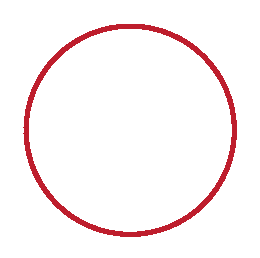
\includegraphics[trim=0cm 0cm 0cm 0cm,clip,scale=0.50]{images/projectivelinesdisk1.pdf}
	\end{minipage}\\
	\begin{minipage}{0.77\textwidth}
	\begin{enumerate}[resume=proj]
			\item Le \textit{rette} con equazione $ax+by=0$, ovvero ai \textit{piani perpendicolari} in $\realset^3$ passanti per le rette con quell'equazione $ax+by=0$:  sul modello piano corrisponde a \textbf{diametri colleganti due punti} sul bordo.
		\end{enumerate}
	\end{minipage}
\begin{minipage}{0.32\textwidth}
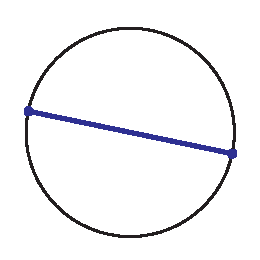
\includegraphics[trim=0cm 0cm 0cm 0cm,clip,scale=0.50]{images/projectivelinesdisk2.pdf}
\end{minipage}\\
\begin{minipage}{0.77\textwidth}
	\begin{enumerate}[resume=proj]
			\item Nel caso generale $ax+by+cz=0$, proiettando l'\textit{arco di cerchio massimo} viene un \textbf{arco di ellisse} in $D$.
		\end{enumerate}
	\end{minipage}
	\begin{minipage}{0.32\textwidth}
		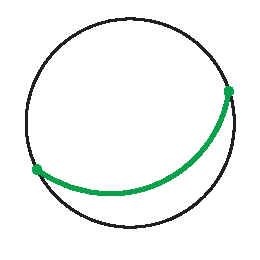
\includegraphics[trim=0cm 0cm 0cm 0cm,clip,scale=0.50]{images/projectivelinesdisk3.pdf}
	\end{minipage}
	\end{itemize}
\vspace{-3mm}
\end{examples}
\section{Operazioni con i sottospazi}
Se $W_1,\ W_2\subseteq V$ sono sottospazi vettoriali, allora $W_1\cap W_2$ è un sottospazio vettoriale e si ha che l'\textbf{intersezione}\index{sottospazio!intersezione} dei corrispettivi spazi proiettivi è ancora un sottospazio proiettivo.
\begin{equation*}
	\proj{W_1\cap W_2}=\proj{W_1}\cap\proj{W_2}
\end{equation*}
\vspace{-6mm}
\begin{observe}
	Si ha:
	\begin{equation*}
		\proj{W_1}\cap\proj{W_2}=\emptyset\iff W_1\cap W_2=\left\{0\right\}
	\end{equation*}
In tal caso diciamo che i due sottospazi sono \textbf{sghembi}\index{sottospazio!proiettivo!sghembo} o \textbf{disgiunti}\seeonlyindex{sottospazio!proiettivo!disgiunto}{sottospazio!proiettivo!sghembo}.
\end{observe}
Come per i sottospazi vettoriali, in generale l'\textbf{unione} di due sottospazi proiettivi \textit{non} è un sottospazio proiettivo.
\begin{define}\textsc{Sottospazio generato da un sottoinsieme}.\\
	Sia $S\subseteq \proj{V}$ un sottoinsieme non vuoto. Il \textbf{sottospazio generato}\index{sottospazio!proiettivo!generato} da $S$, denotato con $\left<S\right>$, è l'intersezione in $\proj{V}$ di tutti i sottospazi proiettivi contenenti $S$, ed è il più piccolo sottospazio contenente $S$.
\end{define}
\begin{itemize}
	\item $\left<S\right>=S\iff S$ è un sottospazio proiettivo.
	\item Se $S=\left\{P_1,\ \ldots,\ P_m\right\}$ è finito, scriviamo $\left<P_1,\ \ldots,\ P_m\right>$ per il sottospazio generato da $P_1,\ \ldots,\ P_m$.
\end{itemize}
\begin{define}\textsc{Sottospazio somma}.\\
	Dati due sottospazi proiettivi $T_1,\ T_2\subseteq \proj{V}$, cioè:
	\begin{equation*}
		T_i=\proj{W_i}\quad W_i\subseteq V,\ i=1,\ 2
	\end{equation*}
	Allora il sottospazio generato da $T_1\cup T_2$ è denotato con $T_1+T_2=\left<T_1,\ T_2\right>$ e si chiama \textbf{sottospazio somma}\index{sottospazio!somma}. In particolare, si ha:
	\begin{equation}
		\left<T_1,\ T_2\right>=\proj{W_1+W_2}
	\end{equation}
\vspace{-6mm}
\end{define}
\begin{demonstration}~{}\\
	$\includedx$ $\proj{W_1+W_2}$ è un sottospazio proiettivo che contiene, in quanto $W_1\subseteq W_1+W_2,\ W_2\subseteq W_1+W_2$ vettorialmente, sia $T_1=\proj{W_1}$ sia $T_2=\proj{W_2}$. In particolare, contiene la loro unione\footnote{Ricordiamo che non è essa un sottospazio, ma un sottoinsieme.}, dunque $\left<T_1,\ T_2\right>\left<T_1\cup T_2\right>\subseteq \proj{W_1+W_2}$.\\
	$\includesx$ Abbiamo che $T_i\subseteq \left<T_1,\ T_2\right>=\proj{U}$, con $U$ un sottospazio vettoriale di $V$. In particolare, si ha che $W_1,\ W_2\subseteq U$, da cui $W_1+W_2\subseteq U$. Passando allo spazio proiettivo:
	\begin{equation*}
		\left<T_1,\ T_2\right>=\proj{U}\subseteq \proj{W_1+W_2}
	\end{equation*}
\vspace{-6mm}
\end{demonstration}
\begin{proposition}\textsc{Formula di Grassmann proiettiva}.\index{formula!di Grassmann proiettiva}\\
	Siano $T_1,\ T_2$ sottospazi proiettivi di $\proj{V}$. Si ha:
	\begin{equation}
				\dim\left<T_1,\ R_2\right>+\dim\left(T_1\cap T_2\right)=\dim T_1+\dim T_2
	\end{equation}
\vspace{-6mm}
\end{proposition}
\begin{demonstration}
	Posti $T_i=\proj{W_i}$, con $W_i\subseteq V$ sottospazi vettoriali. Dalla \textit{formula di Grassmann vettoriale}:
	\begin{equation*}
		\dim\left(W_1+W_2\right)+\dim\left(W_1\cap W_2\right)=\dim W_1+\dim W_2
	\end{equation*}
Sottraendo $1$ a tutte le dimensioni, otteniamo le dimensioni dei corrispettivi spazi proiettivi e dunque la formula proiettiva.
\end{demonstration}
\begin{corollary}
	Siano $T_1,\ T_2$ sottospazi proiettivi di $\proj{V}$ con $\dim\proj{P}=n$. Allora:
	\begin{equation}
		\dim \left(T_1\cap T_2\right)\geq \dim T_1+\dim T_2-n
	\end{equation}
In particolare $T_1\cap T_2\neq \emptyset$ se $\dim T_1+\dim T_2\geq n$.
\end{corollary}
\begin{demonstration}
	\begin{equation*}
		\dim\left(T_1\cap T_2\right)=\dim T_1+\dim T_2-\dim\left<T_1,\ T_2\right>\geq \dim T_1+\dim T_2-n
	\end{equation*}
Chiaramente, se $\dim T_1+\dim T_2\geq n$, allora $\dim \left(T_1\cap T_2\right)\geq 0$ e dunque $T_1\cap T_2\neq \emptyset$.
\end{demonstration}
\begin{example}
	Nel piano proiettivo, due rette sono \textit{sempre incidenti}. Infatti, le rette hanno dimensione $1$, mentre $\dim\proj[2]{\kamp}=2$, dunque vale $1+1\leq 2$, pertanto due rette si incontrano sempre.
\end{example}
\begin{observe}
	Se consideriamo l'insieme \textit{finito di punti}, possiamo considerare lo spazio $S$ \textit{generato} da $P_1,\ \ldots,\ P_m$, cioè $S=\left<P_1,\ \ldots,\ P_m\right>$; inoltre, si ha:
	\begin{equation*}
		\dim S\leq m-1
	\end{equation*}
	Infatti, se $P_i=\left[v_i\right]$ con $v_i\in V$, allora:
	\begin{equation*}
		S=\underbrace{\proj{\lin{v_1,\ \ldots,\ v_m}}}_{\dim \mathcal{L} \leq m}
	\end{equation*}
\vspace{-6mm}
\end{observe}
\section{Punti linearmente indipendenti e in posizione generale}
\begin{define}\textsc{Punti linearmente indipendenti}.\\
	Siano $P_1,\ \ldots, P_m\in\proj{V}$. Diciamo che i punti $P_1,\ \ldots,\ P_m$ sono \textbf{linearmente indipendenti}\index{linearmente indipendenti} se, scelti $v_1,\ \ldots,\ v_m\in V\setminus\left\{0\right\}$ tali che $P_i=\left[v_i\right]\ \forall i$, i vettori $v_1,\ \ldots,\ v_m$ sono \textit{linearmente indipendenti} in $V$.\\
	Se così non è, diciamo che $P_1,\ \ldots, P_m$ sono linearmente dipendenti.
\end{define}
\begin{observes}~{}
	\begin{itemize}
		\item La definizione è \textit{ben posta}. Dati $\lambda_1,\ \ldots,\ \lambda_m\in\kamp\setminus\left\{0\right\}$, si ha che:
		\begin{equation*}
			v_1,\ \ldots,\ v_m\text{ sono indipendenti}\iff\lambda_1 v_1,\ \ldots,\ \lambda_m v_m\text{ sono indipendenti.}
		\end{equation*}
		\item Se $\dim \proj{V}=n$, $\proj{V}$ contiene al più $n+1$ punti indipendenti.
		\item $P_1,\ \ldots,\ P_m$ sono indipendenti se e solo se $\dim\left<P_1,\ \ldots,\ P_m\right>=m-1$.
	\end{itemize}
\end{observes}
\begin{examples}~{}
	\begin{itemize}
		\item \textit{Due} punti $P,\ Q$ sono indipendenti se e solo se $P\neq Q$. Infatti, se $P=\left[v\right]$ e $Q=\left[w\right]$, allora:
		\begin{equation*}
			P\text{ e }Q\text{ sono indipendenti}\iff v\text{ e }w\text{ sono indipendenti}\iff v\nsim w\iff P\neq Q
		\end{equation*}
		In tal caso $\left<P,\ Q\right>$ è l'unico \textit{retta} contenente $P$ e $Q$, che indicheremo anche con $\overline{PQ}$.
		\item \textit{Tre} punti $P_1,\ P_2,\ P_3$ sono indipendenti se e solo se sono \textit{distinti} e \textit{non} sono \textit{allineati}, cioè appartenenti alla stessa retta. In tal caso $\left<P_1,\ P_2,\ P_3\right>$ è l'unico \textit{piano} contenente i tre punti.
	\end{itemize}
\vspace{-3mm}
\end{examples}
\begin{define}\textsc{Punti in posizione generale}.\\
	Dati dei punti $P_1,\ \ldots,\ P_m\in\proj{V}$, diciamo che sono \textbf{in posizione generale}\index{in posizione generale}\index{posizione generale} se vale una delle due condizioni seguenti:
	\begin{itemize}
		\item $m\leq n+1$ e i punti sono \textit{linearmente indipendenti}.
		\item $m>n+1$ e ogni scelta di $n+1$ punti tra loro sono linearmente indipendenti.
	\end{itemize}
\vspace{-3mm}
\end{define}
\begin{example}~{}
		\begin{itemize}
		\item Se $n=1$, cioè $\proj{V}$ è una \textit{retta proiettiva}, allora $P_1,\ \ldots,\ P_m$ sono in posizione generale se e solo se $P_1,\ \ldots,\ P_m$ sono \textit{tutti distinti}.
		\item Se $n=2$, cioè $\proj{V}$ è una \textit{piano proiettivo}, allora $P_1,\ \ldots,\ P_m$ sono in posizione generale se e solo se $P_1,\ \ldots,\ P_m$ sono a $3$ a $3$ \textit{non} allineati.
	\end{itemize}
\vspace{-3mm}
\end{example}
\subsection{Impratichiamoci! Punti linearmente indipendenti}
\begin{exercise}\textsc{F.F.P., 2.1.}\\
	Si mostri che i punti del piano proiettivo reale:
	\begin{equation*}
		\left(\frac{1}{2}\colon 1 \colon 1\right)\quad \left(1\colon \frac{1}{3} \colon \frac{4}{3}\right)\quad \left(2\colon -1 \colon 2\right)
	\end{equation*}
Sono allineati, e si determini un'equazione della retta che li contiene.
\end{exercise}
\begin{solution}
	Per verificare che i $3$ punti sono allineati, dobbiamo verificare che i corrispondenti vettori di $\realset^3$ sono dipendenti. Riscriviamo i seguenti punti per facilitarci i calcoli:
\begin{equation*}
	\left(\frac{1}{2}\colon 1 \colon 1\right)=\left(1\colon 2 \colon 2\right)\quad \left(1\colon \frac{1}{3} \colon \frac{4}{3}\right)=\left(3\colon 1 \colon 4\right)
\end{equation*}
Verifichiamolo la dipendenza con il determinante.
	\begin{equation*}
		\det\left|\begin{array}{ccc}
			1 & 2 & 2\\
			3 & 1 & 4\\
			2 & -1 & 2
		\end{array}\right|=0
	\end{equation*}
L'equazione della retta è data dall'equazione del piano vettoriale in $\realset^3$ generate da $2$ dei $3$ vettori:
\begin{equation*}
	0=\left|\begin{array}{ccc}
		x_0 & x_1 & x_2\\
		1 & 2 & 2\\
		3 & 1 & 4
	\end{array}\right|=x_0\left(8-2\right)-x_1\left(4-6\right)+x_2\left(1-6\right)=6x_0+2x_1-5x_2
\end{equation*}
Verifichiamo che contenga anche il terzo:
\begin{equation*}
	6\cdot 2 + 2\cdot \left(-1\right) -5\cdot 2=0
\end{equation*}
\vspace{-6mm}
\end{solution}
\section{Rappresentazione parametrica di un sottospazio proiettivo}
Sia $S\subseteq\proj{V}$ un sottospazio proiettivo di dimensione $m$. Allora esistono sempre $m+1$ punti $P_0,\ \ldots,\ P_m\in S$ linearmente indipendenti che generano $S$. Infatti, se $S=\proj{W}$ con $W\subseteq V$ sottospazio vettoriale di dimensione $m+1$, possiamo scegliere una base $\left\{w_0,\ \ldots,\ w_m\right\}$ di $W$ tale per cui:
\begin{equation*}
	P_i=\left[w_i\right]\in S
\end{equation*}
Sono linearmente indipendenti (perché lo sono i vettori della base) e generano $S$.\\
Allora, tutti e soli i punti di $S$ sono della forma:
\begin{equation*}
	\left[\lambda_0 w_0+\ldots+\lambda_m w_m\right]\quad \lambda_0,\ \ldots,\ \lambda_m\in\kamp
\end{equation*}
Supponiamo ora di aver fissato una base $\left\{e_0,\ \ldots,\ e_n\right\}$ di $V$ e quindi di aver considerato il corrispondente \textit{riferimento proiettivo}. In coordinate vettoriali di $V$, un punto di $W$ è $x=\left(x_0,\ \ldots,\ x_n\right)$ se e solo se:
\begin{equation*}
	x=x_0e_0+\ldots+x_ne_n=\lambda_0 w_0+\ldots+\lambda_m w_m
\end{equation*}
Il punto $P_i$ in $V$ avrà coordinate $\left(P_{0,i},\ \ldots,\ P_{n,i}\right)\ \forall i=1,\ \ldots,\ m$, dunque il generico vettore $x$ di $W$ è espresso da:
\begin{equation}
	\begin{cases}
		x_0=\lambda_0 P_{0,0}+\lambda_1P_{0,1}+\ldots+\lambda_mP_{0,m}\\
		\vdots\\
		x_n=\lambda_0 P_{n,0}+\lambda_1P_{n,1}+\ldots+\lambda_mP_{n,m}
	\end{cases}
\end{equation}
Anche i punti di $S$ sono date da queste coordinate, dunque questa viene definita la \textbf{rappresentazione parametrica}\index{rappresentazione!parametrica} del sottospazio $S$, con $\left(\lambda_0\colon\ldots\colon\lambda_m\right)$ le coordinate omogenee di $\proj{W}$ date dalla base $\left\{w_0,\ \ldots,\ w_m\right\}$.
\begin{example}
	In $\proj[3]{\realset}$ consideriamo i punti:
	\begin{equation*}
		A=\left(1\colon 0\colon -1\colon 4\right)\quad B=\left(2\colon 3\colon 0\colon 5\right)
	\end{equation*}
Allora, la rappresentazione parametrica del sottospazio $S$ con $\left(\lambda\colon \mu\right)$ è:
\begin{equation*}
	\begin{cases}
		x_0=\lambda+2\mu\\
		x_1=3\mu\\
		x_2=-\lambda\\
		x_3=4\lambda-5\mu
	\end{cases}
\end{equation*}
\vspace{-6mm}
\end{example}
\subsection{Coordinate proiettive e punti in posizione generale}
\begin{observe}
	Sia $\proj{V}$ con un riferimento proiettivo fissato. Consideriamo i punti fondamentali $P_0,\ \ldots,\ P_n$ e il punto unità $U$.
	\begin{itemize}
		\item $P_0,\ \ldots,\ P_n,\ U$ sono $n+2$ punti.
		\item $P_0,\ \ldots,\ P_n,\ U$ sono in posizione generale: essendo $P_i=\left[e_i\right]$ con $e_0,\ \ldots,\ e_n$ base di $V$, allora $P_0,\ \ldots,\ P_n$ sono indipendenti. Se sostituiamo l'$i$-esimo punto con $U=\left[e_1+\ldots+e_n\right]$, allora:
		\begin{equation*}
			P_0,\ \ldots,\ \check{P}_i,\ \ldots,\ U
		\end{equation*}
	Sono indipendenti $\forall i=0,\ \ldots,\ n$.\footnote{Indichiamo con $\check{P}_{i}$ il punto che sostituiamo.}
	\end{itemize}
\vspace{-6mm}
\end{observe}
\begin{observe}
	Sia $\basis=\left\{e_0,\ \ldots,\ e_n\right\}$ una base che induce un \textit{riferimento proiettivo} su $\proj{V}$.\\
	Per ogni $i$ sia $\lambda_i\in\kamp\setminus\left\{0\right\}$ e consideriamo $v_i=\lambda_i e_i$. Allora $\basis'=\left\{v_0,\ \ldots,\ v_n\right\}$ è ancora una base e i \textit{punti fondamentali} del riferimento indotto da $\basis'$ sono \textit{gli stessi} del riferimento indotto da $\basis$. Infatti:
	\begin{equation*}
		\left[e_i\right]=\left[v_i\right]=P_i
	\end{equation*}
	Però i due riferimenti sono \textbf{diversi}; dato $v$ espresso nella base $\basis$:
	\begin{equation*}
		v=x_0e_0+\ldots+x_ne_n
	\end{equation*}
	La sua classe in $\proj{V}$, rispetto a $\basis$, è:
	\begin{equation*}
		\left[v\right]=\left(x_0\colon\ldots\colon x_n\right)
	\end{equation*}
	Possiamo partire dall'espressione di $v$ nella base $\basis$ a quella nella base $\basis'$, moltiplicando e dividendo ogni $e_i$ per il corrispettivo $\lambda_i$:
	\begin{equation*}
		v=\frac{x_0}{\lambda_0}\left(\lambda_0e_0\right)+\ldots+\frac{x_n}{\lambda_n}\left(\lambda_ne_n\right)=\frac{x_0}{\lambda_0}v_0+\ldots+\frac{x_n}{\lambda_n}v_n
	\end{equation*}
	Passiamo dunque alla base $\basis'$ alla classe in $\proj{\kamp}$:
	\begin{equation*}
		\left[v\right]=\left(\frac{x_0}{\lambda_0}\colon\ldots\colon\right)
	\end{equation*}
	Notiamo che effettivamente il punto $\left[v\right]$ non cambia, ma i riferimenti \textit{non} sono multipli e quindi sono diversi!
	\begin{itemize}
		\item \textit{Conoscere} i punti fondamentali \textit{non basta} a determinare la base $\basis$.
		\item Riferimenti proiettivi \textit{diversi} possono avere gli \textit{stessi} punti fondamentali.
	\end{itemize}
\end{observe}
\begin{observe}\label{puntigeneraleindipendentiosserva}
	Supponiamo di avere $n+2$ punti $P_0,\ \ldots,\ P_{n+1}$ in $\proj{V}$, cioè $\forall i=0,\ \ldots,\ n+1\ \exists v_i\in V\ \colon P_i=\left[v_i\right]$. Allora:
	\begin{gather*}
		P_0,\ \ldots,\ P_{n+1}\text{ sono in posizione generale}\iff v_0,\ \ldots,\ v_n\text{ sono indipendenti e}\\
		v_{n+1}=a_0v_0+\ldots+a_nv_n\text{ con }a_i\neq 0\ \forall i=0,\ \ldots,\ n 
	\end{gather*}
Infatti, se $v_0,\ \ldots,\ v_n$ è una base (in quanto sono indipendenti), $v_0,\ \ldots,\ \check{v_i},\ \ldots,\ v_n,\ v_{n+1}$ sono indipendenti se e solo se $a_i\neq 0$.
\end{observe}
\begin{theorema}
	Sia $\proj{V}$ di dimensione $n$. Dati $n+2$ punti $P_0,\ \ldots,\ P_{n+1}$ in \textit{posizione generale}, esiste una base $\basis=\left\{e_0,\ \ldots,\ e_n\right\}$ di $V$ tale che:
	\begin{equation}
		P_0=\left[e_0\right],\ \ldots,\ P_n=\left[e_n\right],\ P_{n+1}=\left[e_0+\ldots+e_n\right]
	\end{equation}
Inoltre, se $\basis'=\left\{f_0,\ \ldots,\ f_n\right\}$ è un'altra base di $V$ che soddisfa la condizione sopra, allora $\basis$ è proporzionale a $\basis$, cioè $\exists\lambda\in\kamp\setminus\left\{0\right\}\ \colon f_i=\lambda e_i\ \forall i=0,\ \ldots,\ n$.
\end{theorema}
\begin{demonstration}
	Sia $P_i=\left[v_i\right]$ al variare di $i=0,\ \ldots,\ n+1$. I punti $P_0,\ \ldots,\ P_n$ sono indipendenti\footnote{Perchè se $N+2$ punti sono in posizione generale, presi $n+1$ punti fra di loro sono indipendenti.}, dunque per definizione $v_0,\ \ldots,\ v_n$ è una base di $V$. Definiamo:
	\begin{equation*}
		v_{n+1}=\lambda_0v_0+\ldots+\lambda_nv_n\quad \lambda_i\in\kamp
	\end{equation*}
	Ma allora, per l'osservazione precedente, $\lambda_i\neq 0\ \forall i$ perché i punti sono in posizione generale.\\
	Consideriamo $_0=\lambda_0v_0,\ e_1=\lambda_1v_1,\ \ldots,\ e_n=\lambda_nv_n$. Si ha che $\basis=\left\{e_0,\ \ldots,\ e_n\right\}$ è una base di $V$ perché $\lambda_i\neq 0$\ $\forall i$. Segue che:
	\begin{gather*}
		\left[e_i\right]=\left[v_i\right]=P_i\ \forall i=0,\ \ldots,\ n\\
		\left[e_0+\ldots+e_n\right]=\left[\lambda_0v_0+\ldots+\lambda_nv_n\right]=\left[v_{n+1}\right]=P_{n+1}
	\end{gather*}
Adesso, sia $\basis')\left\{f_0,\ \ldots,\ f_n\right\}$ come da ipotesi. Allora $\left[f_i\right]=P_i=\left[e_n\right]\ \forall i=0,\ \ldots,\ n$, cioè $\exists \mu_i\in\kamp\setminus\left\{0\right\}\ \colon f_i=\mu_i e_i\ \forall i=0,\ \ldots, n$. Inoltre, soddisfa anche $\left[f_0+\ldots+f_n\right]=P_{n+1}$, pertanto:
\begin{equation*}
	\left[f_0+\ldots+f_n\right]=\left[e_0+\ldots+e_n\right]
\end{equation*}
In altre parole, $\exists \mu\in\kamp\setminus\left\{0\right\}$ tale che:
\begin{equation*}
	\begin{array}{ccc}
		f_0+\ldots+f_n&=&\mu\left(e_0+\ldots+e_n\right)\\
		\shortparallel&&\\
		\mu_0e_0+\ldots+\mu_ne_n&&
	\end{array}
\end{equation*}
$e_0,\ \ldots,\ e_n$ è una base: per l'unicità della scrittura deve essere $\mu=\mu_0=\ldots=\mu_n$, cioè $f_i=\mu e_i\ \forall i=0,\ \ldots,\ n$.
\end{demonstration}
\section{Trasformazioni proiettive}
\begin{define}\textsc{Trasformazione proiettiva e proiettività}.\\
	Un'applicazione $\funz{f}{\proj{V}}{\proj{V'}}$ tra spazi proiettivi si dice \textbf{trasformazione proiettiva}\index{trasformazione proiettiva} o \textbf{isomorfismo proiettivo}\seeonlyindex{isomorfismo!proiettivo}{trasformazione proiettiva} se $\exists \funz{\phi}{V}{V'}$ isomorfismo che induce un altro isomorfismo lineare:
	\begin{equation}
		\begin{tikzcd}
			\widetilde{\phi}\ \colon\\
		\end{tikzcd}
			\funztot{\ }{\proj{V}}{\proj{V'}}{\left[v\right]}{\left[\phi\left(v\right)\right]}
	\end{equation}
	Tale per cui $f=\widetilde{\phi}$.\\
	Se $V=V'$, diciamo che $f$ è una \textbf{proiettività}\index{proiettività} di $\proj{V}$.
\end{define}
\begin{demonstration}~{}
	\begin{itemize}
		\item $\widetilde{\phi}$ \textbf{è ben definita}:
		\begin{enumerate}
			\item $\phi\left(v\right)\neq 0$ perché $v\neq 0$ e $\phi$ è iniettiva, pertanto $\ker\phi=\left\{0\right\}$ e dunque l'unico vettore mappato a $0$ tramite $\phi$ è solo $0$.
			\item Se $\left[v\right]=\left[w\right]$, allora $w\sim v$, cioè $w=\lambda v$ con $\lambda\in\kamp\setminus\left\{0\right\}$; segue che per linearità di $\phi$ $\phi\left(w\right)=\lambda \left(v\right)\implies \left[\phi\left(w\right)\right]=\left[\phi\left(v\right)\right]$
		\end{enumerate}
		\item $\widetilde{\phi}$ \textbf{è iniettiva}: se $\widetilde{\phi}\left(\left[v\right]\right)=\widetilde{\phi}\left(\left[w\right]\right)$, allora
		\begin{equation*}
			\left[\phi\left(v\right)\right]=\left[\phi\left(w\right)\right]\implies\exists\lambda\in\kamp\setminus\left\{0\right\}\ \colon\phi\left(w\right)=\lambda\phi\left(v\right)=\phi\left(\lambda v\right)
		\end{equation*}
	Poichè $\phi$ è iniettiva, segue che $w=\lambda v$ e dunque $\left[v\right]=\left[w\right]$.
		\item $\widetilde{\phi}$ \textbf{è suriettiva}: infatti, se $\left[w\right]\in\proj{V'}$, essendo $\phi$ suriettiva esiste un vettore $v$ tale che $w=\phi\left(v\right)$. Segue che $\left[w\right]=\left[\phi\left(v\right)\right]=\phi\left(\left[v\right]\right)$.
	\end{itemize}
\vspace{-3mm}
\end{demonstration}
Dato che spazi \textit{vettoriali} della \textit{stessa dimensione} sono sempre \textit{isomorfi}, due spazi \textit{proiettivi} della \textit{stessa dimensione} sono sempre \textit{isomorfi} e $\proj{V}$ è sempre isomorfo a $\proj[n]{\kamp}$, con $\dim V=n+1$.
\begin{lemming}
	Siano $\funz{\phi,\ \psi}{V}{V'}$ isomorfismi. Allora:
	\begin{equation}
		\widetilde{\phi}=\widetilde{\psi}\iff\exists\lambda\in\kamp\setminus\left\{0\right\}\ \colon\psi=\lambda\phi
	\end{equation}
\vspace{-6mm}
\end{lemming}
\begin{demonstration}~{}\\
$\impliessx$ Se $v\in\kamp\setminus\left\{0\right\}$, allora $\psi\left(v\right)=\lambda\psi\left(v\right)$. Segue:
\begin{equation*}
	\implies \widetilde{\psi}\left(\left[v\right]\right)=\left[\psi\left(v\right)\right]=\left[\psi\left(v\right)\right]=\widetilde{\psi}\left(\left[v\right]\right)
\end{equation*}
$\impliesdx$ Sia $h\coloneqq \funz{\phi^{-1}\circ \psi}{V}{V}$ automorfismo. Vogliamo mostrare che $h=\lambda Id_V$ con $\lambda\in\kamp\setminus\left\{0\right\}$. Se $v\in V\setminus\left\{0\right\}$, abbiamo:
\begin{equation*}
	\begin{array}{c}
\begin{array}{ccc}
	\widetilde{\phi}\left(\left[v\right]\right)&=&\psi\left(\left[v\right]\right)\\
	\shortparallel&&\shortparallel\\
	\left[\phi\left(v\right)\right]&&\left[\psi\left(v\right)\right]
\end{array}
\implies \lambda_v\in\kamp\setminus\left\{0\right\}\ \colon \phi\left(v\right)=\lambda_v\psi\left(v\right)
\implies h\left(v\right)=\psi^{-1}\left(\phi\left(v\right)\right)=\lambda_v v
\end{array}
\end{equation*}
Segue che $v$ è autovettore di $h\ \forall v\in V\setminus\left\{0\right\}$, in particolare ogni vettore non nullo è autovettore di $h$. Segue che $h$ è diagonalizzabile e ha un unico autovalore $\lambda$. Infatti, presi $\lambda_1$ e $\lambda_2$, si avrebbero i seguenti autovalori indipendenti:
\begin{equation*}
	v_1\in V_{\lambda_1}\setminus\left\{0\right\}\qquad v_2\in V_{\lambda_2}\setminus\left\{0\right\}
\end{equation*}
E considerato che:
\begin{equation*}
	\begin{array}{l}
		h\left(v_1\right)=\lambda_1 v_1\\
		h\left(v_2\right)=\lambda_2 v_2\\
		h\left(v_1+v_2\right)=\lambda\left(v_1+v_2\right)\\
		h\left(v_1+v_2\right)=h\left(v_1\right)+h\left(v_2\right)\\
	\end{array}
	\implies \lambda\left(v_1+v_2\right)=\lambda_1 v_1+\lambda_2 v_2
\end{equation*}
Da cui segue, in quanto $v_1,\ v_2,\ v_1+v_2\neq 0$, che $\lambda=\lambda_1=\lambda_2$ e quindi è unico.\\
Allora, $h=\lambda Id_{V}$ e pertanto $\phi=\lambda \psi$.
\end{demonstration}
\subsection{Gruppo lineare proiettivo}
\begin{observe}
	Consideriamo $\proj{V}$ e l'insieme delle proiettività $\funz{\ }{\proj{V}}{\proj{V}}$.
	\begin{itemize}
		\item La \textit{composizione} di proiettività è una \textit{proiettività} (banalmente \textit{indotta} dalla composizione delle applicazioni lineari).
		\item Poichè $Id_{\proj{V}}=\widetilde{Id_V}\implies$ L'identità $Id_{\proj{V}}$ è una \textit{proiettività}.
		\item Se $\widetilde{\phi}\! \funz{\! }{\proj{V}}{\proj{V}}$, allora $\widetilde{\phi^{-1}}=\funz{f^{-1}}{\proj{V}}{\proj{V}}$. In altre parole, l'\textit{inversa} di una proiettività è ancora una proiettività.
	\end{itemize}
L'insieme delle proiettività risulta un \textbf{gruppo} rispetto alla \textit{composizione}.
\end{observe}
\begin{define}\textsc{Gruppo lineare proiettivo}.\\
Il \textbf{gruppo lineare proiettivo}\index{gruppo!lineare proiettivo} $\projgl{V}$ è il gruppo delle proiettività dello spazio vettoriale $V$ con operazione la composizione di proiettività ed elemento neutro $Id_{\proj{V}}$.
\vspace{-3mm}
\end{define}
\subsubsection{Descrizione matriciale del gruppo lineare proiettivo}
Consideriamo gli isomorfismi $\funz{\ }{\kamp^{n+1}}{\kamp^{n+1}}$: sappiamo che la matrice associata agli isomorfismi è una matrice invertibile, cioè si ha una \textit{isomorfismo di gruppi} fra l'insieme degli isomorfismi in $\kamp^{n+1}$ al \textit{gruppo generale lineare} $\gl\left(n+1,\ \kamp\right)$:
\begin{equation*}
	\left\{\text{isomorfismi}\funz{\ }{\kamp^{n+1}}{\kamp^{n+1}}\right\}\leftrightarrow\gl\left(n+1,\ \kamp\right)
\end{equation*}
E con il gruppo lineare proiettivo si può fare? Consideriamo:
\begin{equation}
	\funztot{\oldphi}{\gl\left(n+1,\ \kamp\right)}{\projgl[n+1]{\kamp}}{\phi_A}{\widetilde{\phi}_A}
\end{equation}
 $\phi$ è \textit{omomorfismo} di gruppi \textit{suriettivo}, ma non iniettivo. Infatti, il nucleo non è \textit{triviale}:
 \begin{equation*}
 	\ker \oldphi=\left\{\phi_A\mid \phi_A=Id_{\proj[n]{\kamp}}=\widetilde{Id}_{\kamp^{n+1}}\right\}=\left\{\phi_A\mid \phi=\lambda I,\ \lambda\in\kamp\setminus\left\{0\right\}\right\}=\left\{\phi_A\mid A=\lambda I,\ \lambda\in\kamp\setminus\left\{0\right\}\right\}
 \end{equation*}
Tuttavia, possiamo per il Teorema dell'isomorfismo per i gruppi considerare il seguente diagramma commutativo:
\[\begin{tikzcd}
	{\gl\left(n+1,\ \kamp\right)} & {\projgl[n+1]{\kamp}} \\
	{\frac{\gl\left(n+1,\ \kamp\right)}{\left\{\lambda I\ \mid\ \lambda\in\kamp\setminus\left\{0\right\}\right\}}}
	\arrow["{\pi}"', from=1-1, to=2-1]
	\arrow["{\exists \overline f}"', from=2-1, to=1-2, dashed]
	\arrow["{\oldphi}", from=1-1, to=1-2]
\end{tikzcd}\]
E si ha pertanto l'isomorfismo:
\begin{equation*}
	\projgl[n+1]{\kamp}\cong \frac{\gl\left(n+1,\ \kamp\right)}{\left\{\lambda I\mid\lambda\in\kamp\setminus\left\{0\right\}\right\}}=\frac{\gl\left(n+1,\ \kamp\right)}{\left\{\lambda I\right\}}
\end{equation*}
Si può anche considerare l'isomorfismo tra $\left\{\lambda I\mid\lambda\in\kamp\setminus\left\{0\right\}\right\}$ e $\kamp\setminus\left\{0\right\}$, e riscrivere l'isomorfismo trovato come:
\begin{equation*}
	\projgl[n+1]{\kamp}\cong \frac{\gl\left(n+1,\ \kamp\right)}{\kamp\setminus\left\{0\right\}}
\end{equation*}

\begin{example}
	Consideriamo la seguente proiettività della \textit{retta proiettiva} $\proj[1]{\realset}$:
	\begin{equation*}
		\funztot{f}{\proj[1]{\realset}}{\proj[1]{\realset}}{\left(x_0\colon x_1\right)}{\left(ax_0+bx_1\colon cx_0+dx_1\right)}
	\end{equation*}
	Considerato il gruppo lineare proiettivo $\proj[2]{\realset}=\frac{\gl\left(2,\ \realset\right)}{\left\{\lambda I\right\}}$, per definizione di $f$ si ha $f=\widetilde{\phi}$. In particolare, la matrice associata a $\phi$ è:
	\begin{equation*}
		A=\left(\begin{array}{cc}
			a & b\\
			c & d
		\end{array}\right)
	\end{equation*}
	E dunque possiamo scrivere l'applicazione lineare $\phi$ come:
	\begin{equation*}
		\funztot{f}{\realset^2}{\realset^2}{\left(\begin{array}{c}
				x_0 \\
				x_1
			\end{array}\right)}{A\left(\begin{array}{c}
				x_0 \\
				x_1
			\end{array}\right)}
	\end{equation*}
	E dunque $f$ si può anche scrivere come:
	\begin{equation*}
		\funztot{f}{\proj[1]{\realset}}{\proj[1]{\realset}}{\left[v\right]}{\left[Av\right]}
	\end{equation*}
	Notiamo che se la matrice associata a $\phi$ fosse $2A$, per \textit{proporzionalità} si avrebbe comunque la proiettività $f$. In modo analogo, $\lambda\in\realset\setminus\left\{0\right\}$ induce la \textit{stessa proiettività} $f$ di $A$.
	\vspace{-3mm}
\end{example}
\subsection{Altri aspetti delle trasformazioni proiettive}
\begin{observe}
	Se $f$ è una proiettività di $\proj{V}$ e $S\subseteq \proj{V}$ un sottospazio proiettivo, allora $f\left(S\right)$ è ancora un sottospazio proiettivo della stessa dimensione di $S$. Se $S=\proj{W}$ e consideriamo per definizione $f=\widetilde{\phi}$ con $\funz{\phi}{V}{V}$, allora:
	\begin{equation*}
		\forall \left[v\right]\in S\ f\left(\left[v\right]\right)=\widetilde{\phi}\left(\left[v\right]\right)=\left[\phi\left(v\right)\right],\ \phi\left(v\right)\in W
	\end{equation*}
	\begin{equation}
		f\left(S\right)=\proj{\phi\left(W\right)}
	\end{equation}
\vspace{-6mm}
\end{observe}
\begin{define}\textsc{Proiettivamente equivalenti}.\\
	Due sottoinsiemi $A,\ B$ di $\proj{V}$ si dicono \textbf{proiettivamente equivalenti}\index{proiettivamente equivalenti} se $\exists f$ proiettività di $\proj{V}$ tale che:
	\begin{equation}
		B=f\left(A\right)
	\end{equation}
\vspace{-6mm}
\end{define}
\begin{example}
	Due sottospazi proiettivi di $\proj{V}$ della \textit{stessa} dimensione sono sempre \textit{proiettivamente equivalenti}.
\end{example}
\begin{theorema}\label{puntigeneralitrasformazioni}
	Siano $\proj{V}$ e $\proj{V'}$ di dimensione $n$. Siano:
	\begin{itemize}
		\item $P_0,\ \ldots,\ P_{n+1}\in\proj{V}$ $n+2$ punti in posizione generale.
		\item $Q_0,\ \ldots,\ Q_{n+1}\in\proj{V'}$ $n+2$ punti in posizione generale.
	\end{itemize}
Allora $\exists!\funz{f}{\proj{V}}{\proj{V'}}$ trasformazione proiettiva tale che $f\left(P_i\right)=Q_i\ \forall i=0,\ \ldots,\ n+1$.\\
In particolare: se una proiettività fissa $n+2$ punti ($f\left(P_i\right)=P_i\ \forall i=0,\ \ldots,\ n+1$) in posizione generale, allora è l'identità.
\end{theorema}
\begin{demonstration}~{}
	\begin{itemize}
		\item \textbf{Esistenza}: Siano, $\forall i$:
		\begin{itemize}
			\item $P_i=\left[v_i\right]\ v_i\in V$.
			\item $Q_i=\left[w_i\right]\ w_i\in V'$.
		\end{itemize}
	Sappiamo, dall'osservazione a pag. \ref{puntigeneraleindipendentiosserva}, che:
	\begin{itemize}
		\item $v_0,\ \ldots,\ v_n$ è base di $V$, con $v_{n+1}=\lambda_0v_0+\ldots+\lambda_n v_n$ con $\lambda_i\neq 0\ \forall i$.
		\item $w_0,\ \ldots,\ w_n$ è base di $V'$, con $w_{n+1}=\mu_0w_0+\ldots+\mu_n w_n$ con $\mu_i\neq 0\ \forall i$.
	\end{itemize}
		A meno di cambiare i rappresentanti dei punti, possiamo supporre senza perdita di generalità che $\lambda_i=\mu_i=1$. Si ha dunque:
		\begin{gather*}
			v_{n+1}=v_0+\ldots+v_n\\
			w_{n+1}=w_0+\ldots+w_n
		\end{gather*}
	Sia $\funz{\phi}{V}{V'}$ l'applicazione lineare tale per cui $\phi\left(v_i\right)=w_i\ \forall i=0,\ \ldots,\ n$. Per linearità:
	\begin{equation*}
		\phi\left(v_{n+1}\right)=\phi\left(v_0+\ldots+v_n\right)=\phi\left(v_0\right)+\ldots+\phi\left(v_n\right)=w_0+\ldots+w_n=w_{n+1}
	\end{equation*}
Poiché $\im \phi$ contiene una base per costruzione, $\phi$ è suriettiva. In particolare, essendo endomorfismo ($\dim V=\dim V'$), $\phi$ è anche \textit{isomorfismo}.\\
Allora $f\coloneqq\widetilde{\phi}\funz{\ }{\proj{V}}{\proj{V'}}$ è una \textit{trasformazione proiettiva} e:
\begin{equation*}
	f\left(P_i\right)=f\left(\left[v_i\right]\right)=\left[\phi\left(v_i\right)\right]=\left(w_i\right)=Q_i\ \forall i=0,\ \ldots,\ n+1
\end{equation*}
\item \textbf{Unicità}: sia $\funz{g}{\proj{V}}{\proj{V'}}$ un'altra trasformazione proiettiva tale che $g\left(P_i\right)=Q_i\ \forall i=0,\ \ldots,\ n+1$. Per definizione, esiste $\funz{\psi}{V}{V'}$ isomorfismo per cui $g=\widetilde{\psi}$ e:
\begin{equation*}
	\left[\psi\left(v_i\right)\right]=\left[w_i\right]\ \forall i
\end{equation*}
Si ha che $\exists a_i\in\kamp\setminus\left\{0\right\}$ tale che $\psi\left(v_i\right)=a_iw_i$. Allora:
\begin{equation*}
	\begin{array}{ccccc}
		a_{n+1}w_{n+1}&=&\psi\left(v_{n+1}\right)&=&\psi\left(v_0+\ldots+v_n\right)\\
		\shortparallel&&&&\shortparallel\\
		a_{n+1}\left(w_0+\ldots+w_n\right)&&&&\psi\left(v_0\right)+\ldots+\psi\left(v_n\right)\\
		\shortparallel&&&&\shortparallel\\
		a_{n+1}w_0+\ldots+a_{n+1}w_n&&&&a_0w_0+\ldots+a_nw_n
	\end{array}
\end{equation*}
Poiché $w_0,\ \ldots,\ w_n$ è base, la scrittura è unica. Segue che $a_0=a_1=\ldots=a_{n+1}=a$. Allora:
\begin{equation*}
	\begin{array}{l}
		\psi\left(v_i\right)=aw_i=a\phi\left(v_i\right)\\
		\implies \psi=a\phi\\
		\implies g=\widetilde{\psi}=\widetilde{\phi}=f
	\end{array}
\end{equation*}
	\end{itemize}
\vspace{-6mm}
\end{demonstration}
\begin{examples}
	\begin{itemize}
		\item In una \textit{retta proiettiva} ($\dim 1$), una proiettività è determinata dalle immagini di $3$ \textit{punti distinti}, dato che è equivalente alla condizione di ‘‘\textit{punti in posizione generale}''.
		\item In un \textit{piano proiettivo} ($\dim 2$), una proiettività è determinata dalle \textit{immagini} di $4$ punti, a $3$ a $3$ \textit{non allineati}.
		\item Se $A,\ B\subseteq \proj{V}$ sono insiemi finiti, ciascuno contenente $k$ punti in posizione generale, con $k\leq n+2$, allora $A$ e $B$ sono sempre proiettivamente equivalenti.
	\end{itemize}
\vspace{-3mm}
\end{examples}
\begin{example}
	Approfondiamo l'ultimo esempio. In $\proj[2]{\kamp}$ ($\dim 2$), si prenda $A=\left\{P_1,\ P_2\right\},\ B=\left\{Q_1,\ Q_2\right\}$ con $P_1\neq P_2$, $Q_1\neq Q_2$. Ho due punti distinti sia in $A$ e $B$, dunque esiste sempre una proiettività $\funz{f}{\proj[2]{\ }}{\proj[2]{\ }}$ tale che $f\left(A\right)=B$.\\
	Se invece $A$ e $B$ contengono $3$ punti, se i $3$ punti in $A$ \textit{sono allineati} mentre i $3$ punti in $B$ \textit{non} lo sono, allora $A$ e $B$ \textit{non} sono proiettivamente equivalenti.
\end{example}
\subsection{Trasformazioni proiettive in coordinate}
Supponiamo di avere fissato dei \textit{riferimenti proiettivi} su $\proj{V}$ e $\proj{V'}$, dati da delle basi $\basis$ di $V$ e $\basis'$ di $V'$, e sia $\funz{f}{\proj{V}}{\proj{V}}$ una trasformazione proiettiva. Sappiamo che $f=\widetilde{\phi}$ con $\funz{\phi}{V}{V'}$ isomorfismo lineare.\\
Sia $A\in\gl\left(n+1,\ \kamp\right)$ la matrice associata a $\phi$ rispetto alle basi $\basis$ e $\basis'$. Abbiamo visto che $\phi$ è determinata solo a meno di multipli: chiaramente, lo stesso è vero anche per $A$.\\
Siano allora:
\begin{gather*}
	P=\left(x_0\colon\ldots\colon x_n\right)\in\proj{V}\\
	f\left(P\right)=\left(y_0\colon\ldots\colon y_n\right)\in\proj{V'}
\end{gather*}
Allora $\exists\rho\in\kamp\setminus\left\{0\right\}$ tale che $\rho y=Ax$.
\begin{observe}\textsc{Cambiamenti di coordinate.}\\
Se in $\proj{V}$ abbiamo due riferimenti proiettivi, uno dalla dalla base $\basis$, e uno dalla base $\basis'$, sia $M$ la \textit{matrice del cambiamento di base} in $V$ tale che:
\begin{equation*}
	x'=Mx
\end{equation*}
Con $x$ in coordinate rispetto alla base $\basis$ e $x'$ in coordinate rispetto alla base $\basis'$. Allora, se $P\in\proj{V}$ ha coordinate:
\begin{equation*}
	\left(x_0\colon\ldots\colon x_n\right)\text{ rispetto a }\basis\\
	\left(x_0'\colon\ldots\colon x_n'\right)\text{ rispetto a }\basis'
\end{equation*}
Esiste $\rho\in\kamp\setminus\left\{0\right\}$ tale che $\rho x'=M x$.
\end{observe}
\subsection{Punti fissi di proiettività}
\begin{define}\textsc{Punto fisso}.\\
	Sia $\funz{f}{\proj{V}}{\proj{V}}$ una proiettività. Un \textbf{punto fisso}\index{punto!fisso} è un punto $P\in\proj{V}$ tale che:
	\begin{equation}
		f\left(P\right)=P
	\end{equation}
\vspace{-6mm}
\end{define}
Sia $\funz{\phi}{V}{V}$ un \textit{automorfismo} tale che $f=\widetilde{\phi}$, e sia $P=\left[v\right]$, con $v\in V\setminus\left\{0\right\}$. Allora:
\begin{equation*}
	\begin{array}{ll}
		& f\left(P\right)=\left[\phi\left(v\right)\right]=\left[v\right]\\
		\iff & \exists\lambda\in\kamp\setminus\left\{0\right\}\ \colon \phi\left(v\right)=\lambda v\\
		\iff & v\text{ è un autovettore per }\phi
	\end{array}
\end{equation*}
In particolare, $\phi$ è invertibile, dunque \textit{non} ha l'autovettore \textit{nullo}. Segue che i punti fissi di $f$ sono tutti e soli i punti $\left[v\right]$ con $v$ autovettore di $\phi$.
\begin{observes}~{}
	\begin{enumerate}
		\item Se $\kamp=\complexset$, allora ogni proiettività ha almeno un punto fisso, dato che $\phi$ ha sempre almeno un autovettore.
		\item Se $\kamp=\realset$ e $\dim\proj{V}=n$, allora $\dim V=n+1$. Il \textit{polinomio caratteristico} $C_\phi\left(t\right)\in\realset\left[t\right]$ ha grado $n+1$. Se $n$ è \textit{pari}, $\phi$ ha almeno un autovalore, dato che il polinomio caratteristico ha grado $n+1$ \textit{dispari}: infatti, o è di grado \textit{uno} (e quindi ha banalmente soluzione) oppure, in quanto si può decomporre in fattori a coefficienti reali al più di grado \textit{due}, ammetterà \textit{sempre} almeno un fattore di grado \textit{uno}.
		\item Portiamo un controesempio al caso $n$ dispari. Sia $\funztot{f}{\proj{\realset}}{\proj{\realset}}{\left(x\colon y\right)}{\left(-y\colon x\right)}$. La matrice $A$ associata a $f$ è:
		\begin{equation*}
			A=\left(\begin{array}{cc}
				0 & -1 \\ 
				1 & 0
			\end{array}\right)
		\end{equation*}
	Il polinomio caratteristico \textit{non} ha radici \textit{reali}:
	\begin{equation*}
		C_A\left(t\right)=\det\left(\begin{array}{cc}
			-t & -1 \\ 
			1 & -t
		\end{array}\right)=t^2-1
	\end{equation*}
Segue che $A$ non ha autovettori reali e pertanto $f$ \textit{non} ha punti fissi.
\item In generale, l'\textit{insieme} dei punti fissi di $\funz{f}{\proj{V}}{\proj{V}}$ è dato da:
\begin{equation*}
	\left\{\proj{V_{\lambda}}\mid\lambda\text{ autovalore di }\phi\right\}
\end{equation*}
Questo è un insieme di sottospazi proiettivi a 2 a 2 disgiunti.
 	\end{enumerate}
\end{observes}
\begin{define}\textsc{Insieme fisso.}\\
	Se $S\subseteq\proj{V}$ è un sottospazio, diciamo che $S$ è \textbf{fisso} per $f$ proiettività se:
		\begin{equation}
		f\left(S\right)=S
	\end{equation}
	\vspace{-6mm}
\end{define}
\subsection{Impratichiamoci! Trasformazioni proiettive}
\begin{exercise}
	In $\proj[1]{\realset}$ determinare la proiettività $f$ tale che:
	\begin{equation*}
		f\left(2\colon 1\right)=\left(1\colon1\right)\quad f\left(1\colon 2\right)=\left(0\colon1\right)\quad
		f\left(1\colon -1\right)=\left(1\colon0\right)
	\end{equation*}
\vspace{-6mm}
\end{exercise}
\begin{solution}
Notiamo che i punti:
\begin{equation*}
	\left(2\colon 1\right)\quad\left(1\colon 2\right)\quad\left(1\colon -1\right)\text{ e }	\left(1\colon 1\right)\quad\left(0\colon 1\right)\quad\left(1\colon 0\right)
\end{equation*}
Sono distinti, dunque sono in posizione generale e la proiettività è garantita. Prendiamo la generica matrice $A=\left(\begin{array}{cc}
	a & b\\
	c & d
\end{array}\right)$ associata a $\phi$ indotta da $f$ e consideriamo $\rho y=Ax$:
\begin{equation*}
	\begin{cases}
		\rho y_0=ax_0+bx_1\\
		\rho y_1=cx_0+dx_1
	\end{cases}
\end{equation*}
Imponiamo il passaggio per $f\left(2\colon 1\right)=\left(1\colon1\right)$:
\begin{equation*}
	\begin{cases}
		\rho=1a+b\\
		\rho=2c+d
	\end{cases}\implies 2a+b=2c+d
\end{equation*}
In sostanza, \textit{eliminiamo} il parametro $\rho$ per ottenere un'equazione lineare \textit{omogenea} tra gli elementi della matrice.\\
Facciamo lo stesso con i rimanenti punti $f\left(1\colon 2\right)=\left(0\colon1\right)$ e $	f\left(1\colon -1\right)=\left(1\colon0\right)$, utilizzando rispettivamente $\mu y=Ax$ e $\alpha y=Ax$:
\begin{gather*}
	\begin{cases}
		0=a+2b\\
		\rho=c+2d
	\end{cases}\implies a+2b=0\\
	\begin{cases}
		\alpha=a-b\\
		0=c-d
	\end{cases}\implies c-d=0
\end{gather*}
Costruiamo così un sistema lineare omogeneo di $3$ equazioni in $4$ incognite $a,\ b,\ c,\ d$, con una matrice dei coefficienti di rango $3$:
\begin{equation*}
	\begin{cases}
		2a+b=2c+d\\
		a+2b=0\\
		c-d=0
	\end{cases}\implies \begin{cases}
	a=2c\\
	b=-c\\
	c=c\\
	d=c
\end{cases}\implies
A=\left(\begin{array}{cc}
	2c & -c\\
	c & c
\end{array}\right)=c\left(\begin{array}{cc}
1 & -1\\
1 & 1
\end{array}\right)
\end{equation*}
A meno di multipli, $A=\left(\begin{array}{cc}
	1 & -1\\
	1 & 1
\end{array}\right)$ è la matrice cercata. Segue dunque che la proiettività cercata è:
\begin{equation*}
	\funztot{f}{\proj[1]{\realset}}{\proj[1]{\realset}}{\left(x_0\colon x_1\right)}{\left(2x_0-x_1\colon x_0+x_1\right)}
\end{equation*}
\vspace{-3mm}
\end{solution}
\section{Geometria affine e geometria proiettiva}\label{spaziaffini}
Abbiamo già accennato all'esistenza di una relazione che intercorre fra \textit{geometria affine} e \textit{geometria proiettiva}. Diamo innanzitutto qualche richiamo dei concetti della geometria affine.
\begin{define}\textsc{Spazio affine}.\\
	Sia $V$ uno spazio vettoriale di dimensione finita su un campo $\kamp$. Uno \textbf{spazio affine}\index{spazio!affine} di dimensione $n$ su $V$ (con spazio vettoriale associato $V$ di dimensione $n$ ) è un insieme $\aff{V}$ non vuoto di \textit{punti} (elementi) tale che sia data un'applicazione:
	\begin{equation*}
		\funztot{\ }{\aff{V}\times\aff{V} }{V}{\left(P,\ Q\right)}{\overrightarrow{PQ}}
	\end{equation*}
	Che alla coppia di punti $\left(P,\ Q\right)$ associa il vettore di $V$ con punto iniziale $P$ e punto finale $Q$ e tale che siano
	soddisfatti i seguenti assiomi:
	\begin{enumerate}
		\item $\forall P\in\aff{V},\ \forall v\in V$ esiste un unico punto $Q\in\aff{V}$ tale che $\overrightarrow{PQ}=v$.
		\item $\forall P,\ Q,\ R\in\aff{V}$ terna di punti di $\aff{V}$ si ha $\overrightarrow{PQ}+\overrightarrow{QR}=\overrightarrow{PR}$.
	\end{enumerate}
\end{define}
\begin{define}\textsc{Riferimento affine e coordinate affini}.\\
	Un \textbf{riferimento affine}\index{riferimento!affine} $\mathcal{R} = (O,\  e_1,\  e_2,\ \ldots,\  e_n)$ sullo spazio $\aff{V}$ è assegnato fissando un punto $O\in \aff{V}$ detta \textbf{origine}\index{origine!affine} ed una base $\basis = (e_1,\  e_2,\ \ldots,\  e_n)$ di $V$. Dunque, per ogni $P\in \aff{V}$ si ha la $n$-upla $(X_1,\  X_2,\ \ldots,\  X_n)$ dette \textit{coordinate affini}\index{coordinate!affini} del punto $P\in\aff{V}$ (uniche per riferimento affine fissato) tale per cui:
	\begin{equation}
		P=\overrightarrow{OV}=x_1e_1+\ldots+x_ne_n
	\end{equation}
\vspace{-6mm}			 
\end{define}
Per i nostri scopi, parleremo spesso degli spazi affini di dimensione $n$ su $\kamp$.
\begin{define}\textsc{Affinità}.\\
	Un'\textbf{affinità}\index{affinità} o \textbf{trasformazione lineare affine}\seeonlyindex{trasformazione lineare affine}{affinità} di $\aff{\kamp^n}$ è un'applicazione:
	\begin{equation}
		\funz{\phi}{\aff{\kamp^n}}{\aff{\kamp^n}}
	\end{equation}
Della forma $\phi\left(x\right)=Ax+b$ con $A\in\gl\left(n,\ \kamp\right)$ un'applicazione lineare invertibile e $b$ una \textit{traslazione}.
\end{define}
\begin{define}\textsc{Sottospazio affine}.\\
	Un \textbf{sottospazio affine}\index{sottospazio!affine} di $\aff{\kamp^n}$ è un \textit{traslato} di un sottospazio vettoriale $W\subseteq \kamp^n$:
	\begin{equation}
		S=W+x_0=\left\{w+x_0\mid w\in W,\ x_0\in\aff{W}\right\}
	\end{equation}
\vspace{-6mm}
\end{define}
\begin{observes}~{}
	\begin{itemize}
		\item $W$ è l'unico traslato di $S$ per l'origine ($x_0=O$) e si dice \textbf{sottospazio direttore}  di $S$\index{sottospazio!direttore}, cioè ne dà appunto la \textit{direzione}. Si definisce $\dim S\coloneqq\dim W$.
		\item Un punto in $\aff{\kamp^n}$ è un sottospazio affine di dimensione $0$ ($W=\left\{0\right\}$; dopotutto non ha particolarmente senso parlare di direzione del punto).
		\item Una \textbf{retta affine}\index{retta!affine} $r$ in $\aff{\kamp^n}$ è un sottospazio affine di $\dim 1$: $W=\lin{v}$, cioè $r$ si può individuare assegnando un punto $P\in r$ e un qualsiasi vettore $v$ \textit{parallelo} alla retta $r$.
		\item Un \textbf{piano affine}\index{piano!affine} $\pi$ in $\aff{\kamp^n}$ è un sottospazio affine di $\dim 2$: $W=\lin{v,\ w}$, cioè $\pi$ si può individuare assegnando un punto $P\in r$ e una coppia di vettori l.i. \textit{paralleli} al piano $\pi$.
		\item Un \textbf{iperpiano affine}\index{iperpiano!affine} è un sottospazio di dimensione $n+1$.
		\item Due sottospazi affini della stessa dimensione si dicono \textbf{paralleli}\index{parallelo} se hanno lo \textit{stesso} sottospazio direttore.
	\end{itemize}
\vspace{-3mm}			 
\end{observes}
\begin{example}
Consideriamo $r=W+x_0$ retta affine, che ha dunque $\dim r=\dim W=1$. $W$ è la retta vettoriale in $\kamp^n$, mentre un qualunque $v\in W\setminus\left\{0\right\}$ è la \textit{direzione} della retta.
\end{example}
Un sottospazio affine $S\subseteq \kamp^n$ può essere descritti con equazioni cartesiane oppure in forma parametrica.\\
	\textbf{Equazioni cartesiane}. $S$ è visto come l'insieme delle \textit{soluzioni} del seguente sistema lineare:
	\begin{equation}
		Ax=b\qquad\left(\begin{array}{c}
			X_1\\
			\vdots\\
			X_n
		\end{array}\right)\in\aff{\kamp^{n}}
	\end{equation}
Con $b$ che descrive la traslazione dovuta a $x_0\in\aff{W}$.
In tal caso $W$ è il sottospazio vettoriale delle soluzioni del sistema lineare omogeneo associato:
\begin{equation}
	Ax=0
\end{equation}
\textbf{Forma parametrica}. Supponiamo $\dim S=\dim W=m$. Siano $v_1,\ \ldots,\ v_m\in\kamp^n$ i vettori di una base di $W$; rispetto ad una base di $\kamp^n$, e dunque rispetto ad un sistema di riferimento affine con origine $O$, essi sono espressi nelle componenti:
\begin{equation*}
	v_i=\left(V_{i,1},\ \ldots,\ V_{i,n}\right)\in\aff{\kamp^n}
\end{equation*}
Consideriamo $S=W+c$, con il punto $c=\left(C_1,\ \ldots,\ C_n\right)$ rispetto allo stesso sistema affine di prima.\\
I punti $x$ di $S$ in forma parametrica sono dati da:
\begin{equation}
	x=t_1v_1+\ldots+t_mv_m+c\quad t_1,\ \ldots,\ t_m\in\kamp
\end{equation}
Da cui otteniamo il sistema $n\times\left(m+1\right)$ seguente:
\begin{equation}
	\begin{cases}
		\begin{array}{l}
			X_1=t_1V_{1,1}+\ldots+t_mV_{m,1}+C_1\\
			\vdots\\
			X_n=t_1V_{1,n}+\ldots+t_mV_{m,n}+C_n\\			
		\end{array}
	\end{cases}
\end{equation}
\begin{example}
	La retta $r$ ($\dim W=1$) passante per $c$ con direzione $v$ è descritto parametricamente da:
\begin{equation*}
	\begin{cases}
		\begin{array}{l}
			X_1=tV_1+c_1\\
			\vdots\\
			X_n=tV_n+c_n			
		\end{array}
	\end{cases}
\end{equation*}	
\end{example}
Consideriamo ora lo \textit{spazio proiettivo numerico}:
\begin{equation*}
	\proj[n]{\ }=\proj[n]{\kamp}=\proj{\kamp^{n+1}}
\end{equation*}
E i punti in coordinate omogenee $\left(x_0\colon \ldots\colon x_n\right)$ rispetto ad un dato sistema di riferimento proiettivo.
Consideriamo il seguente sottoinsieme di $\proj[n]{\ }$:
\begin{equation}
	U_0\coloneqq \left\{P=\left(x_0\colon\ldots\colon x_n\right)\in \proj[n]{\ }\mid x_0\neq 0\right\}
\end{equation}
La condizione $x_0\neq 0$ è \textit{ben posta}; infatti, se $\lambda\in\kamp\setminus\left\{0\right\}$, allora $x_0\neq 0\iff\lambda x_0\neq 0$.\\
Consideriamo anche il suo complementare, che è l'iperpiano coordinato rispetto alla prima coordinata omogenea:
\begin{equation}
	\proj[n]{\ }\setminus=H_0=\left\{P=\left(x_0\colon\ldots\colon x_n\right)\in \proj[n]{\ }\mid x_0= 0\right\}=\left\{P=\left(0\colon\ldots\colon x_n\right)\in \proj[n]{\ }\right\}
\end{equation}
Sia $P\in U_0$: allora essendo $a_0\neq 0$ si ha $P=\left(a_0\colon\ldots\colon a_n\right)=\left(1\colon\frac{a_1}{a_0}\ldots\colon \frac{a_n}{a_0}\right)$. In particolare, $\frac{a_1}{a_0},\ \ldots,\ \frac{a_n}{a_0}$ sono univocamente determinate da $P$.
\begin{example}
 Sia $\proj[2]{\realset}=\left\{\text{rette vettoriali in }\realset^3\right\}$ con punti di componenti $\left(x_0\colon x_1\colon x_2\right)$. Allora $H_0$ è una retta proiettiva in $\proj[2]{\realset}$ e risulta:
 \begin{equation*}
 	\begin{array}{ll}
 		H_0 & =\left\{P=\left(x_0\colon x_1\colon x_2\right)\in \proj[n]{\ }\mid x_0=0\right\}=\left\{P=\left(0\colon x_1\colon x_2\right)\in \proj[n]{\ }\right\} \\
 		& =\left\{\text{rette vettoriali di }\realset^3\text{ contenute nel piano affine }x_0=0\right\}
 	\end{array}
 \end{equation*}
	Infatti, prendiamo $\aff{\realset^3}$ e consideriamo il piano $x_0=1$, parallelo al piano $x_0=0$. Se $r\subseteq \realset^3$ è una retta vettoriale che \textit{non} appartiene al piano affine $\left\{x_0=0\right\}$ ($r\nsubseteq \left\{x_0=0\right\}$), $r$ interseca il piano $x_0=1$ in un solo punto! In particolare, se $r$ ha direzione $\left(a_0,\ a_1,\ a_2\right)$, il punto nel piano $\left\{x_0=1\right\}$ avrà coordinate $\left(\frac{a_1}{a_0},\ \frac{a_2}{a_0}\right)$.
\end{example}
Possiamo identificare $U_0\subseteq\proj[n]{\ }$ con $\aff{\kamp^n}$. Consideriamo le due funzioni seguenti:
\begin{equation}
	\funztot{j=j_0}{\aff{\kamp^n}}{U_0\subseteq \proj[n]{\ }}{\left(X_1,\ \ldots,\ X_n\right)}{\left(1\colon\ x_1\colon \ldots\colon X_n\right)}\\
	\funztot{\oldphi}{U_0\subseteq \proj[n]{\ }}{\aff{\kamp^n}}{\left(x_0\colon\ \ldots\colon X_n\right)}{\left(\frac{x_1}{x_0},\ \ldots,\ \frac{x_n}{x_0}\right)}
\end{equation}
\begin{itemize}
	\item $\oldphi$ è ben definita, dato che $x_0\neq 0$ per definizione di $U_0$.
	\item $j$ e $\oldphi$ sono l'una l'inversa dell'altra:
	% https://q.uiver.app/?q=WzAsNixbMCwwLCJcXGFmZntcXGthbXBebn0iXSxbMSwwLCJVXzAiXSxbMiwwLCJcXGFmZntcXGthbXBebn0iXSxbMCwxLCJcXGxlZnQoWF8xLFxcIFxcbGRvdHMsXFwgWF9uXFxyaWdodCkiXSxbMSwxLCJcXGxlZnQoMVxcY29sb24gWF8xXFxjb2xvbiBcXGxkb3RzXFxjb2xvbiBYX25cXHJpZ2h0KSJdLFsyLDEsIlxcbGVmdChYXzEsXFwgXFxsZG90cyxcXCBYX25cXHJpZ2h0KSJdLFswLDEsImoiXSxbMSwyLCJcXG9sZHBoaSJdLFszLDQsIiIsMCx7InN0eWxlIjp7InRhaWwiOnsibmFtZSI6Im1hcHMgdG8ifX19XSxbNCw1LCIiLDAseyJzdHlsZSI6eyJ0YWlsIjp7Im5hbWUiOiJtYXBzIHRvIn19fV1d
	\[\begin{tikzcd}
		{\aff{\kamp^n}} & {U_0} & {\aff{\kamp^n}} \\[-25pt]
		{\left(X_1,\ \ldots,\ X_n\right)} & {\left(1\colon X_1\colon \ldots\colon X_n\right)} & {\left(X_1,\ \ldots,\ X_n\right)}
		\arrow["{j}", from=1-1, to=1-2]
		\arrow["{\oldphi}", from=1-2, to=1-3]
		\arrow[from=2-1, to=2-2, maps to]
		\arrow[from=2-2, to=2-3, maps to]
	\end{tikzcd}\]
% https://q.uiver.app/?q=WzAsNixbMCwwLCJVXzAiXSxbMSwwLCJcXGFmZntcXGthbXBebn0iXSxbMiwwLCJVXzAiXSxbMCwxLCJcXGxlZnQoeF8wXFxjb2xvbiBcXGxkb3RzXFxjb2xvbiB4X25cXHJpZ2h0KSJdLFsxLDEsIlxcbGVmdChcXGZyYWN7eF8xfXt4XzB9LFxcIFxcbGRvdHMsXFwgXFxmcmFje3hfbn17eF8wfVxccmlnaHQpIl0sWzIsMSwiXFxsZWZ0KDFcXGNvbG9uXFxmcmFje3hfMX17eF8wfVxcY29sb25cXGxkb3RzXFxjb2xvblxcZnJhY3t4X259e3hfMH1cXHJpZ2h0KT1cXGxlZnQoeF8wXFxjb2xvblxcbGRvdHNcXGNvbG9uIHhfblxccmlnaHQpIl0sWzAsMSwiXFxvbGRwaGkiXSxbMSwyLCJqIl0sWzMsNCwiIiwwLHsic3R5bGUiOnsidGFpbCI6eyJuYW1lIjoibWFwcyB0byJ9fX1dLFs0LDUsIiIsMCx7InN0eWxlIjp7InRhaWwiOnsibmFtZSI6Im1hcHMgdG8ifX19XV0=
\[\begin{tikzcd}
	{U_0} & {\aff{\kamp^n}} & {U_0} \\[-25pt]
	{\left(x_0\colon \ldots\colon x_n\right)} & {\left(\frac{x_1}{x_0},\ \ldots,\ \frac{x_n}{x_0}\right)} & {\left(1\colon\frac{x_1}{x_0}\colon\ldots\colon\frac{x_n}{x_0}\right)=\left(x_0\colon\ldots\colon x_n\right)}
	\arrow["{\oldphi}", from=1-1, to=1-2]
	\arrow["{j}", from=1-2, to=1-3]
	\arrow[from=2-1, to=2-2, maps to]
	\arrow[from=2-2, to=2-3, maps to]
\end{tikzcd}\]
\end{itemize}
Si ha dunque che $j$ e $\oldphi$ sono \textit{biunivoche}. In questo modo identifichiamo $U_0\subseteq \proj[n]{\ }$ con $\aff{\kamp^n}$, mentre l'iperpiano $H_0$ corrisponde allo spazio proiettivo di dimensione $n-1$; si ha dunque:
\begin{equation}
	\proj[n]{\ }=U_0\amalg H_0=\aff{\kamp^n}\amalg \proj[n-1]{\ }
\end{equation}
La coppia $\left(U_0,\ j\right)$ è detta \textbf{carta affine}\index{carta affine} di $\proj[n]{\ }$.\\
In altre parole, $\proj[n]{\ }$ si può vedere come un'estensione o \textit{ampliamento} dello spazio affine $\kamp^n$. Diciamo allora che:
	\begin{itemize}
		\item I punti di $H_0$ sono detti \textbf{punti impropri}\seeonlyindex{punto!improprio}{punto!all'infinito} o \textbf{punti all'infinito}\index{punto!all'infinito}.
		\item $H_0$ è detto \textbf{iperpiano improprio}\seeonlyindex{iperpiano!improprio}{iperpiano!all'infinito} o \textbf{iperpiano all'infinito}\index{iperpiano!all'infinito}.
		\item I punti di $U_0=\aff{\kamp^n}$ sono detti \textbf{punti propri}\index{punto!proprio}.
	\end{itemize}
\begin{intuit}
In molti casi, possiamo liberamente parlare di $\aff{\kamp^n}$ come lo spazio vettoriale $\kamp^n$ inteso in senso \textit{geometrico} come insieme di punti con un punto qualunque come origine.
\end{intuit}
\begin{example}
	Consideriamo la retta proiettiva $\proj[1]{\kamp}$. L'iperpiano all'infinito è:
	  \begin{equation*}
	 		H_0=\left\{P=\left(x_0\colon x_1\right)\in \proj[1]{\ }\mid x_0=0\right\}=\left\{\left(0\colon 1\right)\right\}
	 \end{equation*}
 Mentre invece l'insieme dei punti propri è:
 \begin{equation*}
 	U_0=\left\{P=\left(x_0\colon x_1\right)\in \proj[1]{\ }\mid x_0\neq 0\right\}=\left\{\left(0\colon 1\right)\right\}
 \end{equation*}
In particolare, si ha la corrispondenza biunivoca $U_0\stackrel{1\colon1}{\leftrightarrow}\kamp$:
\begin{equation*}
	\left(x_0\colon x_1\right)=\left(1\colon \frac{x_1}{x_0}\right)\mapsto \frac{x_1}{x_0}\in\kamp
\end{equation*}
\begin{minipage}{0.56\textwidth}
In altre parole, si può vedere la retta proiettiva come il campo $\kamp$ con l'aggiunto di un unico punto, l'\textit{infinito} $\infty$.
\begin{equation}
	\proj[1]{\ }=\kamp\cup\left(0\colon 1\right)=\kamp\cup\left\{\infty\right\}
\end{equation}
Se $\kamp=\realset$, essendo $S^1\setminus\left\{1\text{ punto}\right\}\cong \realset$, si ha:
\begin{equation}
	\proj[1]{\realset}=\realset\cup\left\{\infty\right\}\cong S^1
\end{equation}
\end{minipage}
\begin{minipage}{0.44\textwidth}
	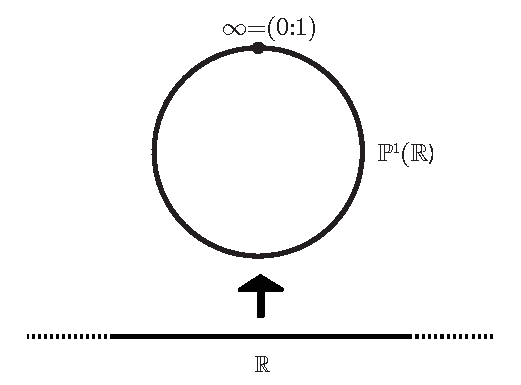
\includegraphics[trim=0cm 0cm 0cm 0cm,clip,scale=0.75]{images/projlinetocirc.pdf}
\end{minipage}
\vspace{-2mm}
\end{example}
\subsection{Chiusura proiettiva di un sottospazio affine}
\begin{define}\textsc{Chiusura proiettiva.}\\
	Sia $r\subseteq\aff{\kamp^n}$ una retta affine. La \textbf{chiusura proiettiva}\index{chiusura proiettiva}\index{chiusura!proiettiva} di $r$ è il sottospazio proiettivo $\overline{r}\subseteq\proj[n]{\ }$ generato da $r\subseteq U_0\subseteq\proj[n]{\ }$.
\end{define}
\begin{proposition}
	$\overline{r}$ è una \textit{retta proiettiva} e si ha:
	\begin{equation}
		\overline{r}=r\cup P_{\infty}
	\end{equation}
Dove $P_{\infty}=\overline{r}\cap H_0$ è detto \textit{punto all'infinito} o \textit{punto improprio} della retta $r$.
\end{proposition}
\begin{demonstration}
	Sia $v\in\kamp^n\setminus\left\{0\right\}$ la direzione di $r$ e $w\in r$ un punto della retta. Allora $r$ ha descrizione parametrica in $\aff{\kamp^n}$:
	\begin{equation*}
		\begin{cases}
			\begin{array}{l}
				X_1=tv_1+w_1\\
				\vdots\\
				X_n=tv_n+w_n\\			
			\end{array}
		\end{cases}\quad t\in\kamp
	\end{equation*}
Consideriamo la retta proiettiva $R\subseteq\proj[n]{\ }$ con descrizione parametrica:
\begin{equation*}
\begin{cases}
		\begin{array}{l}
			x_0=s\\
			x_1=tv_1+sw_1\\
			\vdots\\
			x_n=tv_n+sw_n\\			
		\end{array}
	\end{cases}\quad \left(s\colon t\right)\in\proj[1]{\ }
\end{equation*}
$R$ è la retta proiettiva per i punti:
\begin{equation*}
	t=0\ \colon\ \left(1\colon w_1\colon\ldots\colon w_n\right)\quad t=1\ \colon\ \left(0\colon v_1\colon\ldots\colon v_n\right)=P_\infty
\end{equation*}
Ponendo $s=1$ otteniamo:
\begin{equation*}
	\begin{cases}
		\begin{array}{l}
			x_0=1\\
			x_1=tv_1+w_1\\
			\vdots\\
			x_n=tv_n+w_n\\			
		\end{array}
	\end{cases}\quad t\in\kamp
\end{equation*}
Al variare di $t\in\kamp$, questi sono tutti e soli i punti di $j\left(r\right)\subseteq U_0\subseteq \proj[n]{\ }$. Si ha dunque che $R$ è una retta proiettiva contente $r$:
\begin{equation*}
	\begin{array}{ll}
			R&=r\cup P_{\infty}\\
			P_{\infty}&=R\cap H_0=\left\{\left(0\colon v_1\colon v_n\right)\right\}
	\end{array}
\end{equation*}
$R$ è necessariamente il più piccolo sottospazio proiettivo contenente $r$, dato che è la retta più un solo punto. Pertanto, $R=\overline{r}$.
\end{demonstration}
\begin{observes}~{}
	\begin{enumerate}
		\item Il punto improprio di $r$ è:
		\begin{equation*}
			P_{\infty}=\left(0\colon v_1\colon \ldots\colon v_n\right)
		\end{equation*}
	E corrisponde esattamente alla \textit{direzione} $v=\left(v_1,\ \ldots,\ v_n\right)$ di $r$.
	Poiché $P_\infty=\left[v\right]$ con $v$ la direzione di $r$, ne segue che l'iperpiano improprio di $\proj[n]{\kamp }$ è:
	 \begin{equation*}
		\begin{array}{ll}
			H_0 & =\proj[n-1]{\kamp}=\proj{\kamp^n}=\left\{\text{rette vettoriali in }\kamp^n\right\}=\\
			&=\left\{\text{direzioni delle rette affini in }\aff{\kamp^n}\right\}
		\end{array}
	\end{equation*}
\item Due rette affini $r_1,\ r_2\subseteq \aff{\kamp^n}$ hanno lo stesso punto improprio se e solo hanno la \textit{stessa direzione}, cioè se sono \textit{parallele}.\\
Se $r_1\neq r_2$ e $r_1$ e $r_2$ sono parallele, allora $r_1\cap r_2=\emptyset$ in $\aff{\kamp^n}$, ma $\overline{r_1}\cap \overline{r_2}={P_{\infty}}$ in $\proj[n]{\ }$. Ciò ci porta a dire che due rette parallele $r_1$ e $r_2$ si incontrano sempre all'\textit{infinito}!
\item Se $n=2$, cioè operando in $\proj[2]{\ }$, due rette distinte $r_1,\ r_2\subseteq \aff{\kamp^2}$ sono o \textit{incidenti} o \textit{parallele}, ma in $\proj[2]{\ }$ si intersecano sempre.
\item Viceversa: sia $l\subseteq \proj[n]{\ }$ una retta proiettiva. Abbiamo due casi:
\begin{itemize}
	\item $l\subseteq H_0,\ l\cap U_0= \emptyset$.
	\item $l\nsubseteq H_0\implies l+H_0=\proj[n]{\ }$.
\end{itemize}
Infatti, si ha che $l+H_0$ è un sottospazio proiettivo che contiene strettamente $H_0$, dato che $l\nsubseteq H_0$, e usando la formula di Grassmann otteniamo:
\begin{equation*}
	\dim\left(l+H_0\right)=\dim l +\dim H_0-\dim \left(l\cap H_0\right)=1+n-1+0=n=\dim \proj[n]{\ }\implies l+H_0 = \proj[n]{\ }
\end{equation*}
Sempre dalla formula di Grassmann:
\begin{equation*}
	\dim\left(l\cap H_0\right)=0\implies l\cap H_0=\left\{1 \text{punto}\right\}=\left\{Q\right\}
\end{equation*}
Cioè $l\cap U_0=l\setminus\left\{Q\right\}$. In altre parole, $l$ è una retta affine in $\aff{\kamp^n}$ con un \textit{punto improprio} $Q$ e necessariamente $l$ è la chiusura proiettiva di $l\setminus\left\{Q\right\}$.
\item Sia $n=2$, cioè operiamo in $\proj[2]{\ }$. Una retta $r\subseteq \aff{\kamp^2}$ è descritta da un'equazione lineare:
\begin{equation}
	ax+by+c=0\quad \left(a,\ b\right)\neq\left(0,\ 0\right)
\end{equation}
Con la corrispondenza biunivoca fra le coordinate $\left(x,\ y\right)$ vettoriali e $\left(X_1,\ X_2\right)$ affini. Abbiamo tuttavia anche la corrispondenza con le coordinate omogenee in $\proj[2]{\ }$, rispettivamente $\left(x\colon y\colon z\right)$ e $\left(_0\colon x_2\colon x_3\right)$.\\
Chiamiamo $\left(x\colon y\colon z\right)$ le coordinate omogenee su $\proj[2]{\ }$ con:
\begin{equation*}
	H_0=\left\{P=\left(x\colon y\colon z\right)\in \proj[2]{\ }\mid z=0\right\}=\left\{P=\left(x\colon y\colon0\right)\in \proj[2]{\ }\right\}
\end{equation*}
Allora la chiusura proiettiva $\overline{r}\subseteq \proj[2]{\ }$ di $r$ ha in $\proj[2]{\ }$ l'equazione lineare omogenea seguente:
\begin{equation}
		ax+by+cz=0
\end{equation}
Infatti, per $z=1$ si ottiene l'equazione di $r$, mentre ponendo $z=0$ (cioè il passaggio per $H_0$) troviamo il punto improprio $P_{\infty}$ di $r$:
\begin{equation*}
		\begin{cases}
		\begin{array}{l}
			z=0\\
			ax+by=0\\	
		\end{array}
	\end{cases}\quad P_{\infty}=\left(-b\colon a\colon 0\right)
\end{equation*}
La direzione della retta $ax+by+c=0$ è data dal punto improprio $P_{\infty}$ e corrisponde al vettore $\left(-b, a\colon 0\right)$.
	\end{enumerate}
\end{observes}
Generalizziamo ora il concetto di chiusura proiettiva a un generico sottospazio affine.
\begin{define}\textsc{Chiusura proiettiva di un sottospazio}.\\
	Dato $S\subseteq \aff{\kamp^n}$ un sottospazio affine con $S\neq \emptyset$, la \textbf{chiusura proiettiva}\index{chiusura!proiettiva} $\overline{S}\subseteq \proj[n]{\ }$ di $S$ è il sottospazio proiettivo generato da $S$. Esso ha dimensione $\dim \overline{S}=\dim S=m$.
\end{define}
\textbf{Equazioni cartesiane}. Se $S$ come sottospazio affine è dato in forma cartesiana dal sistema lineare $h\times\left(n+1\right)$ seguente:
\begin{gather*}
			Ax+b=0\qquad\left(\begin{array}{c}
		X_1\\
		\vdots\\
		X_n
	\end{array}\right)\in\aff{\kamp^{n}}\\
	\begin{cases}
	\begin{array}{l}
		a_{1,1}X_1+\ldots+a_{1,n}X_n+b_1=0\\
		\vdots\\
		a_{h,1}X_1+\ldots+a_{h,n}X_n+b_h=0\\			
	\end{array}
\end{cases}
\end{gather*} 
Allora $\overline{S}$ è descritto dal sistema lineare omogeneo  $h\times\left(n+1\right)$ in $\left(x_0,\ \ldots,\ x_n\right)$ seguente:
\begin{gather*}
	\left(A\mid b\right)x=0\qquad\left(\begin{array}{c}
		x_1\\
		\vdots\\
		x_n\\
		x_0
	\end{array}\right)\in\proj[n]{\ }\\
	\textcolor{red}{\circled{\ast}}\begin{cases}
		\begin{array}{l}
			a_{1,1}x_1+\ldots+a_{1,n}x_n+b_1x_0=0\\
			\vdots\\
			a_{h,1}x_1+\ldots+a_{h,n}x_n+b_hx_0=0\\			
		\end{array}
	\end{cases}
\end{gather*}
\begin{demonstration}
	Studiamo le dimensioni di $S$ e $\overline{S}$ usando i sistemi cartesiani appena definiti:
	\begin{equation*}
		\begin{array}{l}
			\dim S=\dim \kamp^n-\rk\left(A\right)=n-\rk\left(A\right)\\
			\dim \overline{S}=\dim \proj[n]{\ }-\rk\left(A\mid b\right)-1=\left(n+1-\rk\left(A\mid b\right)\right)-1=n-\rk\left(A\mid b\right)\\
		\end{array}
	\end{equation*}
	Per Rouché-Capelli vale $\rk A=\rk \left(A\mid b\right)$ in quanto $S\neq \emptyset$. In questo modo abbiamo dimostrato che $\dim \overline{S}=\dim S$.
\end{demonstration}
I \textit{punti impropri} del sottospazio affine $S$ sono dati da $\overline{S}\cap H_0$, con $\overline{S}$ la chiusura proiettiva di $S$ e $H_0$ l'iperpiano improprio. Dal sistema $\textcolor{red}{\circled{\ast}}$ si ha che $\overline{S}\cap H_0$ è dato da:
\begin{equation*}
	\begin{cases}
		\begin{array}{l}
			x_0=0\\
			a_{1,1}x_1+\ldots+a_{1,n}x_n=0\\
			\vdots\\
			a_{h,1}x_1+\ldots+a_{h,n}x_n=0\\			
		\end{array}
	\end{cases}
\end{equation*}
Esso corrisponde al sistema lineare omogeneo in $\kamp^n$ $Ax=0$ associato al sistema lineare $Ax+b=0$ che definisce $S$. In altre parole, $\overline{S}\cap H_0$ corrisponde al \textit{sottospazio vettoriale direttore} $W\subseteq \kamp^n$ e vale $\overline{S}\cap H_0=\proj{W}$ direzione di $S$. La sua dimensione per definizione di direzione è:
\begin{equation*}
	\dim\left(\overline{S}\cap H_0\right)=\dim S-1=\dim\overline{S}-1
\end{equation*}
\textbf{Equazioni parametriche}. Se $S$ ($\dim S=m$) è data in \textit{forma parametrica} e il sottospazio direttore $W\subseteq \kamp^n$ ha una base $\left\{v_1,\ \ldots,\ v_m\right\}$ (tali che $v_i=\left(V_{i,1},\ \ldots,\ V_{i,n}\right)\in\aff{\kamp^n}$ per un dato sistema di riferimento affine), posto $c\in S$ ricordiamo che l'espressione parametrica di $S$ è:
\begin{gather*}
	X=t_1v_1+\ldots+t_mv_m+c\quad t_1,\ \ldots,\ t_m\in\kamp\\
		\begin{cases}
		\begin{array}{l}
			X_1=t_1V_{1,1}+\ldots+t_mV_{m,1}+C_1\\
			\vdots\\
			X_n=t_1V_{1,n}+\ldots+t_mV_{m,n}+C_n\\			
		\end{array}
	\end{cases}
\end{gather*}
Allora, $\overline{S}$ è il sottospazio generato dagli $m+1$ punti \textit{indipendenti}:
\begin{equation}
	\begin{array}{cc}
		\left(0\colon v_{i,1}\colon\ldots\colon v_{in}\right)&i=1,\ \ldots,\ m
		\left(1\colon c_1\colon\ldots\colon c_n\right)
	\end{array}
\end{equation}
Pertanto, $\overline{S}$ ha descrizione parametrica:
\begin{equation*}
			\begin{cases}
		\begin{array}{l}
			x_0=t_0\\
			x_1=t_1v_{1,1}+\ldots+t_mv_{m,1}+t_0C_1\\
			\vdots\\
			x_n=t_1v_{1,n}+\ldots+t_mv_{m,n}+t_0C_n\\			
		\end{array}
	\end{cases}
\end{equation*}
Con $\left(t_0\colon\ldots\colon t_m\right)\in\proj[m]{\ }$.
\subsection{Un esempio di proiettività}
Vediamo un esempio di proiettività di $\proj[1]{\ }$.
\begin{example}
	Si consideri $\proj[1]{\kamp} = \aff{\kamp} \cup \{\infty\}$ con $\infty=(0\colon 1)$. Sia $\funz f {\proj[1]{\ }} {\proj[1]{\ }}$ una proiettività (dunque \textit{biunivoca}) definita come $f(x_0\colon x_1)=(ax_0+bx_1\colon cx_0+dx_1)$. Si ha che $f(0\colon 1)=(b\colon d)$, mentre la sua controimmagine è $f(-b\colon a)=(0\colon 1)$; infatti, siccome le coordinate sono omogenee, basta porre $ax_0+bx_1=0$.\newline
	Sia $t=\frac{x_1}{x_0}$ la coordinata affine su $\aff{\kamp}$. Se $x_0\neq 0$, tutti i punti $(x_0\colon x_1)$ si possono scrivere come $(x_0\colon x_1)=\left( 1\colon \frac{x_1}{x_0} \right)=(1\colon t)$, che corrispondono al punto $t\in\kamp$. Vediamo ora come si comporta l'immagine grazie a queste osservazioni se $ax_0+bx_1\neq 0$:
	\begin{gather*}
		f(x_0\colon x_1)=(ax_0+bx_1\colon cx_0+dx_1)= \left(1\colon \frac{cx_0+dx_1}{ax_0+bx_1} \right)  =  \left( 1 \colon  \frac{ x_0 \left( c+ d \frac{x_1}{x_0} \right) }{ x_0 \left( a+ b\frac{ x_1 }{ x_0 } \right)} \right)=\left( 1\colon \frac{dt+c}{bt+a}\right)
	\end{gather*}
	Dunque la proiettività $f$ corrisponde alla trasformazione $\funz F {\kamp\cup \{\infty\}} {\kamp\cup \{\infty\}}$ con $F(t)=\begin{cases}
		\frac{dt+c}{bt+a}, & t\in\kamp, \ t\neq -\frac{a}{b}\\
		\infty, & t=-\frac{a}{b}\\
		\frac{d}{b}, & t=\infty
	\end{cases}$
	dove per $t=-\frac{a}{b}$ si ottiene $f(-b\colon a)=(0\colon 1)=\infty$. La prima equazione è detta \textit{trasformazione lineare fratta}, che è definita sulla retta affine tranne dove si annulla il denominatore. \newline
	Notiamo che $F$ diventa un'affinità $\funztot{F}{\aff{\kamp}} {\aff{\kamp}}{t}{\alpha t+\beta}$ se e solo se il denominatore diventa una costante ponendo $b=0$, cioè se è della forma $F(t)=\alpha$.
	Ciò significa che la proiettività fissa il punto all'infinito ($f(0\colon 1)=(0\colon 1)$), mentre la parte affine viene mandata in sè stessa.\newline
	Questo ragionamento si può vedere anche in dimensione superiore.
\end{example}
\subsection{Impratichiamoci! Geometria affine e geometria proiettiva}
\begin{exercise}
	Sia $\kamp=\realset$. Allora, preso $\realset^n$ con la topologia euclidea e $\proj[n]{\realset}$ con la topologia quoziente, mostrare che $U_0$ è un aperto di $\proj[n]{\realset}$ e che $\funz{j}{\realset^n}{U_0}$ è un omeomorfismo.
\end{exercise}
\begin{solution}
	... % aggiungere soluzione
\end{solution}

%LEZ 31 
\section{Spazi proiettivi complessi}
%Digressione di topologia sugli spazi proiettivi complessi
\begin{remember}
	Nel caso di $\realset^n$ si è già visto che lo spazio proiettivo reale è un quoziente del tipo $\displaystyle \proj[n]{\realset}=\frac{\realset^{n+1}\setminus\{0\}}{\sim}$, dunque è dotato in maniera naturale di una topologia.\newline
	Si può anche vedere come \textit{quoziente della sfera} $S^n$ dove si identificano i punti antipodali grazie alla \textit{suriezione} $\surr \pi {S^n} {\proj[n]{\realset}}$; è anche una \textit{varietà topologica compatta} di dimensione $n$. Inoltre $\proj[1]{\realset}\cong S^1$ e abbiamo analizzato il piano proiettivo reale $\proj[2]{\realset}$.
\end{remember}
Anche nel caso complesso per $\proj[n]{\complexset}=\frac{\complexset^{n+1}\setminus\{0\}}{\sim}$ si ha in maniera naturale una topologia quoziente data dalla topologia euclidea su $\complexset^{n+1}\setminus\{0\} \cong \realset^{n+1}\setminus\{0\}$.\newline
Vogliamo vedere che è una \textit{varietà topologica compatta} di dimensione $\mathbf{2n}$. Infatti, mentre $\proj[n]{\realset}$ è localmente euclideo di dimensione $n$, si ha che $\proj[n]{\complexset}$ localmente si comporta come $\complexset^n\cong\realset^{2n}$, dunque la dimensione topologica è $2n$.
\begin{theorema}
	$\proj[n]{\complexset}$ è una varietà topologica di dimensione $2n$.
\end{theorema}
\begin{demonstration}~{}
	\begin{itemize}
		\item $\proj[n]{\complexset}$ è \textbf{connesso}: è quoziente di $\complexset^{n+1}\setminus\{0\}$, che è connesso.
		\item $\proj[n]{\complexset}$ è \textbf{compatto}: per avere la tesi, si vuole vedere lo spazio come \textit{quoziente di un compatto} o \textit{immagine tramite una funzione continua di un compatto}. 
		Ricordiamo la relazione di equivalenza:
		\begin{equation*}
			z\sim w\iff \exists\lambda\in\complexset\setminus\{0\}\colon w=\lambda z
		\end{equation*}
		Vogliamo ora \textit{restringerci alla sfera complessa} (la cui dimensione è data da $\complexset^{n+1}=\realset^{2n+2}\supset S^{2n+1}$) e dimostrare che ogni \textit{punto del quoziente} è equivalente ad un \textit{punto della sfera}. Per fare ciò si sfrutta la corrispondenza fra numeri complessi e reali e la norma:
		\begin{gather*}
			z_j=x_j+iy_j\implies  z=(z_1,\ \ldots,\ z_{n+1})\in\complexset^{n+1}\longleftrightarrow (x_1,\ y_1,\ \ldots,\ x_{n+1},\ y_{n+1})\in\realset^{2n+2}\\
			\begin{array}{ccc}
				\displaystyle \|z\|^2=\sum_{j=1}^{n+1} \lvert z_j\rvert ^2=\sum_{j=1}^{n+1}\left(\lvert x_j \rvert ^2 +\lvert y_j \rvert ^2\right) & \wedge & \displaystyle \ \|\lambda z \| =\sqrt{\sum_{j=1}^{n+1}\lvert \lambda z_j \rvert ^2}=\lvert\lambda\rvert \| z\|,\ \lambda\in\complexset
			\end{array}
		\end{gather*}
	 Se $z\in\complexset^{n+1}\setminus\{0\}\implies \|z\|\neq 0$ e se $\lambda=\frac{1}{\| z\|}$ si ha $\underbrace{\frac{1}{\|z\|}\cdot z}_{\in S^{2n+1}}\sim z$. Notiamo allora che $\pi(S^{2n+1})=\proj[n]{\complexset}$, dunque $\proj[n]{\complexset}$ è compatto.
	\item $\proj[n]{\complexset}$ è di \textbf{Hausdorff}: partiamo con una considerazione che segue dal punto precedente. Nel caso reale, i punti sulla sfera sono equivalenti solo se \textit{antipodali}, nel caso complesso $S^{2n+1}$ invece si ha, dati $z,w\in S^{2n+1}$:
		\begin{equation*}
			z\sim w\iff \exists \lambda\in\complexset\setminus\{0\} \colon w=\lambda z
		\end{equation*}
	Siccome $w,z\in S^{2n+1}$ hanno norma unitaria $1=\| w\|=\|\lambda z\|= \ \lambda | \|z\|=|\lambda|$. Essendoci \textit{infiniti} numeri di norma $1$ in $\complexset$, allora ci sono \textit{infiniti} numeri nella stessa classe, e quindi i punti $\lambda z\in S^{2n+1}$ sono tutti equivalenti.\\
	Consideriamo ora $\funz{\pi_0=\pi_{\mid S^{2n+1}}}{S^{2n+1}}{\proj[n]{\complexset}}$. Per dimostrare che $\proj[n]{\complexset}$ è di Hausdorff, è sufficiente dimostrare che $\pi_0$ sia una identificazione chiusa: in questo modo, per il teorema % Y hausdorff iff f identificazione chiusa se X compatto + Hausdorff e f identificazione.
	basta dimostrare che $\pi_0$ è un'identificazione \textit{chiusa}.\\
	Sia $C\subset S^{2n+1}$ un chiuso. Allora $\pi_0(C)$ è chiuso in $\proj[n]{\complexset}\iff \pi_0^{-1}(\pi_0(C))$ è chiuso in $S^{2n+1}$.
	Notiamo che:
	\begin{equation*}
		\pi_0\left(z\right)\sim \pi_0\left(w\right)\iff \exists\lambda\in\complexset\text{ con }\lvert\lambda\rvert=1\colon w=\lambda z
	\end{equation*}
	In effetti la relazione di equivalenza su $S^{2n+1}$ viene da un'azione del gruppo $S^1=\{\lambda\in\complexset \mid |\lambda |=1\}$ rispetto al prodotto con elemento neutro $1$:
	\begin{equation*}
		\funztot F {S^1\times S^{2n+1}} {S^{2n+1}} {(\lambda, z)} {\lambda z}
	\end{equation*}
	\begin{itemize}
		\item $F$ è un'applicazione continua.
		\item $S^1\times S^{2n+1}$ è compatto e \textbf{Hausdorff}.
	\end{itemize}
	$F$ è \textit{chiusa} in quanto funzione continua da un compatto in \textbf{Hausdorff}.\\
	Dato un chiuso $C\subseteq S^{2n+1}$, prendendo la controimmagine dell'immagine agisco sui punti di $C$ con tutti gli elementi di $S^1$, cioè prendo tutte le orbite che intersecano $C$, ottenendo quanto segue:
	\begin{equation*}
		\pi_0^{-1}(\pi_0(C))=F(\underbrace{S^1\times C}_{\stackrel{\text{chiuso in}}{S^1\times S^{2n+1}}})\subseteq S^{2n+1}
	\end{equation*}
\vspace{-1mm}
Segue che $\pi_0^{-1}(\pi_0(C))$ chiuso  e $\pi_0(C)$ chiuso in $\proj[n]{\complexset}$, cioè $\pi_0$ è applicazione chiusa e $\pi_0$ identificazione per il teorema % manetti 5.4
.\\
Pertanto $\proj[n]{\complexset}$ è anche quoziente di $S^{2n+1}$.
Siccome $S^{2n+1}$ è un compatto in un \textbf{Hausdorff} per 
%AAA ESERCIZIO TUTORATO QUOZIENTE CERCASI	
		e siccome $\pi_0$ è un'identificazione \textit{chiusa} allora $\proj[n]{\complexset}$ è \textbf{Hausdorff} per il teorema già citato in precedenza.
		\item $\proj[n]{\complexset}$ è \textbf{localmente euclideo di dimensione} $2n$: per dimostrarlo sfruttiamo la costruzione
%AAA COSTRUZIONE CERCASI NELLA SCORSA LEZIONE
		. Consideriamo la famiglia di insiemi:
		\begin{equation*}
			U_j\coloneqq\{z_j\neq 0\}=\proj[n]{\complexset}\setminus H_j\text{, con }H_j\ j\text{-esimo iperpiano coordinato.}
		\end{equation*}
		Per semplicità sia $j=0$.\newline 
		Si consideri la proiezione al quoziente $\funz \pi {\complexset^{n+1}\setminus\{0\}} {\proj[n]{\complexset}}$ e la controimmagine $\pi^{-1}(U_0)=\{z\in\complexset^{n+1}\setminus\{0\}\mid z_0\neq 0\}$, aperto in $\complexset^{n+1}\setminus\{0\}$ in quanto abbiamo tolto un iperpiano. Segue che $U_0$ è aperto in $\proj[n]{\complexset}$ e lo stesso vale per tutti gli $U_j$. Ricordando la costruzione 
	%AAA COSTRUZIONE DI J E \PHI CERCASI
		si considerano le seguenti mappe biunivoche, una inversa dell'altra: 
		\begin{equation*}
			\funztot j {\complexset^n} {U_0} {(z_1,\ \ldots,\ z_n)} {(1\colon z_1\colon \ldots\colon z_n)}\quad \funztot \oldphi {U_0} {\complexset^n} {(z_0\colon\ldots\colon z_n)} {\left( \frac{z_1}{z_0},\ \ldots,\ \frac{z_n}{z_0} \right)}
		\end{equation*}
		Mostriamo che $j$ e $\oldphi$ siano omeomorfismi; siccome sono già biunivoche e una inversa dell'altra basta dimostrare che sono entrambe \textit{continue}.\\
			\begin{minipage}[t]{0.51\textwidth}\vspace{1pt}
				Per mostrare che $j$ è continua sfruttiamo il diagramma a lato, ovvero la fattorizzazione di $j$ in $\complexset^{n+1}\setminus\{0\}$ tramite:
					\begin{equation*}
						\widetilde{j}((z_1,\ \ldots,\ z_n))=(1,\ z_1\ldots,\ z_n)
					\end{equation*}
				E la proiezione $\pi$, che in questo caso opera nel seguente modo:
					\begin{equation*}
					\pi((1,\ z_1\ \ldots,\ z_n))=(1\colon z_1\colon\ldots\colon z_n)
				\end{equation*}
				 Siccome $\widetilde{j}$ e $\pi$ sono continue, allora anche la loro composizione $j$ lo è.
			\end{minipage}\hspace{-15pt}
			\begin{minipage}[t]{0.49\textwidth}\vspace{25pt}
				% https://q.uiver.app/?q=WzAsNCxbMSwwLCJcXGNvbXBsZXhzZXRee24rMX1cXHNldG1pbnVzXFx7MFxcfSJdLFswLDIsIlxcY29tcGxleHNldF5uIl0sWzIsMiwiVV8wIl0sWzEsMl0sWzEsMCwiXFx3aWRldGlsZGV7an0iXSxbMSwyLCJqIiwyXSxbMCwyLCJcXHBpIl1d
				\[\begin{tikzcd}
					& {\complexset^{n+1}\setminus\{0\}} \\
					\\
					{\complexset^n} & {} & {U_0}
					\arrow["{\widetilde{j}}", from=3-1, to=1-2]
					\arrow["{j}"', from=3-1, to=3-3]
					\arrow["{\pi}", from=1-2, to=3-3]
				\end{tikzcd}\]
			\end{minipage}\\
			\begin{minipage}[t]{0.51\textwidth}\vspace{10pt}
				Per la continuità dell'inversa $\oldphi$ si procede con la fattorizzazione della controimmagine $\pi^{-1}$ tramite una restrizione dell'inversa di $\pi$ a $\pi^{-1}U_0$:
				\begin{equation*}
					\funz {p\coloneqq \pi_{|_{\pi^{-1}(U_0)}}} {\pi^{-1}(U_0)} {U_0}
				\end{equation*}
				E tramite $\hat{\oldphi}$:
				\begin{equation*}
					\widehat{\oldphi}(z_0,\ \ldots,\  z_n)=\left( \frac{z_1}{z_0},\ \ldots,\ \frac{z_n}{z_0}\right)
				\end{equation*}
			\end{minipage}\hspace{-15pt}
			\begin{minipage}[t]{0.49\textwidth}\hspace{-15pt}\vspace{25pt}
				% https://q.uiver.app/?q=WzAsNCxbMiwwLCJcXHBpXnstMX0oVV8wKSJdLFszLDAsIlxcc3Vic2V0IFxcY29tcGxleHNldF57fW4rMSJdLFswLDIsIlVfMCJdLFszLDIsIlxcY29tcGxleHNldF5uIl0sWzIsMywiXFxvbGRwaGkiLDJdLFswLDIsInAiLDJdLFswLDMsIlxcaGF0e1xcb2xkcGhpfSJdXQ==
				\[\begin{tikzcd}
					&[-35pt]& {\pi^{-1}(U_0)}\subset \complexset^{n+1} &[-15pt] {} \\
					\\
					{U_0} &&& {\complexset^n}
					\arrow["{\oldphi}"', from=3-1, to=3-4]
					\arrow["{p}"', from=1-3, to=3-1]
					\arrow["{\widehat{\oldphi}}", from=1-3, to=3-4]
				\end{tikzcd}\]
			\end{minipage}\\
		 Entrambe sono \textit{continue}: la prima è la restrizione di una funzione continua e la seconda, essendo ben definita ($U_0=\{z_0\neq 0\}$), risulta banalmente continua: inoltre, quest'ultima lavora solo con vettori e non con classi di equivalenza!\\
		Per dimostrare che $\oldphi$ è continua sfruttiamo le proprietà della topologia quoziente (vedasi \ref{proprietà identificazione quoziente e mappa continua indotta}), dimostrando che $p$ è un'\textit{identificazione}: è già \textit{continua} e \textit{suriettiva}, dunque basta solo che sia aperta o chiusa per il teorema \ref{condizione sufficiente identificazione}.\\
		Osserviamo che $\funz \pi {\complexset^{n+1}\setminus\{0\}} {\proj[n]{\complexset}}$ è anch'essa un quoziente dato dall'azione del gruppo \footnote{Questo vale in generale per gli spazi proiettivi, si veda 
%AAA ESERCIZIO GIà DATO CERCASI	
		.} $G=\complexset\setminus\{0\}$ rispetto al prodotto per la moltiplicazione su $\complexset^{n+1}\setminus\{0\}$. In particolare, è un'azione per omeomorfismi. Infatti, fissato  $\lambda\in\complexset\setminus\{0\}$:
	\begin{equation*}
		\funztot {\theta_\lambda} {\complexset^{n+1}\setminus\{0\}} {\complexset^{n+1}\setminus\{0\}} z {\lambda z}
	\end{equation*}
	È continua: per la proposizione \ref{proiezione azione gruppo aperta} si ha che $\funz \pi {\complexset^{n+1}\setminus\{0\}} {\proj[n]{\complexset}}$ è un'applicazione aperta, pertanto anche $p$ che è una sua restrizione ad un aperto è aperta %(verifica per esercizio)
	. Dalle considerazioni di cui sopra $p$ è un'identificazione. Ne segue che $U_0$ è un aperto di $\proj[n]{\complexset}$ omeomorfo a $\complexset^n$ e quindi a $\realset^{2n}$.\\
	Allo stesso modo, $\forall j\in\{0,\ \ldots,\ n\},\ U_j$ è un aperto di $\proj[n]{\complexset}$ omeomorfo a $\complexset^n$ tramite la mappa-.
	\begin{equation*}
		\funztot {\oldphi_j} {U_j} {\complexset^n} {(z_0\colon\ldots\colon z_n)} {\left( \frac{z_0}{z_j},\ldots,\frac{z_{j-1}}{z_j}, \frac{z_{j+1}}{z_j},\ldots, \frac{z_n}{z_j} \right)}
	\end{equation*}
	Siccome in \textit{coordinate omogenee} c'è sempre un elemento \textit{non} nullo (si lavora su $\complexset^{n+1}\setminus\{0\}$) allora ogni punto sta in uno degli aperti $U_j$, cioè:
	\begin{equation*}
		\proj[n]{\complexset}=U_0\cup\ldots\cup U_n\implies \proj[n]{\complexset}
	\end{equation*}
	 $\proj[n]{\complexset}$ è \textit{localmente euclideo} di dimensione $2n$, dunque è una \textit{varietà topologica compatta}.
	\end{itemize}
\vspace{-3mm}
\end{demonstration}
\begin{observes}~{}
	\begin{itemize}
		\item Su un campo $\kamp$ qualsiasi si ha sempre la mappa $\oldphi_j$, una corrispondenza biunivoca fra i sottoinsiemi $U_j$ (complementari di un iperpiano coordinato) e $\kamp^n$ (senza aspetto topologico): vale sempre che lo spazio proiettivo è unione di tali $U_j$.\\
		In particolare, nel caso reale, tali $U_j$ sono \textit{aperti} ed il ragionamento è \textit{analogo} a quello fatto poc'anzi nel caso complesso.
		\item Non abbiamo dimostrato che è a base numerabile perché essendo compatto segue dal teorema
%AAA TEOREMA SUPERFICI COMPATTE CERCASI
		, inoltre si potrebbe dimostrare facilmente "a mano" sfruttando che gli aperti $U_j$ sono a base numerabile, dunque anche la loro unione finita lo è.
	\end{itemize}
\vspace{-3mm}
\end{observes}

	\subsection{Retta proiettiva complessa}
Cosa succede per la \textit{retta proiettiva complessa}? Essa è una varietà topologica compatta di dimensione $2$ (dunque una \textit{superficie topologica compatta}) che abbiamo già classificato! Scopriamo di che superficie si tratta.
%AAA MOTIVAZIONE CERCASI
Si ha:
\begin{equation}
	\proj[n]{\complexset}=U_0\cup\{(0\colon 1)\}\text{ con } U_0\cong\complexset\cong\realset^2
\end{equation}
In altre parole, la retta proiettiva complessa è un \textit{piano} unito ad un \textit{punto}. Dimostriamo ora che è omeomorfa a $S^2$, detta anche \textbf{sfera di Riemann} \index{sfera!di Riemann}, e analizziamo poi la differenza con il piano proiettivo reale.
\begin{theorema}
	$\proj[1]{\complexset}\cong S^2$
\end{theorema}
\begin{intuit}
	Per ottenere la sfera si può pensare di \textit{richiudere} il piano $\realset^2$ su se stesso, aggiungendo il punto all'infinito $\{(0\colon 1)\}$.
\end{intuit}
\begin{demonstration}
	Costruiamo l'omeomorfismo con $S^2\subset\realset^3$ sfruttando la \textit{proiezione stereografica}. % \funz F {S^2} {\proj[1]{\complexset}}$ prima sulla restrizione della sfera senza il polo nord $N=(0,0,1)$ e poi la estendiamo anche in $N$.
	Consideriamo:
		% https://q.uiver.app/?q=WzAsNCxbMCwwLCJTXjJcXHNldG1pbnVzXFx7TlxcfSJdLFsyLDAsIlxccmVhbHNldF4yIl0sWzQsMCwiXFxjb21wbGV4c2V0Il0sWzYsMCwiVV8wIl0sWzAsMSwicF9OIl0sWzEsMiwiayJdLFsyLDMsImoiXSxbMCwzLCJGX3t8X3tTXjJcXHNldG1pbnVzXFx7TlxcfX19IiwyLHsiY3VydmUiOjV9XV0=
		\[\begin{tikzcd}
			{S^2\setminus\{N\}} && {\realset^2} && {\complexset} && {U_0}
			\arrow["{p_N}", from=1-1, to=1-3]
			\arrow["{k}", from=1-3, to=1-5]
			\arrow["{j}", from=1-5, to=1-7]
			\arrow["{F_{|_{S^2\setminus\{N\}}}}"', from=1-1, to=1-7, curve={height=30pt}]
		\end{tikzcd}\]
	Con $\funz {p_N} {S^2\setminus\{N\}} {\realset^2}$ la \textit{proiezione stereografica} dal polo nord $N=(0,\ 0,\ 1)$, $\funztot k {\realset^2} \complexset {(x,\ y)} {x+iy}$ e $\funztot j \complexset {U_0} w {(1\colon w)}$. Allora definiamo una funzione $F$ su $S^2\setminus\{N\}$:
	\begin{equation*}
		F_{\mid_{S^2\setminus\{N\}}}\coloneqq j\circ k\circ p
	\end{equation*}
	Poniamo $F(N)\coloneqq (0\colon 1)$ in quanto sono gli unici punti rimasti da dover ‘‘mappare'', ricordando che $\proj[1]{\complexset}=U_0\cup\{(0\colon 1)\}$. \\
	Siccome $j\ ,\ k,\ p$ sono \textit{tutti} omeomorfismi, allora la loro composizione $F_{\mid_{S^2\setminus\{N\}}}$ è biunivoca e continua su $S^2\setminus\{N\}$.\\
	Perché $F$ sia continua in tutti i suoi punti basta verificarla che lo sia in un intorno (aperto) contenente $N$. % per il manetti, 3.27 ?
	Sfruttiamo la proiezione stereografica dal polo sud $S=(0,\ 0,\ -1)$ scegliamo l'aperto $S^2\setminus\{S\}$, intorno di $N$. Dobbiamo mostrare la continuità di $F_{\mid_{S^2\setminus\{S\}}}$.\\
	Scriviamo le due proiezioni stereografiche, sia da $N$, sia da $S$: fissato un punto $P_0=(x_0,\ y_0,\ z_0)$ sulla sfera, allora consideriamo le semirette uscenti da $N$ e da $S$ che passano per $P_0$ \footnote{Le equazioni sono scritte in \textit{forma parametrica}, pertanto abbiamo evidenziato il punto per cui passano e la direzione.}:
		\begin{gather*}
			\begin{array}{ccc}
				NP_0\colon \begin{cases}
					x=0+tx_0\\
					y=0+ty_0\\
					z=1+t(z_0-1)
				\end{cases}\quad P_0-N & \quad & SP_0\colon \begin{cases}
					x=0+tx_0\\
					y=0+ty_0\\
					z=-1+t(z_0+1)
				\end{cases}\quad P_0-S
			\end{array}
		\end{gather*}
	Per trovare le immagini delle proiezioni stereografiche intersechiamo le due semirette con il piano $xy$, cioè poniamo $z=0$:
		\begin{gather*}
			\begin{array}{ccc}
				N\ \colon  1+t(z_0-1)=0\implies t=\frac{1}{1-z_0} & \quad & S\ \colon -1+t(z_0+1)=0\implies t=\frac{1}{1+z_0}
			\end{array}
		\end{gather*}
	Notiamo che i denominatori non si annullano in entrambi i casi per la definizione delle proiezioni stereografiche sulla sfera meno $N$ ed $S$ rispettivamente.\\
	Ne segue che l'immagine di $\realset^2$ tramite la mappa standard $k$ è:
		\begin{gather*}
			\begin{array}{ccc}
				N\ \colon  \left( \frac{x_0}{1-z_0}, \frac{y_0}{1-z_0} \right) \mapsto w=\frac{x_0}{1-z_0} + i\frac{y_0}{1-z_0} \in\complexset & \quad &  S\ \colon \left( \frac{x_0}{1+z_0}, \frac{y_0}{1+z_0} \right) \mapsto u=\frac{x_0}{1+z_0} + i\frac{y_0}{1+z_0} \in\complexset
			\end{array}
		\end{gather*}
	Si ha che $w=\frac{1}{\overline{u}}$ e, viceversa, $u=\frac{1}{\overline{w}}$; infatti, quando $P_0\in S^2\setminus\{N,S\}$ allora $w,\ u\in\complexset\setminus\{0\}$. Verifichiamolo usando le proprietà dei numeri complessi:
		\begin{gather*}
			\frac{1}{\overline{u}} = \frac{1}{ \frac{x_0}{1+z_0} -i\frac{y_0}{1+z_0} } = \frac{1+z_0}{x_0-iy_0} \stackrel{!}{=} \frac{(x_0+iy_0)(1+z_0)}{x_0^2+y_0^2} \stackrel{!!}{=} \frac{(x_0+iy_0)(1+z_0)}{1-z_0^2}=\frac{x_0+iy_0}{1-z_0}=w
		\end{gather*}
	dove l'uguaglianza (!) vale perché, in quanto $P_0\neq N,\ S$ allora $x_0+iy_0\neq 0$, mentre quella (!!) segue dal fatto che il punto sta sulla sfera, per cui $x_0^2+y_0^2+z_0^2=1\implies x_0^2+y_0^2=1-z_0^2$.\\
	Abbiamo dunque ottenuto $F_{|_{S^2\setminus\{N,S\}}}$ come una composizione di mappe:
		% https://q.uiver.app/?q=WzAsNCxbMCwwLCJTXjJcXHNldG1pbnVzXFx7TixTXFx9Il0sWzIsMCwiXFxyZWFsc2V0XjIiXSxbNCwwLCJcXGNvbXBsZXhzZXQiXSxbNiwwLCJVXzAiXSxbMCwxLCJwX04iXSxbMSwyLCJrIl0sWzIsMywiaiJdLFswLDMsIkZfe3xfe1NeMlxcc2V0bWludXNcXHtOLFNcXH19fSIsMix7ImN1cnZlIjo1fV1d
		\[\begin{tikzcd}
			{S^2\setminus\{N,S\}} && {\realset^2} && {\complexset} && {U_0}
			\arrow["{p_N}", from=1-1, to=1-3]
			\arrow["{k}", from=1-3, to=1-5]
			\arrow["{j}", from=1-5, to=1-7]
			\arrow["{F_{|_{S^2\setminus\{N,S\}}}}"', from=1-1, to=1-7, curve={height=30pt}]
		\end{tikzcd}\]
	Dove $j(w)=(1\colon w)=\left( 1\colon \frac{1}{\overline{u}} \right)=(\overline{u}\colon 1)$, lavorando in coordinate omogenee. Inoltre, $F$ si estende in modo continuo su $S^2\setminus\{S\}$:
		% https://q.uiver.app/?q=WzAsOSxbMCwwLCJTXjJcXHNldG1pbnVzXFx7TixTXFx9Il0sWzIsMCwiXFxyZWFsc2V0XjIiXSxbNCwwLCJcXGNvbXBsZXhzZXQiXSxbOCwwLCJVXzAiXSxbMCwxLCJQIl0sWzQsMSwidSJdLFs2LDAsIlxcY29tcGxleHNldCJdLFs2LDEsIlxcb3ZlcmxpbmV7dX0iXSxbOCwxLCIoXFxvdmVybGluZXt1fVxcY29sb24gMSkiXSxbMCwxLCJwX04iXSxbMSwyLCJrIl0sWzIsNiwiYyJdLFs2LDMsImoiXSxbNCw1LCIiLDAseyJzdHlsZSI6eyJ0YWlsIjp7Im5hbWUiOiJtYXBzIHRvIn19fV0sWzUsNywiIiwwLHsic3R5bGUiOnsidGFpbCI6eyJuYW1lIjoibWFwcyB0byJ9fX1dLFs3LDgsIiIsMCx7InN0eWxlIjp7InRhaWwiOnsibmFtZSI6Im1hcHMgdG8ifX19XV0=
		\[\begin{tikzcd}
			{S^2\setminus\{S\}} && {\realset^2} && {\complexset} && {\complexset} && {U_0} \\[-25pt]
			{P} &&&& {u} && {\overline{u}} && {(\overline{u}\colon 1)}
			\arrow["{p_S}", from=1-1, to=1-3]
			\arrow["{k}", from=1-3, to=1-5]
			\arrow["{c}", from=1-5, to=1-7]
			\arrow["{j}", from=1-7, to=1-9]
			\arrow[from=2-1, to=2-5, maps to]
			\arrow[from=2-5, to=2-7, maps to]
			\arrow[from=2-7, to=2-9, maps to]
		\end{tikzcd}\]
	Con $c$ coniugio dei complessi (che è un omeomorfismo). In questo modo $F_{\mid_{S^2\setminus\{S\}}}$ è composizione di omeomorfismi e quindi continua.\\
	Dunque $F$ è continua, chiusa (in quanto funzione da $S^2$ compatto in $\proj[1]{\complexset}$ \textbf{Hausdorff}) e biunivoca, pertanto $F$ è un \textit{omeomorfismo}.
%questo ci dice che f ristretto a s^2-s,n è data da una composizione di mappe: proiezione stereografica da N, identificazione standard con C, mappa j in U_0. Ora al posto di w posso scrivere 1/\overline{u}, che per il quoziente è pari a  grazie alle coordinate omogenee: funziona come un'eliminzione dell'indeterminazione: anche se u=0 non è un problema perché ottengo 0:1. Nella proz ster da S il punto che va nello 0 è il polo nord, e questo ci dice che F si estende in maniera continua su S^n-s mandando P nella proiez ster da S , poi ho la mappa j_1, con tutti omeomorfisi. Dunque F è continua perché composizione di omeomorfismi.
\end{demonstration}
\begin{observe}\textsc{$\proj[1]{\complexset}\neq \proj[2]{\realset}$}.\\
Notiamo che $\proj[1]{\complexset}$ e $\proj[2]{\realset}$ sono entrambe compattificazioni del piano, ma in modo \textit{profondamente diverso}!
\begin{itemize}
	\item $\proj[1]{\complexset}=\complexset\cup\{\infty\}\cong S^2$, è l'unione di un \textbf{piano} con un \textbf{punto all'infinito} ed abbiamo appena dimostrato essere omeomorfo alla \textit{sfera di Riemann} $S^2$.
	\item $\proj[2]{\realset}=\realset^2\cup\proj[1]{\realset}\cong\realset^2\cup S^1$, è il piano unito alla retta impropria $\proj[1]{\realset}$; topologicamente, esso è l'\textbf{interno del disco} omeomorfo a $\realset^2$ unito al bordo $S^1$ con la relazione di equivalenza per i punti antipodali. Per il teorema di classificazione delle superfici compatte (
	%inserire riferimento
	), sappiamo che $S^2\ncong \proj[2]{\realset}$.
\end{itemize}
\vspace{-3mm}
%AAA IMMAGINI SFERA E PIANO PROIETTIVO REALE CON I DISCI CERCASI
\end{observe}

\section{Birapporto}
Nei nostri precedenti studi di Topologia abbiamo messo in primo piano lo studio delle \textit{proprietà topologiche}, quegli aspetti di uno spazio topologico che si preservano sotto \textit{omeomorfismi}. Anche nella Geometria Proiettiva risulta di fondamentale importanza la ricerca di \textbf{invarianti} rispetto alle proiettività.\\
Nella geometria Euclidea del piano diverse trasformazioni mantengono relazioni metriche come distanze, angoli e rapporti di distanze, ma passando alla \textit{retta proiettiva} la maggior parte di queste vengono \textit{distorte}. Tuttavia, già nella matematica del tardo periodo greco si trovò che un \textit{rapporto di rapporto di distanze} sul piano si preservava tramite certe trasformazioni.\\
Questo concetto, approfondito e generalizzato (separandolo completamente dalla \textit{distanza Euclidea}) nell'ottica della Geometria proiettiva nel \textit{secolo XIX}, diventò il \textbf{birapporto}, risultando uno degli invarianti proiettivi più usati.
\begin{define}\textsc{Birapporto}.\\
	Sia $\proj[1]{V}$ una retta proiettiva, ovvero $\dim V=2$.\\
	Siano $P_1,\ P_2,\ P_3,\ P_4\in\proj[1]{V}$ dei punti con $P_1,\ P_2,\ P_3$ distinti. Il \textbf{birapporto}\index{birapporto} dei punti $P_1,\ P_2,\ P_3,\ P_4$ (ordinati) è:
		\begin{equation} 
			\beta(P_1,\ P_2, P_3, P_4)=\frac{y_1}{y_0}\in\kamp\cup\{\infty\}\text{ con }\beta=\infty\text{ se }y_0=0
		\end{equation}
	Dove $(y_0\colon y_1)$ sono le coordinate di $P_4$ nel riferimento proiettivo in cui $P_1$ e $P_2$ sono i punti fondamentali e $P_3$ il punto unità, cioè $P_1=(1\colon 0), P_2=(0\colon 1), P_3=(1\colon 1)$.
\end{define}
\begin{observes}~{}
	\begin{enumerate}
		\item $y_0,y_1\in\kamp\implies\beta\in\kamp\cup\{\infty\}$
		\item $\beta$ è ben definito perché $P_1,\ P_2,\ P_3$ sono distinti e quindi sono in posizione generale \footnote{In una retta proiettiva essere distinti equivale ad essere in posizione generale.}, ovvero determinano in maniera univoca il riferimento proiettivo per il teorema
%AAA TEOREMA CERCASI sul riferimento proiettivo e punti in posizione generale
		.
		\item Per ipotesi i primi tre punti sono distinti, mentre non si fanno ipotesi sul quarto punto; vediamo cosa succede in alcuni casi speciali:\label{birapporto2punti}
			\begin{equation*}
				\begin{array}{lllllll}
					P_4=P_1 &\iff& (y_0\colon y_1)=(1\colon 0)&&&\iff& \beta=0\\
					P_4=P_2 &\iff& (y_0\colon y_1)=(0\colon 1)&&& \iff&\beta=\infty\\
					P_4=P_3 &\iff& (y_0\colon y_1)=(1\colon 1)&\iff& y_0=y_1 &\iff&\beta=1
				\end{array}
			\end{equation*}
		Dunque $\beta\in\{0,1,\infty\}$ esattamente quando $P_4$ coincide con uno dei primi 3 punti. Quindi, se $P_1,\ P_2,\ P_3,\ P_4$ sono distinti. allora $\beta\in\kamp\setminus\{0,1\}$. \\
		Viceversa se $a\in\kamp\setminus\{0,1\}$ e $P_4=(1\colon a)$ allora $\beta=a$, dunque $\beta$ assume tutti i valori possibili in $\kamp$.
	\end{enumerate}
\vspace{-3mm}	
\end{observes}
Vogliamo ora scoprire come si calcola il birapporto in un sistema di riferimento qualsiasi e non solo quello dato nella definizione.
%2)come mai il birapporto  interessante? quale proprietà lo caratteerizza?
\begin{theorema}
	Siano $P_1,\ P_2,\ P_3,\ P_4\in\proj[1]{V}$ dei punti nella retta proiettiva con $P_1,\ P_2,\ P_3$ distinti. Supponiamo che $P_i=(\lambda_1\colon \mu_i), i=1,\ \ldots,\ 4$. Allora:
		\begin{equation}
			\beta(P_1,\ P_2,\ P_3,\ P_4)=\frac{ \left| \begin{array}{cc}
					\lambda_1 & \lambda_4 \\
					\mu_1 & \mu_4
				\end{array} \right| \cdot \left| \begin{array}{cc}
				\lambda_2 & \lambda_3 \\
				\mu_2 & \mu_3
			\end{array} \right| } { \left| \begin{array}{cc}
			\lambda_2 & \lambda_3 \\
			\mu_2 & \mu_3
		\end{array} \right| \cdot \left| \begin{array}{cc}
		\lambda_2 & \lambda_4 \\
		\mu_2 & \mu_4
	\end{array} \right| }
		\end{equation}
	\vspace{-3mm}
\end{theorema}
\begin{demonstration}
	Poichè $P_1\neq P_2$, si ha che $(\lambda_1,\mu_1),(\lambda_2,\mu_2)$ sono una base di $\kamp^2$. Siano ora:
	\begin{equation*}
	\textcolor{blueill}{\circled{\ast}}\quad	a,\ b\in\kamp \colon (\lambda_3,\mu_3)=a(\lambda_1,\mu_1)+b(\lambda_2,\mu_2)=(a\lambda_1,a\mu_1)+(b\lambda_2,b\mu_2)
	\end{equation*} 
	In sostanza, facciamo una \textit{combinazione lineare} e portiamo dentro gli scalari. Per costruzione con questi vettori ottengo la base che dà il riferimento proiettivo con $P_1,\ P_2$ punti fondamentali e $P_3$ punto unità (riscalando in modo tale che sia la somma degli altri due vettori). Per ottenere $P_4$, scrivo il corrispettivo vettore come una combinazione lineare dei vettori della base:
	\begin{equation*}
		\textcolor{redill}{\circled{\ast}}\quad	\exists c,d\in\kamp \colon (\lambda_4,\mu_4)=c(a\lambda_1,a\mu_1)+d(b\lambda_2,b\mu_2)
	\end{equation*} 
	Segue che $P_4$ ha coordinate $(c\colon d)$ nel nuovo riferimento proiettivo e quindi $\beta=\frac{d}{c}$.\\
	Per non appesantire la scrittura useremo come la seguente notazione per i determinanti: 
	\begin{equation*}
		\delta_{ij}=\left| \begin{array}{cc}
			\lambda_i & \lambda_j \\
			\mu_i & \mu_j
		\end{array} \right|
	\end{equation*}
	Notiamo che la prima combinazione lineare $\textcolor{blueill}{\circled{\ast}}$ dà il seguente sistema lineare di 2 equazioni in 2 incognite $a,\ b$:
	\begin{equation*}
		\begin{cases}
			\lambda_1 a+\lambda_2 b=\lambda_3\\
			\mu_1 a+\mu_2 b=\mu_3
		\end{cases}
	\end{equation*}
	Risolvendo il sistema con il metodo di Cramer\footnote{Nelle ‘‘Note aggiuntive'', a pag. \pageref{Cramerrimembriancor}, si possono trovare alcuni brevi cenni al metodo di Cramer.} si ottiene:
	\begin{equation*}
		a=\frac{\left| \begin{array}{cc}
				\lambda_3 & \lambda_2 \\
				\mu_3 & \mu_2
			\end{array} \right| }{ \left| \begin{array}{cc}
				\lambda_1 & \lambda_2 \\
				\mu_1 & \mu_2
			\end{array} \right| } = \frac{\delta_{32}}{\delta_{12}}
		\qquad
		b=\frac{\left| \begin{array}{cc}
				\lambda_1 & \lambda_3 \\
				\mu_1 & \mu_3
			\end{array} \right| }{ \left| \begin{array}{cc}
				\lambda_1 & \lambda_2 \\
				\mu_1 & \mu_2
			\end{array} \right| } = \frac{\delta_{13}}{\delta_{12}}
	\end{equation*}
	La seconda combinazione lineare $\textcolor{redill}{\circled{\ast}}$ invece dà un sistema lineare in $c,\ d$, dove sostituisco i valori di $a,\ b$ trovati : 
	\begin{equation*}
	\begin{array}{l}
	\begin{cases}
		(a\lambda_1)c + (b\lambda_2)d=\lambda_4\\
		(a\mu_1)c + (b\mu_2)d=\mu_4
	\end{cases}\\
	\implies \begin{cases}
		\frac{\delta_{32}}{\delta_{12}}\lambda_1 c + \frac{\delta_{13}}{\delta_{12}}\lambda_2 d = \lambda_4\\
		\frac{\delta_{32}}{\delta_{12}}\mu_1 c + \frac{\delta_{13}}{\delta_{12}}\mu_2 d = \mu_4
	\end{cases}
	\implies \begin{cases}
		(\delta_{32}\lambda_2)c + (\delta_{13}\lambda_2)d=\delta_{12}\lambda_4\\
		(\delta_{32}\mu_2)c + (\delta_{13}\mu_2)d=\delta_{12}\mu_4	
	\end{cases}
	\end{array}
	\end{equation*}
	Applicando ancora Cramer, poiché il determinante è lineare in ogni colonna, possiamo estrarre i $\delta_{ij}$ dalle colonne e riscriverli \textit{riordinando gli indici}: scambiamo l'ordine delle colonne cambiamo il segno, ma facendolo sia al numeratore, sia al denominatore, i segni si semplificano e lo stesso vale per $d$:
		\begin{equation*}
			\begin{array}{l}
			c=\frac{ \left| \begin{array}{cc}
					\delta_{12}\lambda_4 & \delta_{13}\lambda_2 \\
					\delta_{12}\mu_4 & \delta_{13}\mu_2
			\end{array} \right| }{ \left| \begin{array}{cc}
				\delta_{32}\lambda_1 & \delta_{13}\lambda_2 \\
				\delta_{32}\mu_1 & \delta_{13}\mu_2
			\end{array} \right|  } = \frac{ \cancel{ \delta_{12} } \cancel{\delta_{13}} \delta_{42} }{ \delta_{32} \cancel{\delta_{13}}\cancel{\delta_{12}} } = \frac{-\delta_{24} }{\delta_{23} }=\frac{\delta_{24}}{\delta_{23}} \\
			\\
			d=\frac{ \left| \begin{array}{cc}
				\delta_{32}\lambda_1 & \delta_{12}\lambda_4 \\
				\delta_{32}\mu_1 & \delta_{12}\mu_4
			\end{array} \right| }{ \delta_{32} \delta_{13} \delta_{12} } = \frac{ \cancel{\delta_{32}} \cancel{\delta_{12}} \delta_{14} }{\cancel{\delta_{32}} \delta_{13} \cancel{\delta_{12}} } = \frac{\delta_{14}}{\delta_{13}}\\
			\implies \beta=\frac{d}{c}=\frac{\delta_{14}}{\delta_{13}}\cdot \frac{\delta_{23}}{\delta_{24}}
		\end{array}
		\end{equation*}
%						
\end{demonstration}
\begin{observe}
	Il birapporto può anche essere definito tramite questa formula, che è \textit{ben definita}: supponendo di moltiplicare i punti per uno scalare, la stessa costante appare al numeratore e al denominatore, dunque si semplifica, pertanto il birapporto così definito \textit{non dipende} dalla scelta delle coordinate omogenee. Inoltre, al denominatore il primo determinante è sempre diverso da $0$ perché \textit{i punti sono distinti}, mentre il secondo determinante al denominatore è \textit{nullo} se e solo $P_2=P_4$, ottenendo la definizione originale.	
\end{observe}

\begin{tips}
Se tutti e 4 i punti sono diversi da $(0\colon 1)$, ovvero se $\forall i,\ \lambda_i\neq 0\ P_i=(1\colon z_i),\ i=1,\ \ldots,\ 4$ allora:
\begin{equation}
	\beta(P_1,\ P_2,\ P_3,\ P_4)=\frac{ (z_4-z_1)(z_3-z_2) }{ (z_4-z_2)(z_3-z_1) }
\end{equation}
Infatti, $P_i=(\lambda_i\colon\mu_i)=(1\colon z_i)$, cioè  $z_i=\frac{\mu_i}{\lambda_i}$; per la linearità delle colonne si ottiene:
	\begin{gather*}
		\left| \begin{array}{cc}
			\lambda_1 & \lambda_4 \\
			\mu_1 & \mu_4
		\end{array} \right| = \lambda_1\lambda_4 \left| \begin{array}{cc}
		1 & 1 \\
		\frac{\mu_1}{\lambda_1} & \frac{\mu_4}{\lambda_4}
		\end{array} \right|= \lambda_1\lambda_4 \left| \begin{array}{cc}
			1 & 1 \\
			z_1 & z_4
		\end{array} \right| = \lambda_1\lambda_2(z_4-z_1)
	\end{gather*}
Procedendo allo stesso modo con gli altri determinanti e applicando la definizione equivalente di \textit{birapporto}, si ottiene il risultato di sopra in quando i $\lambda$ si semplificano.
\end{tips}
%LEZ 32
\subsection{Birapporto e trasformazioni proiettive}
\begin{remember} 
	Date due rette proiettive $\proj[1]{V}$ e $\proj[1]{V'}$ ($\dim \proj[1]{V}=1=\dim \proj[1]{V'}$), e $P_1,\ P_2,\ P_3 \in \proj[1]{V}$ distinti e $Q_1,\ Q_2,\ Q_3 \in \proj[1]{V'}$ distinti, esiste sempre ed è unica una trasformazione proiettiva $\funz d {\proj[1]{V}} {\proj[1]{V'}}$ tale che $f(P_i)=Q_i, \ i=1,2,3$ grazie al il teorema \ref{puntigeneralitrasformazioni}, pag. \pageref{puntigeneralitrasformazioni}.
\end{remember}
Ci interessa ora provare un risultato più generale: l'esistenza di una proiettività con $4$ punti \textit{non tutti in posizione generale}.
\begin{theorema}
	Siano $\proj[1]{V}$ e $\proj[1]{V'}$ due rette proiettive, con:
	\begin{itemize}
		\item $P_1,\ P_2,\ P_3,\ P_4\in\proj[1]{V}$ (di cui i primi 3 distinti).
		\item $Q_1,\ Q_2,\ Q_3,\ Q_4\in\proj[1]{V'}$ (di cui i primi 3 distinti).
	\end{itemize}
	Allora $\exists$ trasformazione proiettiva $\funz f {\proj[1]{V}} {\proj[1]{V'}}$ tale che:
	\begin{equation}
		f(P_i)=Q_i,\ \forall i=1,\ \ldots,\ 4  \iff \beta(P_1,\ P_2,\ P_3,\ P_4)=\beta(Q_1,\ Q_2,\ Q_3,\ Q_4)
	\end{equation}
Cioè se il birapporto delle quaterne è \textbf{invariante per proiettività}.
\end{theorema}
\begin{observe}
	Consideriamo i primi 3 punti e scegliamone dei rappresentanti per cui:
	\begin{equation}
		v_1,\ v_2,\ v_3\in V \colon P_i=[v_i],\ i=1,\ 2,\ 3\text{ e }v_3=v_1+v_2
	\end{equation}
	In altri termini, $\{v_1,v_2\}$ è base di $V$ che dà il riferimento proiettivo di $\proj[1]{V}$ in cui $P_1=(1\colon 0),\ P_2=(0\colon 1),\ P_3=(1\colon 1)$. Sia $P_4=[v_4]$ con $v_4=av_1+bv_2$. Allora $P_4=(a\colon b)$ e $\beta(P_i)=\frac{b}{a}$.\\
	Allo stesso modo per l'altra quaterna, siano:
	\begin{equation*}
		v'_1,\ v'_2,\ v'_3\in V' \colon Q_i=[v'_i],\ i=1,\ 2,\ 3\text{ con }v'_3=v'_1+v'_2
	\end{equation*}
	Siccome $P_1,\ P_2,\ P_3$ e $Q_1,\ Q_2,\ Q_3$ sono in posizione generale, allora \textit{esiste ed è unica} una trasformazione proiettiva $\funz f {\proj[1]{V}} {\proj[1]{V'}}$ tale che $f(P_i)=Q_i$.\\
	Inoltre, $f=\widetilde{\phi}$ con $\funz \phi V {V'}$ applicazione lineare tale che $\phi(v_1)=v'_1,\ \phi(v_2)=v'_2$, cioè porta una base di $V$ in una base di $V'$; segue che $\phi(v_4)=\phi(av_1+bv_2)=av'_1+bv'_2$ e pertanto
	$ f(P_4)=[\phi(v_4)]=(a\colon b)$ nel riferimento in $\proj[1]{V'}$.
\end{observe}
\begin{demonstration}~{}\\
	$\impliesdx$ Siccome $f$ è unica e $f(P_4)=Q_4 \implies Q_4=(a\colon b)$ nel riferimento in cui $Q_1=(1\colon 0),\ Q_2=(0\colon 1),\ Q_3=(1\colon 1) \implies \beta(Q_1,\ Q_2,\ Q_3,\ Q_4)=\frac{b}{a}=\beta(P_1,\ P_2,\ P_3,\ P_4)$.\\
	$\impliessx$ Se $\beta(Q_1,\ Q_2,\ Q_3,\ Q_4)=\frac{b}{a}$, allora distinguiamo i casi in cui il birapporto è in $\kamp$ o \textit{infinito}:
	\begin{itemize}
		\item $\begin{array}{lllll}
			\frac{b}{a}\in\kamp & \implies & Q_4=\left(1\colon \frac{b}{a} \right)=(a\colon b)=f(P_4) &  & 
		\end{array}$
		\item $\begin{array}{lllll}
			\frac{b}{a}=\infty & \implies & a=0 & \implies & Q_4=(0\colon 1)=f(P_4)\end{array}$
	\end{itemize}
\vspace{-3mm}
\end{demonstration}
\begin{corollary}
	Siano $\proj[1]{\kamp}$ e siano i punti $P_1,\ P_2,\ P_3,\ P_4\in\proj[1]{\kamp}$ di cui i primi 3 distinti, e $Q_1,\ Q_2,\ Q_3,\ Q_4\in\proj[1]{\kamp}$ di cui i primi 3 distinti. Allora $\exists$ proiettività $\funz f {\proj[1]{\kamp}} {\proj[1]{\kamp}}$ tale che:
	\begin{equation}
		f(P_i)=Q_i,\ \forall i=1,\ \ldots,\ 4  \iff \beta(P_i)=\beta(Q_i)
	\end{equation}
Cioè se il birapporto delle quaterne è \textbf{invariante per proiettività}.
\end{corollary}

\begin{observe}
	Sia $\mathcal{S}=\{\text{quaterne ordinate di punti distinti in } \proj[1]{\kamp}\}$. Prese due quaterne $\{P_1,\ P_2,\ P_3,\ P_4\}, \{Q_1,\ Q_2,\ Q_3,\ Q_4\} \in\mathcal{S}$, esse sono \textit{proiettivamente equivalenti} se $\exists f$ proiettività tale che $f(P_i)=Q_i
	,\ \forall i=1,\ 2,\ 3,\ 4$ e quindi, in base al teorema precedente, è vero se le due quaterne hanno lo stesso birapporto.\\
	Notiamo	che quella appena data è una \textbf{relazione di equivalenza} %(verifica per esercizio)
	, tale per cui le classi di equivalenza \textit{proiettiva} di $4$ punti \textit{distinti e ordinati} in $\proj[1]{\kamp}$ sono in corrispondenza biunivoca con il campo $\kamp$ escluso $0$ e $1$ visto che sono 4 punti distinti\footnote{Si veda l'analisi dei casi del birapporto con 2 punti uguali a pag. \pageref{birapporto2punti}}, val a dire:
		\begin{equation*}
			\frac{\mathcal{S}}{\sim} \substack{\longleftrightarrow}{\beta} \kamp\setminus\{0,1\}
		\end{equation*}
	Si ha dunque che ad ogni quaterna di punti distinti associamo il suo \textit{birapporto} (l'applicazione è \textit{suriettiva}) e per ogni elemento nel campo troviamo una \textit{quaterna di punti distinti} con tale birapporto (quozientando, l'applicazione è iniettiva)
\end{observe}
%"il birapporto misura l'equivalenza proiettiva su punti di una retta proiettiva"

\begin{observe}
	In dimensione maggiore generalmente il birapporto \textit{non è definito}, a meno che i $4$ punti non siano \textit{allineati} su una retta proiettiva $r$.
\end{observe}


\begin{example}~{}\\
%AAA DISEGNI CERCASI
	Nel piano proiettivo $\proj[2]{\kamp}$ consideriamo due quaterne di punti distinti $\{P_1,\ P_2,\ P_3,\ P_4\}$ e $\{Q_1,\ Q_2,\ Q_3,\ Q_4\}$. Scelta una quaterna, le disposizioni possibili sono le seguenti:
	\begin{itemize}
		\item In \textbf{posizione generale}, cioè a 3 a 3 non allineati.
		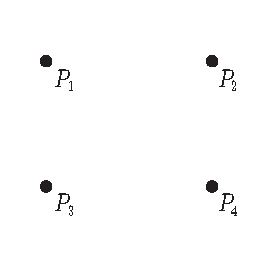
\includegraphics[trim=0cm 0cm 0cm 0cm,clip,scale=0.50]{images/fourpoints1.pdf}
		\item 3 punti allineati su una retta.
		
\includegraphics[trim=0cm 0cm 0cm 0cm,clip,scale=0.50]{images/fourpoints2.pdf}
		\item 4 punti allineati su una retta.
		
\includegraphics[trim=0cm 0cm 0cm 0cm,clip,scale=0.50]{images/fourpoints3.pdf}
	\end{itemize}
	Se i punti $P_i$ sono proiettivamente equivalenti ai punti $Q_i$, allora tali posizioni \textit{devono essere mantenute}: le proiettività mandano \textit{rette in rette}, \textit{posizioni generali in posizioni generali}. Per contronominale, se si verificano casi diversi per le due quaterne possiamo affermare che \textit{non} sono proiettivamente equivalenti.
	\begin{enumerate}
		\item Sia $P_i$, sia $Q_i$ sono in \textit{posizione generale}. Siccome abbiamo 4 punti e $4=\dim\proj[2]{\kamp}+2$, allora $\exists !$ proiettività $f$ di $\proj[2]{\kamp}$ tale che $f(P_1)=Q_i, i=1,\ \ldots,\ 4$, dunque hanno lo stesso \textit{birapporto} e sono sempre \textit{proiettivamente equivalenti}.
		\item $P_1,\ P_2,\ P_3$ \textbf{allineati ma non} $P_4$, \textbf{e lo stesso per i} $Q_i$; in altre parole, $P_1,\ P_2,\ P_3\in r$ retta proiettiva e $Q_1,\ Q_2,\ Q_3\in s$ retta proiettiva.
		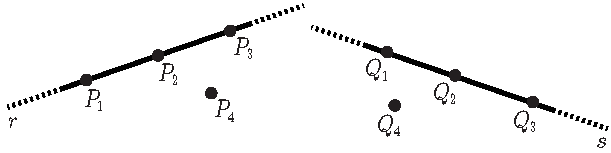
\includegraphics[trim=0cm 0cm 0cm 0cm,clip,scale=0.50]{images/fourpointseq1.pdf}
		Vogliamo dimostrare che anche in questo caso le quaterne sono proiettivamente equivalenti,
%sfruttando la proiettività fra i tre punti ed estendendola al quarto punto
		Scegliamo dei rappresentanti $P_i=[v_i],\ i=1,\ 2,\ 3,\ 4, v_i\in\kamp^3$ tale che $v_3=v_1+v_2$, lecito in quando i punti non sono allineati. Si ha che $\{v_1,\ v_2,\ v_4\}$ è una base di $\kamp^3$: $P_4\notin r$ significa che $v_4$ non è linearmente dipendente da $v_1,\ v_2$. Allo stesso modo sia $Q_i=[w_i],\ i=1,\ 2,\ 3,\ 4, w_i\in\kamp^3$ tale che $w_3=w_1+w_2$ con $\{w_1,\ w_2,\ w_4\}$ base di $\kamp^3$. \\
		Definiamo $\funz \phi {\kamp^3} {\kamp^3}$ lineare tale che:
		\begin{equation*}
			\phi(v_1)=w_1, \phi(v_2)=w_2, \phi(v_4)=w_4
		\end{equation*}
		In questo modo $\phi(v_3)=\phi(v_1+v_2)=w_1+w_2=w_3$. Dunque $\funz {f=\widetilde{\phi}} {\proj[2]{\kamp}} {\proj[2]{\kamp}}$ è una proiettività che manda $P_i$ in $Q_i,\ \forall i=1,\ 2,\ 3,\ 4$.
		\item \textbf{Tutti i punti sono allineati}.
		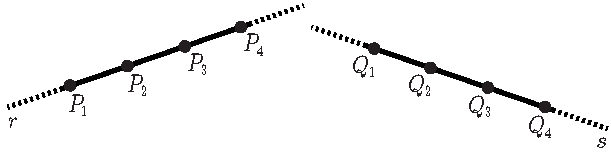
\includegraphics[trim=0cm 0cm 0cm 0cm,clip,scale=0.50]{images/fourpointseq2.pdf}
		Essendo allineati, allora è definito il loro birapporto. Se le due quaterne sono proiettivamente equivalenti, sia $\funz f {\proj[2]{\kamp}} {\proj[2]{\kamp}}$ la proiettività: essa porta una quaterna nell'altra e necessariamente una retta nell'altra, ovvero $f(r)=s$; in altre parole, la restrizione alle due rette $\funz {f_{|_r}} r s$ porta $P_i$ in $Q_i,\ \forall i \implies \beta(P_i)=\beta(Q_i)$.\\
		Viceversa, se $\beta(P_i)=\beta(Q_i)$ allora $\exists \funz g r s$ trasformazione proiettiva che manda $P_i$ in $Q_i,\ \forall i=1,\ 2,\ 3,\ 4$.\\
		Si ha che $g$ si estende in maniera non unica ad una proiettività di $\proj[2]{\kamp}$. Infatti dati:
		\begin{itemize}
			\item $r=\proj{U},\ U\subset \kamp^3$.
			\item $s=\proj{W},\ W\subset\kamp^3$.
		\end{itemize}
		Con $U$ e $W$ piani vettoriali, si ha che $g=\widetilde{\psi}$ con $\funz \psi U W$ è un isomorfismo lineare. Vogliamo estenderla ad un \textit{automorfismo lineare} $\funz \phi {\kamp^3} {\kamp^3}$ scegliendo basi con due vettori nel piano ed uno esterno, ovvero $u_1,\ u_2\in U$ base di $U$ e $u_3\notin U$. Dunque $\{\psi(u_1),\psi(u_2)\}$ è una base di $W$ e $w_3\notin W \implies \{u_1,u_2,u_3\}$ base di $\kamp^3$ e $\{\psi(u_1),\psi(u_2),\psi(u_3)\}$ un'altra base. Ponendo $\funz \phi {\kamp^3} {\kamp^3}$ tale che:
		\begin{itemize}
			\item $\phi(u_1)\coloneqq \psi(u_1)$.
			\item $\phi(u_2)\coloneqq \psi(u_2)$.
			\item $\phi(u_3)\coloneqq w_3$
		\end{itemize}
		Si ha $f=\widetilde{\phi}$. Dunque, i punti sono \textit{proiettivamente equivalenti} se e solo se hanno lo \textit{stesso birapporto}.
	\end{enumerate} 
\end{example}
\subsection{Eserciziamoci! Birapporto}
\begin{exercise}
	Verificare che se $P_1,\ P_2,\ P_3,\ P_4$ sono tutti diversi da $(1\colon 0)$, cioè $P_i=(w_i\colon 1),\ \forall i=1,\ \ldots,\ 4$ e:
	\begin{equation}
		\beta=\frac{ (w_2-w_1)(w_3-w_2) }{ (w_4-w_2)(w_3-w_1) }
	\end{equation}
\end{exercise}
%STUDIO DELLA GEOMETRIA DI RETTE O CURVE NEL PIANO PROIETTIVO
		\section{Piano proiettivo duale}
Una \textbf{retta} in $\proj[2]{\kamp}$ ha equazione:
\begin{equation}
	r\ \colon a_0x_0+a_1x_1+a_2x_2=0
\end{equation}
Essa è un'\textbf{equazione lineare omogenea} in coordinate omogenee, dunque è determinata dai coefficienti $a_0,\ a_1,\ a_2$ dell'equazione con la proprietà che devono essere \textit{non tutti nulli}; inoltre, fissati i coefficienti, l'equazione è determinata \textit{a meno di costante moltiplicativa non nulla}. Dunque si può associare a $r$ un \textbf{punto} del piano proiettivo dato dai coefficienti delle coordinate omogenee:
\begin{equation}
	(a_0\colon a_1\colon a_2)\in\proj[2]{\kamp}
\end{equation}
Si ha una \textit{corrispondenza biunivoca} fra le rette in $\proj[2]{\kamp}$ e $\proj[2]{\kamp}$:
	% https://q.uiver.app/?q=WzAsNCxbMCwwLCJcXHtcXHRleHR7cmV0dGUgaW4gfSBcXHByb2pbMl17XFxrYW1wfVxcfSJdLFszLDAsIlxccHJvalsyXXtcXGthbXB9Il0sWzAsMSwiclxcY29sb24gYV8weF8wK2FfMXhfMSthXzJ4XzI9MCJdLFszLDEsIihhXzBcXGNvbG9uIGFfMVxcY29sb24gYV8yKSJdLFswLDEsIiIsMCx7InN0eWxlIjp7InRhaWwiOnsibmFtZSI6ImFycm93aGVhZCJ9fX1dLFsyLDMsIiIsMCx7InN0eWxlIjp7InRhaWwiOnsibmFtZSI6ImFycm93aGVhZCJ9fX1dXQ==
	\[\begin{tikzcd}
		{\{\text{rette in } \proj[2]{\kamp}\}} &&& {\proj[2]{\kamp}} \\[-25pt]
		{r\colon a_0x_0+a_1x_1+a_2x_2=0} &&& {(a_0\colon a_1\colon a_2)}
		\arrow[from=1-1, to=1-4, tail reversed]
		\arrow[from=2-1, to=2-4, tail reversed]
	\end{tikzcd}\]
% Notiamo che ciò funziona bene con $\proj[2]{\kamp}$, infatti le coordinate omogenee si comportano proprio come i coefficienti dell'equazione.
\begin{example}
In $\proj[2]{\realset}$:
		\begin{equation*}
			l_i\colon x_0+x_1+2x_2=0 \longleftrightarrow (1\colon 1\colon 2)\in\proj[2]{\realset}
		\end{equation*}
	\vspace{-6mm}
\end{example}
\begin{define}\textsc{Piano proiettivo duale.}\\
	Inteso $\proj[2]{\kamp}$ come lo spazio che \textit{parametrizza le rette} in $\proj[2]{\kamp}$, lo chiamiamo \textbf{piano proiettivo duale} \index{piano!proiettivo!duale} e lo denotiamo con $\proj[2]{\kamp}^{\ast}$.
\end{define}
In prima istanza, questo significa semplicemente che si interpreta un punto del \textit{piano duale} come un punto \textit{associato} ad una \textit{retta} di $\proj[2]{\kamp}$.
%collgamento co lo spazio vettoriale duale forma lineare, prima costruzione come corrispondenza
\subsection{Fascio di rette}
\begin{define}\textsc{Fascio di rette}.\\
	Un \textbf{fascio di rette}\index{fascio!di rette} $\mathcal{F}$ in $\proj[2]{\kamp}$ è l'insieme delle rette di equazione:
		\begin{equation}
			\mathcal{F}\colon \lambda l_1+\mu l_2=0, \ (\lambda\colon\mu)\in\proj[1]{\kamp}
		\end{equation}
	Dove $l_1,\ l_2$ sono due rette fissate e distinte.
\end{define}
\begin{observe}
	Possiamo pensare al fascio di rette come una \textbf{collezione di rette}, le cui equazioni si ottengono come \textit{combinazione lineare} delle due rette del fascio con $\lambda,\ \mu$ come \textbf{parametri}.
\end{observe}
\begin{example}
	Consideriamo le rette $l_1\colon x_0+x_1+2x_2=0$ e $l_2\colon 3x_0-2x_1+4x_2=0$. Il fascio di rette determinato da $l_1,\ l_2$ è
		\begin{gather*}
			(\lambda+3\mu)x_0+(\lambda-2\mu)x_1+2(\lambda+2\mu)x_2=0	
		\end{gather*}
	\begin{itemize}
		\item $(\lambda\colon\mu)=(1\colon 0) \rightarrow l_1$.
		\item $(\lambda\colon\mu)=(0\colon 1) \rightarrow l_2$.
		\item $(\lambda\colon\mu)=(1\colon 1) \colon 4x_0-x_1+6x_2=0$.	
	\end{itemize}
\vspace{-3mm}
\end{example}

\begin{observe}
	Abbiamo detto che ad ogni retta corrisponde un punto del piano proiettivo duale. Il fascio $\mathcal{F}$ corrisponde, sul piano duale $\proj[2]{\kamp}^{\ast}$, alla \textbf{retta} passante per i punti corrispondenti a $l_1$ e $l_2$:
		\begin{gather*}
			l_1\colon a_0x_0+a_1x_1+a_2x_2=0 \longrightarrow (a_0\colon a_1\colon a_2)\\
			l_2\colon b_0x_0+b_1x_1+b_2x_2=0 \longrightarrow (b_0\colon b_1\colon b_2)\\
			\mathcal{F}\colon (\lambda a_0+\mu b_0)x_0+ (\lambda a_1+\mu b_1)x_1 +(\lambda a_2+\mu b_2)x_2=0 \rightarrow (\lambda a_0+\mu b_0 \colon \lambda a_1+\mu b_1 \colon \lambda a_2+\mu b_2)
		\end{gather*}
	In altri termini, $(\lambda a_0+\mu b_0 \colon \lambda a_1+\mu b_1 \colon \lambda a_2+\mu b_2)$ rappresenta la retta per i due punti duali \textit{in forma parametrica}.
\end{observe}
\begin{example}
	Prendiamo:
		\begin{gather*}
			\begin{array}{l}
				l_1 \longleftrightarrow (1\colon 1\colon 2)=Q_1\\
				l_2\colon 3x_0-2x_1+4x_2=0 \longleftrightarrow (3\colon -2\colon 4)=Q_2\\
			\end{array}
			\mathcal{F} \longleftrightarrow (\lambda+3\mu \colon \lambda-2\mu \colon 2(\lambda+2\mu))
		\end{gather*}
	Il fascio rappresenta la retta $\overline{Q_1Q_2}$ in forma \textit{parametrica}.
\end{example}
\begin{observe}
	Siccome due rette distinte nel piano si intersecano \textit{in un punto solo}, consideriamo $P\coloneqq l_1\cap l_2$. Allora:
		\begin{itemize}
			\item Ogni retta del fascio passa per $P$ perché è lì che la combinazione lineare \textit{si annulla}.
			\item $P$ è l'unico punto comune a tutte le rette del fascio $\mathcal{F}$.
			\item Viceversa, ogni retta per $P$ appartiene al fascio $\mathcal{F}$.
		\end{itemize}
	Ciò significa che $\mathcal{F}$ è la \textit{famiglia delle rette} per il punto fissato $P$, che è detto \textbf{punto base del fascio}\index{punto!base di un fascio}. 
	%P PUZZA DI SOTTOSPAZIO VETT CON VETT NULLO P 
\end{observe}
\begin{example}
	Consideriamo:
		\begin{gather*}
			\begin{cases}
				l_1\colon x_0+x_1+2x_2=0\\
				l_2\colon 3x_0-2x_1+4x_2=0
			\end{cases} \implies \begin{cases}
				x_0=-x_1-2x_2\\
				-3x_1-6x_2-2x_1+4x_2=0\implies -5x_1-2x_2=0
			\end{cases}\\
		\implies \begin{cases}
			x_0=4x_1\\
			x_2=-\frac{5}{2}x_1
		\end{cases}
			\end{gather*}
		Otteniamo, a meno di multipli, il punto $P=(8\colon 2\colon -5)=l_1\cap l_2$
	Tale fascio $\mathcal{F}$ corrisponde alla retta in $\left(\proj[2]{\ }\right) ^{\ast}$ per i punti $Q_1=(1\colon 1 \colon 2)$ e \\ $Q_2=(3\colon -2\colon 4)$ che, scritta in forma \textit{parametrica}, corrisponde a $(\lambda+3\mu \colon \lambda-2\mu \colon 2(\lambda+2\mu))$. Cerchiamo ora l'equazione \textit{cartesiana} della retta $\overline{Q_1 Q_2}$ nelle coordinate $(a_0\colon a_1\colon a_2)$:
	\begin{gather*}
	\left| \begin{array}{ccc}
		a_0 & a_1 & a_2\\
		1 & 1 & 2 \\
		3 & -2 & 4 \end{array} \right| = 8a_0 + 2a_1-5a_2=0
	\end{gather*}
	Notiamo che i coefficienti della retta ottenuta sono esattamente le \textbf{coordinate omogenee} di $P$, intersezione delle due rette!
\end{example}
Più in generale, fissato un punto base $P\in\proj[2]{\kamp}$, l'insieme delle rette per $P$ in $\proj[2]{\kamp}$:
\begin{equation}
	\mathcal{F}_P=\{\text{rette per }P\text{ in }\proj[2]{\kamp}\}
\end{equation}
È un fascio di rette corrispondente a una \textbf{retta} nel piano proiettivo duale $\left(\proj[2]{\kamp}\right)^{\ast}$. Se le coordinate del punto sono $P=(c_0\colon c_1\colon c_2)$, la retta corrispondente nel piano proiettivo duale $\left(\proj[2]{\kamp}\right)^{\ast}$ ha equazione cartesiana:
\begin{equation}
	c_0a_0+c_1a_1+c_2a_2=0
\end{equation}
Infatti, data una retta $r$ qualsiasi di equazione $a_0x_0+a_1x_1+a_2x_2=0$, il punto $P$ appartiene a $r$, cioè $P\in r$, se e solo se vale l'equazione precedente $c_0a_0+c_1a_1+c_2a_2=0$.\\
Per scrivere il fascio $\mathcal{F}$ in forma \textit{parametrica} scelgo due rette distinte passanti per $P$.
%    sostituisco le coordinate di P e trovo quell'eq:   condizione perchè appartenga alla retta   o al fascio, collezione delle rette per p     fisso p e retta che varia (duale )   retta r fissata e p che varia. Ma l'eq è la stessa. Di fatto il fascio si scrive in forma parametrica scegliendo due rette specifiche che passano per p
\begin{observe}\textsc{Interpretazione affine del fascio di rette proiettive.}\\
	Se interpretiamo $\aff{\kamp^2}=U_0\subset\proj[2]{\kamp}$ e consideriamo il fascio di rette proiettive $\mathcal{F}$ con punto base $P$ in $\proj[2]{\kamp}$, abbiamo due possibilità: $P$ è punto base \textit{proprio} o \textit{all'infinito}.
	\begin{itemize}
	\item Se $P$ è un \textbf{punto proprio}, allora $P\in\aff{\kamp^2}$ e $\mathcal{F}$ corrisponde al  \textit{rette affini} in $\kamp^2$ per il punto $P$ (passando dalla chiusura proiettiva della retta proiettiva a quella affine).
	\item Se $P$ invece è un \textit{punto improprio}, esso corrisponde ad una \textit{direzione} di rette nel piano affine e $\mathcal{F}$ corrisponde a tutte le rette affini che hanno questa direzione fissata, ovvero è un \textbf{fascio di rette parallele}.
	\end{itemize}
	Il caso proiettivo è interessante perché la distinzione fra questi due tipi di fasci è data solo dal fatto se il punto $P$ è proprio o improprio.  	
\end{observe}
\subsection{Spazi vettoriali duali e spazi proiettivi duali}
Sappiamo che $\proj[2]{\kamp}$ è il proiettivizzato di $\kamp^3$, ovvero $\proj[2]{\ }=\proj[2]{\kamp^3}$. Inoltre, in \textit{Geometria Uno}, abbiamo definito gli \textbf{spazi vettoriali duali} come\footnote{A differenza della notazione vista in \textit{Geometria Uno}, qui consideriamo gli indici delle coordinate da $0$ a $2$.}:
\begin{equation}
	\begin{array}{lll}
		\left(\kamp^3\right)^{\ast}&=&\{\text{forme lineari }\alpha\text{ su }\kamp^3\}\\
		& & \funz \alpha {\kamp^3} \kamp\\
		& & \ \, \, \alpha(x_0,\ x_1,\ x_2)= ax_0+a_1x_1+a_2x_2
	\end{array}
\end{equation}
Quando consideriamo la retta $r\colon a_0x_0+a_1x_1+a_2x_2=0$, $r$ è il proiettivizzato del \textbf{nucleo} di $\alpha$, il quale è un \textit{piano vettoriale} $\ker\alpha\subset\kamp^3$ la cui equazione è appunto $a_0x_0+a_1x_1+a_2x_2=0$.\\
In altre parole, si ha una corrispondenza fra i \textit{punti della retta proiettiva duale} e le \textit{classi proiettive} delle forme lineari $[\alpha]$:
\begin{equation}
	\begin{array}{ccc}
		\left( \proj[2]{\ }\right)^{\ast}&=&\proj[2]{\kamp^3}^{\ast}\\ 
		r & \longleftrightarrow & [\alpha]\\
	\end{array}
\end{equation}
Infatti, $\alpha$ è una forma lineare \textit{non nulla} determinata \textit{a meno di multipli}. Si ha che $\{x_0,\ x_1,\ x_2\}$ è una base di $(\kamp^3)^{\ast}$ che induce le coordinate proiettive $(a_0\colon a_1\colon a_2)$ su $\left( \proj[2]{\ }\right)^{\ast}$.\\
Pertanto, tale \textit{interpretazione astratta} diventa operativa fissando la \textit{base duale} delle forme lineari: scrivo $\alpha$ come combinazione lineare della base, e i coefficienti saranno le  data dalle \textit{coordinate proiettive associate}.
Generalizziamo ulteriormente ad uno spazio vettoriale qualunque.
\begin{define}\textsc{Spazio proiettivo duale}.\\
	Dato uno spazio vettoriale $V$, il suo \textit{spazio proiettivo associato} $\proj{V}$ ed il suo \textit{spazio vettoriale duale} $V^{\ast}=\{\text{forme lineari }\funz \alpha V \kamp \}$, si definisce lo \textbf{spazio proiettivo duale}\index{spazio!proiettivo!duale} di $\proj[n]{V}$:
	\begin{equation}
		\proj{V}^{\ast}=\proj{V^{\ast}}
	\end{equation}
	Poichè $\dim V^{\ast} = \dim V$, allora $\proj{V}^{\ast} =\proj{V}$.
\end{define}
In particolare, si ha la corrispondenza biunivoca:
% https://q.uiver.app/?q=WzAsNCxbMCwwLCJcXHByb2p7Vn1ee1xcYXN0fSJdLFszLDAsIlxce1xcdGV4dHtpcGVycGlhbmkgZGkgfSBcXHByb2p7Vn0gXFx9Il0sWzAsMSwiW1xcYWxwaGFdIl0sWzMsMSwiXFxwcm9qe1xca2VyXFxhbHBoYX1cXHN1YnNldFxcbWF0aGJie1B9KFYpIl0sWzAsMSwiIiwwLHsic3R5bGUiOnsidGFpbCI6eyJuYW1lIjoiYXJyb3doZWFkIn19fV0sWzIsMywiIiwwLHsic3R5bGUiOnsidGFpbCI6eyJuYW1lIjoiYXJyb3doZWFkIn19fV1d
\[\begin{tikzcd}
	{\proj{V}^{\ast}} &&& {\{\text{iperpiani di } \proj{V} \}} \\
	{[\alpha]} &&& {\mathbb{P}\left(\ker \alpha\right)\subset\proj{V}}
	\arrow[from=1-1, to=1-4, tail reversed]
	\arrow[from=2-1, to=2-4, tail reversed]
\end{tikzcd}\]
In coordinate, ad un piano di equazione $a_0x_0+\ldots +a_nx_n=0$ associamo il punto $(a_0\colon\ldots\colon a_n)$, nello stesso modo in cui ad un vettore associo i coefficienti della scrittura secondo una tale base.
\subsection{Impratichiamoci! Piano proiettivo duale}
\begin{exercise}
	In $\proj[2]{\realset}$ scrivere in forma parametrica il fascio delle rette per il punto base $P$ di coordinate $(1\colon -1 \colon 4)$.
\end{exercise}
\begin{solution}
	Scegliamo 2 rette distinte, a nostro piacere, che passano per il punto $P$; ad esempio, $l_1\colon x_0+x_1=0$ e $l_2\colon 4x_0-x_2=0$. Il fascio sarà: 
	\begin{gather*}
		\begin{array}{cc}
			\mathcal{F}\colon \lambda(x_0+x_1)+\mu(4x_0-x_2)=0 &  \\
			(\lambda+4\mu)x_0+\lambda x_1-\mu x_2=0,\ & (\lambda\colon\mu)\in\proj[1]{\ }
		\end{array}
	\end{gather*}
	Se facciamo variare $\lambda$ e $\mu$ otteniamo tutte le rette di $\proj[2]{\realset}$ che passano per $P$.
\end{solution}
% io separerei le coniche in un capitolo nuovo, che ne pensi?
\section{Coniche nel piano proiettivo}
Durante \textit{Geometria 1} abbiamo analizzato le coniche nel piano affine $\mathcal{A}(\realset^2)$ e le abbiamo classificate \textit{a meno di rototraslazione}. Vogliamo trattare ora dell'estensione al \textit{piano proiettivo} di queste coniche, tenendo dunque conto del ruolo svolto dalla \textit{retta all'infinito}.\\
Consideriamo $\proj[2]{\kamp}$ con coordinate omogenee $(x_0\colon x_1\colon x_2)$. Indichiamo con $\kamp\left[x_0,\ x_1,\ x_2\right]$ l'\textit{anello dei polinomi} in $x_0,\ x_1,\ x_2$ a coefficienti in $\kamp$. Se $F\in\kamp\left[x_0,\ x_1,\ x_2\right]$ è un polinomio \textit{qualsiasi}, l'equazione $F(x_0,\ x_1,\ x_2)=0$ \textit{non} dà una condizione \textit{ben definita} in $\proj[2]{\kamp}$: ad esempio, $x_0+1=0$ non ha senso perché $x_0$ è determinato solo a meno di multipli. Cerchiamo dunque dei polinomi che ha senso studiare in $\proj[2]{\kamp}$.
\begin{define}\textsc{Polinomio omogeneo}.\\
Sia $F\in\kamp\left[x_0,\ x_1,\ x_2\right]$ un polinomio. Si dice che $F$ è un \textbf{polinomio omogeneo}\index{polinomio!omogeneo} se tutti i monomi a coefficienti \textit{non} nulli hanno lo \textit{stesso} grado.
\end{define}
% Notiamo che la definizione è significativa per polinomi a più variabili, altrimenti i polinomi omogenei sarebbero solo monomi. (non ho questa nota :/)
\begin{examples}~{}
	\begin{itemize}
		\item $F=x_0^3+x_0x_1^2-3x_1x_2x_3\in\realset\left[x_0,\ x_1,\ x_2\right]$ è un polinomio omogeneo di grado $3$.
		\item $G=x_0^3-x_1x_2+1$ non è un polinomio omogeneo.
	\end{itemize}
\vspace{-3mm}
\end{examples}

\begin{observe}
Se $\deg F=1$, cioè $F=a_0x_0+\ldots+a_nx_n+b$, allora $F$ è omogeneo se e solo se $b=0$.
\end{observe}

\begin{observe}
Se $F\in\kamp\left[x_0,\ x_1,\ x_2\right]$ è omogeneo di grado $d$ allora:
\begin{equation}
F(\lambda x_0,\ \lambda x_1,\ \ldots,\ \lambda x_n)=\lambda^d F(x_0,\ \ldots,\ x_n)
\end{equation}
Infatti, $F$ è somma di monomi di grado $d$ del tipo $ax_0^{i_0}x_1^{i_1}\cdots x_n^{i_n}$ con $\displaystyle\sum_{j=0}^n i_j=d$ e si ha che $a(\lambda x_0)^{i_0} (\lambda x_1)^{i_1} \cdots (\lambda x_n)^{i_n}=\lambda^{i_0+\ldots +i_n} (ax_0^{i_0}\ldots x_n^{i_n})=\lambda^d(ax_0^{i_0}\ldots x_n^{i_n})$.
\end{observe}
Torniamo al piano proiettivo $\proj[2]{\ }$ con le coordinate omogenee $(x_0\colon x_1\colon x_2)$ e consideriamo $F\in\kamp\left[x_0,\ x_1,\ x_2\right]$ un polinomio omogeneo nelle coordinate omogenee di grado $d$. Se abbiamo un punto $P=(c_0\colon c_1\colon c_2)\in\proj[2]{\ }$, allora tutte le possibili scelte per le coordinate di $P$ sono $(\lambda c_0\colon \lambda c_1 \colon \lambda c_2)$ con $\lambda\in\kamp\setminus\{0\}$. Valutando $F$ in $P$, otteniamo $F(\lambda c_0,\ \lambda c_1,\ \lambda c_2)=\lambda^d F(c_0,\ c_1,\ c_2)$: in altre parole, $F$ si annulla in una scelta di coordinate se e solo se si annulla in qualsiasi scelta di coordinate, cioè: 
\begin{equation*}
F(c_0,\ c_1,\ c_2)=0\iff F(\lambda c_0,\ \lambda c_1,\ \lambda c_2)=0,\ \forall \lambda\in\kamp\setminus\{0\}
\end{equation*}
Pertanto, l'equazione $F(x_0,\ x_1,\ x_2)=0$ è ben posta in $\proj[2]{\ }$.
\begin{example}
$x_0^2-x_1x_2=0$ definisce un sottoinsieme del piano proiettivo.
\end{example}
\begin{define}\textsc{Curva algebrica piana proiettiva}.\\
	Una \textbf{curva algebrica piana proiettiva}\index{curva!algebrica!proiettiva} $C$ di $\proj[2]{\ }$ è il luoghi degli zeri dato da un polinomio omogeneo $F\in\kamp\left[x_0,\ x_1,\ x_2\right]$:
	\begin{equation}
		C=\left\{(x_0,\ x_1,\ x_2)\in\proj[2]{\ }\mid F(x_0,\ x_1,\ x_2)=0\right\}
	\end{equation}
	La curva è definita a meno di multipli: se $G=\lambda F$ con $\lambda\in\kamp\setminus\left\{0\right\}$, $G$ e $F$ descrivono la stessa curva.\\
	Diciamo che la curva $C$ è \textbf{reale} se $\kamp=\realset$ (e quindi $C\in\proj[2]{\realset}$), \textbf{complessa} se $\kamp=\complexset$ (e quindi $C\in\proj[2]{\complexset}$).
\end{define}
\begin{define}\textsc{Equazione di una curva}.\\
	L'\textbf{equazione}\index{equazione!di una curva} di una curva $C$ è il polinomio $F$ (a a meno di multipli) che la descrive.
\end{define}
\begin{define}\textsc{Supporto di una curva}.\\
	Il \textbf{supporto}\index{supporto} di una curva $C$ descritta da un polinomio $F$ (a a meno di multipli) è l'insieme dove il polinomio si annulla.\\
	L'equazione determina il supporto, ma in generale non vale il contrario.
\end{define}
\begin{define}\textsc{Grado di una curva}.\\
	Il \textbf{grado}\index{grado!di una curva} della curva $C$ è il grado dell'equazione $F$.
\end{define}
\begin{example}
	Preso il polinomio $F(x_0,\ x_1,\ x_2)=a_0x_0+a_1x_1+a_2x_2=0$,la curva $C$ descrive una retta.
\end{example}
\begin{define}\textsc{Rette e coniche proiettive}.
	\begin{itemize}
		\item Le \textbf{rette proiettive} sono curve di grado $1$.
		\item Le \textbf{coniche proiettiva} sono curve di grado $2$.
	\end{itemize}
\vspace{-3mm}
\end{define}
%LEZ 33
D'ora in poi ci restringeremo ai casi $\kamp=\realset$ e $\kamp=\complexset$.
\begin{define}\textsc{Curva irriducibile}.\\
Una curva $C$ è \textbf{irriducibile}\index{curva!irriducibile} se lo è la sua equazione $F$. Altrimenti si considera la sua fattorizzazione in irriducibili:
\begin{equation}
	F=F_1^{m_1}\cdot \ldots \cdot F_r^{m_r}
\end{equation}
Siccome ogni fattore irriducibile $F_i$ è omogeneo, ognuno definisce una curva $C_i\colon F_i=0$, dette \textbf{componenti irriducibili}\index{componenti irriducibili della curva} della curva $C$.\\
Se $m_i>1$ diciamo che $C_i$ è una componente di \textbf{molteplicità}\index{molteplicità} $m_i$ in $C$
\end{define}

\begin{examples}
	\begin{itemize}
		\item Le rette, essendo curve di grado 1, sono \textit{sempre} \textbf{irriducibili}.\\
		Le coniche sono curve di grado 2. Dunque, considerata una conica $C$ di equazione $F=0$, ci sono 3 possibilità:
		\begin{enumerate}
			\item	$C$ è \textbf{irriducibile}.
			\item	$C$ è il prodotto di fattori lineari distinti e non multipli:
			\begin{equation}
				F=L_1\cdot L_2
			\end{equation}
			Con $L_i$ forme lineari \textit{non} proporzionali. Pertanto, $C$ è una \textbf{coppia di rette distinte} (ad es. $C\colon F=x_0x_1\implies C$ unione delle rette $x_0=0$ e $x_1=0$).
			\item	$C$ è data da fattori lineari associati, cioè $F$ è un quadrato a meno di uno scalare:
			\begin{equation}
				F=\lambda L^2,\ \lambda\in\kamp\setminus\{0\}
			\end{equation}
			Allora $C$ è una \textbf{retta doppia}: la retta è la sola componente irriducibile ed è di molteplicità 2 (ad es. $C\colon F=x_0^2$).
		\end{enumerate}
	\end{itemize}
\vspace{-3mm}
\end{examples}

\subsection{Coniche proiettive}
\begin{define}\textsc{Conica}.\\
		Una \textbf{conica}\index{conica} $C$ di $\proj[2]{\ }$ è il luoghi degli zeri dato da un polinomio omogeneo $F\in\kamp\left[x_0,\ x_1,\ x_2\right]$ di grado 2 in $x_0,\ x_1,\ x_2$ a coefficienti \textit{reali} o \textit{complessi}.
		\begin{equation*}
			F=a_{00}x_0^2 +a_{01}x_0x_1+a_{02}x_0x_2+a_{11}x_1^2+a_{12}x_1x_2+a_{22}x_2^2
		\end{equation*}
\end{define}
In generale, i polinomi omogenei di grado 2 sono \textit{forme quadratiche}. Pertanto, vogliamo associare alla forma la  corrispondente matrice simmetrica.
%forma <---> polinomio omogeneo
Per evitare di dividere per 2 i termini misti, ci è lecito immaginarli già nella forma $2a_{01},\ 2a_{02},\ 2a_{12}$, ottenendo così:
\begin{equation*}
F=a_{00}x_0^2 +2a_{01}x_0x_1+2a_{02}x_0x_2+a_{11}x_1^2+2a_{12}x_1x_2+a_{22}x_2^2
\end{equation*}
Allora la matrice simmetrica $3\times 3$ associata alla forma quadratica è:
\begin{equation}
	A=(a_{ij})=\left(\begin{array}{ccc}
		a_{00} & a_{01} & a_{02}\\
		a_{01} & a_{11} & a_{12}\\
		a_{02} & a_{11} & a_{22}\\
	\end{array}\right)\in S\left(\kamp^{3,3}\right)
\end{equation}
Ed è tale per cui $\displaystyle F=x^tAx$ con $x=\left( \begin{array}{c}
x_0 \\ x_1 \\ x_2
\end{array} \right)$ il vettore delle coordinate omogenee.\\
\begin{define}\textsc{Rango della conica}.\\
Il \textbf{rango}\index{rango!di una conica} della conica $C$ è il rango della matrice associata $A$.
\end{define}
\begin{observe}
Come già osservato, l'equazione della conica $C$ determina $F$ solo a meno di multipli, dunque anche la matrice $A$ è determinata \textit{a meno di multipli}. 
Tuttavia, il rango rimane ben definito in quanto $\rk(\lambda A)=\rk(A),\ \forall\lambda\neq 0$. Inoltre, il rango \textit{non} può essere $0$ perché essendo l'equazione di una conica il polinomio \textit{non} può essere nullo (non descriveremmo una conica!).
\end{observe}
Vogliamo studiare le coniche e le curve di grado maggiore a meno di equivalenza proiettiva, allo stesso modo in cui abbiamo classificato le coniche in $\realset^2$ a meno di rototraslazioni.\\
Sia dunque $\funz f {\proj[2]{\ }} {\proj[2]{\ }}$ una proiettività, la cui matrice associata $M\in\gl(3,\kamp)$ è tale per cui $x'=Mx$. Allora $f$ porta la conica $C\colon F=0$ nella conica $\widetilde{C}\colon \widetilde{F}=0$, dove $\widetilde{F}$ si ottiene sostituendo in $f$ il vettore $x=M^{-1}x'$.
\begin{example}
Sia $C \colon x_ox_1=0$ una coppia di rette e $f$ una proiettività tale che:
\begin{equation*}
	f(x_0\colon x_1\colon x_2)=(x_0+x_1\colon x_0-2x_1\colon x_2)
\end{equation*}
Scriviamo, usando la matrice associata alla proiettività, il vettore immagine $x'_i$ in funzione di $x_i$ e poi ricaviamo $x_i$ in funzione di $x'_i$.
\begin{gather*}
f\colon \begin{cases} 
x'_0=x_0+x_1\\
x'_1=x_0-2x_2\\
x'_2=x_2
\end{cases} \implies \begin{cases}
-3x_1=x'_1-x'_0 \implies x_1=\frac{1}{3}(x'_0-x'_1)\\
x_0=x'_0-x_1=x'_0 -\frac{1}{3}(x'_0-x'_1)=\frac{1}{3}(2x'_0+x'_1)
\end{cases}\\
f^{-1}\colon \begin{cases}
x_0=\frac{1}{3}(2x'_0+x'_1)\\
x_1=\frac{1}{3}(x'_0-x'_1)\\
x_2=x'_2
\end{cases}
\end{gather*}
In sostanza abbiamo ottenuto l'espressione dell'inversa di $f$; quindi, la trasformata di $C$ tramite $f$ è $(2x_01+)(x'_0-x'_1)=0$, che è ancora una coppia di rette. In particolare, notiamo che esse sono le immagini tramite $f$ delle rette $x_0=$ e $x_1=0$, a meno dei fattori moltiplicativi $\frac{1}{3}$.
\end{example}
Osserviamo che la proiettività manda il supporto della prima conica nel supporto della seconda conica e che, trasformando la conica tramite una proiettività, trasformiamo la forma quadratica $F$ tramite un cambiamento di coordinate di $\kamp^3$.\\
Dunque, se $A$ è la matrice associata a $C$ e $\widetilde{A}$ è la matrice associata alla trasformata $\widetilde{C}$ tramite $f$, allora $A$ e $\widetilde{A}$ sono \textbf{congruenti}.
Infatti, il \textit{cambiamento di coordinate} su uno spazio vettoriale per la forma quadratica è dato da $\widetilde{A}=M^tAM$ con $M\in\gl\left(3,\kamp\right)$ con $M$ una matrice associata della proiettività, interpretata come matrice del cambiamento di base.\\
Viceversa, date due coniche $C_1$ e $C_2$ le cui matrici associate (simmetriche) $A_1$ e $A_2$ sono congruenti, allora $C_1$ e $C_2$ sono \textit{proiettivamente equivalenti}:  questo perché, in generale, forme quadratiche congruenti differiscono per un cambiamento di base.\\ Otteniamo così la seguente corrispondenza:
\begin{equation*}
\begin{array}{ccc}
C_1\text{ e }C_2\text{ equivalenti}& \iff & A_1\text{ e }A_2\text{ congruenti}
\end{array}
\end{equation*}
Pertanto lo studio delle coniche, a meno di equivalenze proiettive, passa per lo studio delle matrici congruenti.
\subsection{Classificazione delle coniche proiettive complesse}
\begin{remember}
Nel campo dei complessi ($\kamp=\complexset$) due matrici simmetriche \textit{sono congruenti} se e solo se hanno lo \textit{stesso rango}.
\begin{equation*}
	\begin{array}{ccc}
		A_1\text{ e }A_2\text{ congruenti}& \iff & \rk A_1=\rk A_2
	\end{array}
\end{equation*}
In generale, vale solo che se le matrici simmetriche sono congruenti allora hanno lo stesso rango (ma non il viceversa!).
\end{remember}
Allora, a meno di equivalenza proiettiva, ci sono solo 3 possibili coniche: quelle di rango 1, rango 2 e rango 3.
\begin{theorema}\textsc{Classificazione delle coniche proiettive complesse}.
\begin{enumerate}
\item	Due coniche in $\proj[2]{\complexset}$ sono proiettivamente equivalenti se e solo se hanno lo stesso rango.
\item	\textbf{Forma canonica}: ogni conica di $\proj[2]{\complexset}$ è proiettivamente equivalente ad \textit{una ed una sola} delle tre coniche seguenti:\\
\begin{equation*}
		\begin{array}{cll}
		\underline{\rk 3}\colon & x_0^2+x_1^2+x_3^2=0 &	\text{Conica irriducibile}\\[1mm]
		\underline{\rk 2} \colon & x_0^2+x_1^2=(x_0+ix_i)(x_0-ix_1)=0 & \text{Coppia di rette distinte}\\[1mm]
		\underline{\rk 1} \colon & x_0^2=0 & \text{Retta doppia}
	\end{array}
\end{equation*}
\end{enumerate}
\vspace{-3mm}
\end{theorema}

%questo è dato dalla classificazione delle forme quadratiche du \complexset^3

v\subsection{Classificazione delle coniche proiettive reali}
Sia $C$ una conica in $\proj[2]{\realset}$ con matrice associata $A$, simmetrica \textit{reale} $3\times 3$. Come abbiamo detto, poiché la matrice non è complessa, non è sufficiente il rango per la congruenza: affinché sia congruente ad un'altra matrice simmetrica serve anche la \textbf{segnatura}.
\begin{observe}
Siccome $A$ è determinata a meno di multipli, in principio la segnatura potrebbe cambiare. Vediamo cosa succede effettivamente.\\
Se $A$ ha segnatura $(p,q)$ con $p$ il numero di autovalori \textit{positivi} e $q$ il numero di autovalori \textit{negativi}, allora $\lambda A$ può avere segnatura $(p,q)$ se $\lambda>0$ oppure $(q,p)$ se $\lambda <0$.\\
Quindi, la segnatura di una conica è definita solo ‘‘a meno del segno'', nel senso che $(p,q)=(q,p)$.
\end{observe}
	\begin{theorema}\textsc{Classificazione delle coniche proiettive reali}.
	\begin{enumerate}
	\item	 Due coniche in $\proj[2]{\realset}$ sono proiettivamente equivalenti se e solo se hanno la stessa \textit{segnatura} a meno del segno; dalla segnatura si deduce anche il \textit{rango}.
	\item	Ogni conica in $\proj[2]{\realset}$ è proiettivamente equivalente a una ed una sola delle seguenti coniche, con segnature distinte a meno del segno:
	\begin{equation*}
		\arraycolsep=2.5pt
		\begin{array}{ccll}
			\underline{\rk 3} & \begin{array}{l}
					(3,0)/(0,3) \\
					\\
					(1,2)/(2,1)
				\end{array} & \begin{array}{l}
				x_0^2+x_1^2+x_2^2=0\\
				\\
				x_0^2+x_1^2-x_2^2=0\\
			\end{array} 
				 & \begin{array}{l}
			\begin{array}{l}
				\text{Conica irriducibile senza} \\
				\text{punti reali (supporto vuoto)}
			\end{array} \\
			\begin{array}{l}
				\text{Conica irriducibile a punti reali,} \\
				\text{contiene infiniti punti in }\proj[2]{\realset}
			\end{array}
		\end{array}\\ \hline %ha un supporto? ci sono dei punti in P2R che hanno questa equazione? no perché escludiamo l'origine	conica irriducibile senza punti reali /tipo ellisse immaginario/ dunque il supporto è vuoto
		\underline{\rk 2} &\begin{array}{c}
		(2,0)/(0,2) \\
		\\
		(1,1)
		\end{array} &\begin{array}{l}
		\\[-1mm]
		x_0^2+x_1^2=0 \\
		\\[-1mm]
		x_0^2-x_1^2=\\[-0.75ex]
		=(x_0-x_1)(x_0+x_1)=0
		\end{array} & \begin{array}{l}
		\begin{array}{l}
		\text{Coppia di rette non reali} \\
		\text{con } 1 \text{ punto reale } (0\colon 0\colon 1)
		\end{array} \\ %	perché si fattorizza ma a coeff complessi. Ha un unico punto reale (0\colon 0\colon 1) intersezione delle due rette complesse coniugate
		\begin{array}{l}
		\text{Conica irriducibile a punti reali,} \\
		\text{coppia di rette reali distinte}
		\end{array}
		\end{array} \\[2mm] \hline %che si fattorizza su R
		\underline{\rk 1} & (1,0) & \begin{array}{l}
			\\[-4mm]
			x_0^2=0
		\end{array} &\ \ \begin{array}{l}
		\text{Retta doppia}
	\end{array}	
\end{array}	
	\end{equation*}
	\end{enumerate}
	\end{theorema}

	\subsection{Curve algebriche piane affini e chiusura proiettiva}
Siccome abbiamo interpretato il piano proiettivo come un'\textit{estensione} di quello affine, possiamo confrontare la classificazione delle curve nel piano proiettivo con la \textit{classificazione nel caso affine}.
\begin{define}\textsc{Curva algebrica piana affine}.\\
	Una \textbf{curva algebrica piana affine}\index{curva!algebrica!affine} $C$ di $\aff{\kamp^2}$ è il luoghi degli zeri dato da un polinomio omogeneo $f\in\kamp\left[x,\ y\right]$:
\begin{equation}
	C=\left\{(x,\ y)\in\proj[2]{\ }\mid f(x,\ y)=0\right\}
\end{equation}
La curva è definita a meno di multipli: se $g=\lambda f$ con $\lambda\in\kamp\setminus\left\{0\right\}$, $g$ e $f$ descrivono la stessa curva.\\
Diciamo che la curva $C$ è \textbf{reale} se $\kamp=\realset$ (e quindi $C\in\aff{\realset^2}$), \textbf{complessa} se $\kamp=\complexset$ (e quindi $C\in\aff{\complexset^2}$).
\end{define}
\begin{define}\textsc{Equazione di una curva}.\\
L'\textbf{equazione}\index{equazione!di una curva} di una curva $C$ è il polinomio $f$ (a a meno di multipli) che la descrive.
\end{define}
\begin{define}\textsc{Supporto di una curva}.\\
Il \textbf{supporto}\index{supporto} di una curva $C$ descritta da un polinomio $f$ (a a meno di multipli) è l'insieme dove il polinomio si annulla.\\
L'equazione determina il supporto, ma in generale non vale il contrario.
\end{define}
\begin{define}\textsc{Grado di una curva}.\\
Il \textbf{grado}\index{grado!di una curva} della curva $C$ è il grado dell'equazione $f$.
\end{define}
\begin{define}\textsc{Curva irriducibile}.\\
	Una curva $C$ è \textbf{irriducibile}\index{curva!irriducibile} se lo è la sua equazione $f$. Altrimenti si considera la sua fattorizzazione in irriducibili:
	\begin{equation}
		f=f_1^{m_1}\cdot \ldots \cdot f_r^{m_r}
	\end{equation}
	Siccome ogni fattore irriducibile $f_i$ è omogeneo, ognuno definisce una curva $C_i\colon f_i=0$, dette \textbf{componenti irriducibili}\index{componenti irriducibili della curva} della curva $C$.\\
	Se $m_i>1$ diciamo che $C_i$ è una componente di \textbf{molteplicità}\index{molteplicità} $m_i$ in $C$
\end{define}
\begin{define}\textsc{Rette e coniche affini}.
	\begin{itemize}
		\item Le \textbf{rette affini} $ax+by+c=0$ sono curve di grado $1$.
		\item Le \textbf{coniche affini} $ax^2+by^2+cxy+dx+ey+f=0$ sono curve di grado $2$.
	\end{itemize}
	\vspace{-3mm}
\end{define}
\subsubsection{Omogeneizzazione di un polinomio}
Vediamo ora qual è il legame fra curve affini e proiettive utilizzando la \textit{chiusura proiettiva}. Ricordiamo che $\kamp^2=U_0\subset \proj[2]{\kamp}$ con $(x,\ y)\in\kamp^2$ che corrispondono a $\displaystyle x=\frac{x_1}{x_0}$ e $\displaystyle y=\frac{x_2}{x_0}$, dato $(x_0\colon x_1\colon x_2)\in\proj[2]{\kamp}$.\\
Sia $C$ una curva affine di equazione $f(x,\ y)=0$. Vogliamo associare a $f$ un polinomio omogeneo nelle coordinate $x_0,\ x_1,\ x_2$ dello stesso grado di $f$.
Consideriamo dunque il polinomio $F\in\kamp\left[x_0,\ x_1,\ x_2\right]$ così definito: se $d=\deg f$, allora:
\begin{equation}
	F\coloneqq x_0^d f\left( \frac{x_1}{x_0}, \frac{x_2}{x_0} \right)
\end{equation}
Esso è a tutti gli effetti un polinomio dello stesso grado di $f$. Infatti, $F$ è un polinomio omogeneo di grado $d$: considerato un monomio in $f$, della forma $ax^iy^j$, allora $i+j$ se ne ottiene uno di grado $d$ in $x_0,\ x_1,\ x_2$:
	\begin{equation*}
		ax^iy^j \Longrightarrow x_0^d a \left( \frac{x_1}{x_0} \right)^i \left( \frac{x_2}{x_0} \right)^j = ax_0^{d-i-j} x_1^i x_2^j
	\end{equation*}
Ripetendo questa procedura per ogni monomio si ottiene un polinomio omogeneo $f$ di grado $d$ come desiderato. Notiamo che, operativamente, l'omogeneizzazione consiste nel cambiare nome alle variabili $x$ e $y$ e moltiplicare per un'opportuna potenza di $x_0$ in modo tale che il monomio sia di grado $d$. 
\begin{example} Vogliamo omogenizzare il polinomio $f=x^3-2xy+3y+1$. Prima di tutto si cambia il nome delle variabili e si ottiene $x_1^3-2x_1x_2+3x_2+1$. Moltiplicando ciascun monomio per l'opportuna potenza di $x_0$, il polinomio omogeneizzato rispetto a $x_0$ sarà $F=x_1^3-2x_0x_1x_2 +3x_0^2x_2+x_0^3$.
\end{example}
\begin{observe}
	Possiamo ‘‘deomogeneizzare'' un polinomio omogeneo $F(x_0,\ x_1,\ x_2)$: ponendo $x_0=1$ si riottiene il polinomio di partenza $f(x_1,\ x_2)$.
\end{observe}
\subsubsection{Chiusura proiettiva}
\begin{define}\textsc{Chiusura proiettiva di una curva affine}.\\
	La curva $\overline{C}$ in $\proj[2]{\kamp}$ definita da $F=0$ si dice \textbf{chiusura proiettiva}\index{chiusura!proiettiva!di una curva} della curva affine $C$ di equazione $f=0$.
\end{define}
Se $P=(1\colon x\colon y)\in U_0$  allora $f(x,\ y)=F(P)$ e in particolare $\overline{C}\cap U_0=C$.
\begin{define}\textsc{Punti impropri di una curva}.\\
	I \textit{punti impropri} o \textit{punti all'infinito} della curva $C$ sono dati dall'intersezione della chiusura proiettiva con la \textit{retta impropria}, ovvero da $\overline{C}\cap\{x_0=0\}$
\end{define}
\begin{example}\textsc{Chiusura proiettiva di una retta}.\\
	Se $C$ è una retta $ax+by+c=0$, allora la \textit{chiusura proiettiva} di $C$ è $ax_1+bx_2+cx_0=0$ ed il \textit{punto improprio} di $C$ è $(0\colon -b\colon a)$, che corrisponde alla direzione della retta $C$.
\end{example}

\begin{examples}
	Consideriamo in $\realset^2$ le coniche:
	\begin{equation*}
		\begin{array}{cll}
			C_1\colon & y=x^2 & 	\text{Parabola}\\[1mm]
			C_2\colon & x^2+y^2=1 &		\text{Circonferenza}\\[1mm]
			C_3\colon &	x^2-y^2=1 & \text{Iperbole}
		\end{array}
	\end{equation*}
	Consideriamo ora le loro \textit{chiusure proiettive reali} tramite l'omogeneizzazione, cioè le coniche proiettive $\overline{C_i}$ in $\proj[2]{\realset}$:
		\begin{equation*}
		\begin{array}{cl}
			\overline{C_1} \colon & x_0x_1=x_1^2\\[1mm]
			\overline{C_2} \colon & x_1^2+x_2^2=x_0^2\\[1mm]
			\overline{C_3} \colon & x_1^2-x_2^2=x_0^2
		\end{array}
	\end{equation*}
	Scrivendo le matrici associate e guardandone la segnatura, si vede che \textit{tutte e tre} hanno segnatura $(2,1)/(1,2)$ e quindi tutte proiettivamente equivalenti (per la classificazione delle coniche nel piano proiettivo reale) ad una \textit{conica irriducibile a punti reali} in $\proj[2]{\realset}$.\\
	Consideriamo ora i loro punti impropri:
		\begin{itemize}
			\item \textsc{Parabola}: $\overline{C_1}\cap\{x_0=0\}\colon (0\colon 0\colon 1)$, dunque un solo punto improprio, ovvero la direzione $(0,1)$ dell'asse $y=\mathcal{L}(0,1)$, quindi è l'asse della parabola
			\item \textsc{Circonferenza}: $\overline{C_2}\cap \{x_0=0\} \colon x_0=0 \implies x_1=x_2=0$ ma non si possono avere tute le coordinate omogenee nulle, dunque non ci sono punti impropri 
			\item \textsc{Iperbole}: $\overline{C_3}\cap\{x_0=0\}\colon x_1^2-x_2^2=0$, dunque ci sono	due punti impropri quali $(0\colon 1\colon 1)$ e $(0\colon 1\colon -1)$, a cui corrispondono le direzioni degli asintoti dell'iperbole
		\end{itemize}
	Notiamo che le chiusure proiettive viste sono tutte proiettivamente equivalenti, ma hanno 3 posizioni diverse rispetto alla \textit{retta impropria}:\\
			\begin{minipage}{0.57\textwidth}
			\begin{enumerate}[series=proj2]
				\item $\overline{C_1}$ è ‘‘\textit{tangente}'' alla retta impropria.
			\end{enumerate}
		\end{minipage}
		\begin{minipage}{0.52\textwidth}
					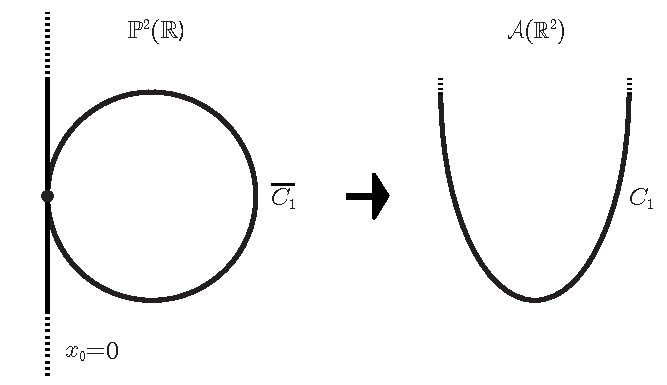
\includegraphics[trim=0cm 0cm 0cm 0cm,clip,scale=0.50]{images/projconic1.pdf}
		\end{minipage}\\
	\begin{minipage}{0.57\textwidth}
		\begin{enumerate}[resume=proj2]
		\item $\overline{C_2}$ è ‘‘\textit{disgiunta}'' dalla retta impropria.
		\end{enumerate}
	\end{minipage}
	\begin{minipage}{0.52\textwidth}
					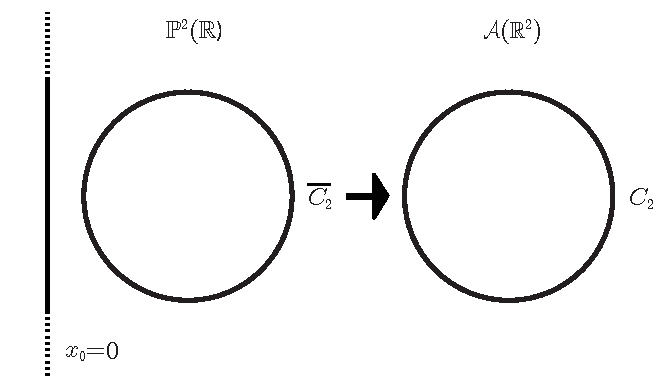
\includegraphics[trim=0cm 0cm 0cm 0cm,clip,scale=0.50]{images/projconic2.pdf}
	\end{minipage}\\
	\begin{minipage}{0.57\textwidth}
	\begin{enumerate}[resume=proj2]
		\item $\overline{C_3}$ è ‘‘\textit{secante}'' rispetto alla retta impropria.
	\end{enumerate}
\end{minipage}
\begin{minipage}{0.52\textwidth}
					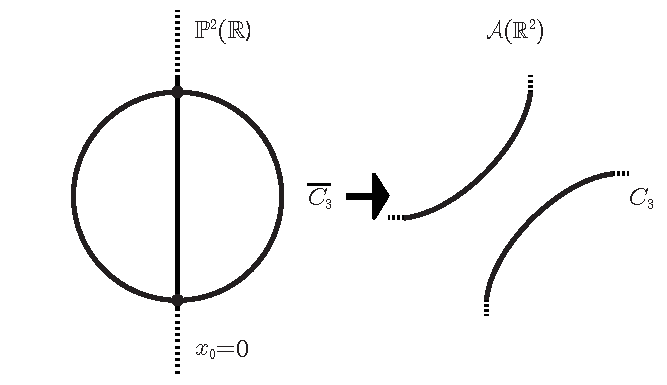
\includegraphics[trim=0cm 0cm 0cm 0cm,clip,scale=0.50]{images/projconic3.pdf}
\end{minipage}
\end{examples}
\begin{example}
	In $\aff{\realset^2}$ consideriamo la coppia di \textit{rette parallele} distinte $x(x+1)=0$ e la coppia di \textit{rette incidenti} distinte $xy=0$.\\
	Prendendo le le chiusure proiettive si ottiene $x_1(x_1+x_0)=0$ e $x_1x_2=0$, entrambe coppie di rette distinte reali in $\proj[2]{\realset}$ con segnatura (1,1). \\
	Dunque sono proiettivamente equivalenti fra loro ma hanno posizione diversa rispetto alla retta impropria.
	\begin{itemize}
		\item La prima ha un solo punto improprio $(0\colon 0\colon 1)$, che è la \textit{direzione comune} delle due rette parallele nel piano affine.
		\begin{center}
			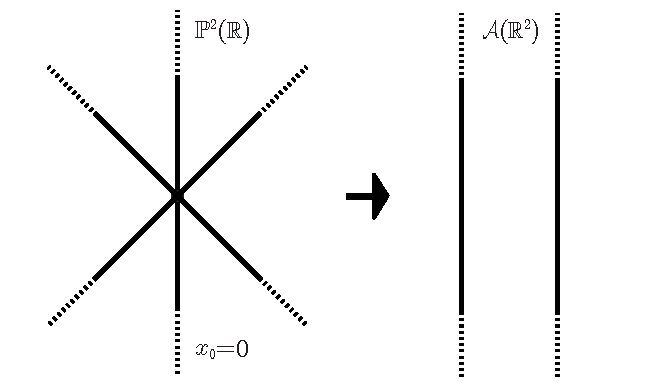
\includegraphics[trim=0cm 0cm 0cm 0cm,clip,scale=0.50]{images/projlineintersect1.pdf}
		\end{center}
		\item La seconda ha due punti impropri $(0\colon 0\colon 1)$ e $(0\colon 1\colon 0)$, che sono le direzioni delle due rette nel piano affine.
		\begin{center}
			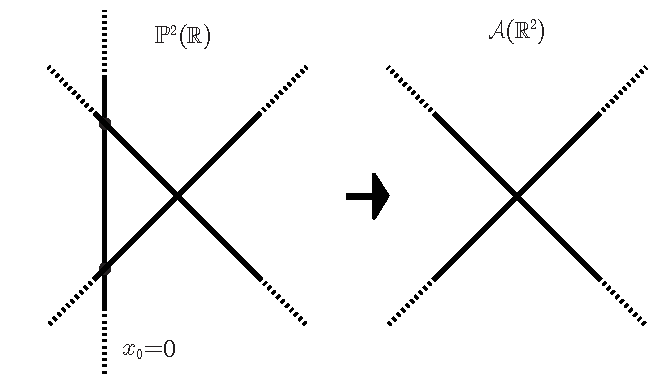
\includegraphics[trim=0cm 0cm 0cm 0cm,clip,scale=0.50]{images/projlineintersect2.pdf}
		\end{center}
	\end{itemize}
\vspace{-3mm}
\end{example}
Ragionando in questo modo dalla classificazione delle coniche proiettive si può mettere in relazione la classificazioni delle coniche affini $\aff{\realset^2}$ (a meno di rototraslazione), prestando attenzione alla posizione rispetto alla retta impropria.
\subsection{Classificazione affine delle coniche nel caso complesso}
\begin{proposition}\textsc{Classificazione delle coniche affini complesse}.
Ogni conica in $\complexset^2$ si può ridurre con una trasformazione del tipo:
\begin{equation}
	\begin{pmatrix} x' \\ y' \end{pmatrix} =A\begin{pmatrix} x \\ y \end{pmatrix} +b
\end{equation}
Con $b\in\complexset^2$ e $A\in\gl(2,\complexset)$ ad una delle cinque coniche:
\begin{center}
	\begin{tabular}{cll}
	1. &	$x^2+y^2+1=0$ & \begin{tabular}{l}
			${\scriptstyle \blacksquare}$ Rango 3.\\
			${\scriptstyle \blacksquare}$ \textit{Due} punti impropri \textit{distinti}.
		\end{tabular}   \\ \hline
	2. &	$y-x^2=0$ & \begin{tabular}{l}
			${\scriptstyle \blacksquare}$ Rango 3.\\
			${\scriptstyle \blacksquare}$ Un \textit{unico} punto improprio.
		\end{tabular}  \\ \hline
	3. &	$x^2+y^2=(x+iy)(x-iy)=0$ & \begin{tabular}{l}
			Coppia di rette distinte \textit{incidenti}:\\
			${\scriptstyle \blacksquare}$ Rango 2.\\
			${\scriptstyle \blacksquare}$ \textit{Due} punti impropri \textit{distinti}.
		\end{tabular} \\ \hline
	4. &	$x(x+1)=0$ & \begin{tabular}{l}
			Coppia di rette distinte \textit{parallele}:\\
			${\scriptstyle \blacksquare}$ Rango 2.\\
			${\scriptstyle \blacksquare}$ Un \textit{unico} punto improprio.
		\end{tabular} \\ \hline
	\begin{tabular}{l}
		\\[-3mm]
		5.
	\end{tabular} &	\begin{tabular}{l}
		\\[-3mm]
		$x^2=0$
	\end{tabular} & \begin{tabular}{l}
		\\[-3mm]
		Retta doppia
	\end{tabular} \\
	\end{tabular}
\end{center}
%	DA RIASCOLTARE
%	vediamo dove andiamo a parare:guardando la chiusura proiettiva, ho 3 ranghi possibili con la loro ir/riducibilità. Dobbamo guarare la posizione possibile rispetto alla retta allìinfinito, Siccome simao su C la chiusura proj ha solo 2 posizioni possibili: 2 punt distini o 2 punti coincidenti se irriducibili in base a 2 pt impropri o un solo. Idem per la coppia di rette al caso 			1 caso in rango 1
\vspace{-3mm}
\end{proposition}
\begin{comment}
	non la dimostriamo ma abbiamo dato una giustificazione geometrica: class a meno di proj e #punti impropri
	RECAP	
	nel piano proj nel piano proj si riduce a classificare le forme quadratiche in K^3 ed usiamo l'algebra lineare: equiv proj dal rango (3 classi) mentr ein quello reale dipende anche dalla segnatura (a meno del segno) ed abbiamo 5 classi di equiv proj di coniche nel pin proj reale
	curve alg aff e chius proj
	class affine coniche in r2 passando alla chiusura proj 
	esempi che spiegao il significato geometrico
	ellisse ierbole etc	chiusura proj stessa ma cambia pos retta impropria
	class affine coniche in c2, guardo anche il numero di punti impropri
	class coniche semplice perché è alg ineare, da grado 3 in su è meno semplice, servono dunque le nozioni per studiare curva algebrica, che sia affine o proiettiva
\end{comment}
	\subsection{Polinomi omogenei in 2 variabili}
I polinomi omogenei in \textit{due variabili} si comportano per alcuni aspetti come polinomi in \textit{una so}la variabile.\\
Sia $F\in\kamp[x_0x_1]$ un polinomio omogeneo di grado $d$, costituito da $d+1$ monomi:
\begin{equation*}
	F=a_0x_0^d+a_1x_0^{d-1}x_1+a_2x_0^{d-2}x_2^2+\ldots + a_{d-1}x_0x_1^{d-1}a_dx_1^d
\end{equation*}
Ricordiamo che vedendo $\left(x_0\colon x_1\right)\in\proj[1]{\ }$, allora $F$ ha degli zeri su $\proj[1]{\ }$, ovvero $F(P)=0$ è ben posto per $P=(a\colon b)\in\proj[1]{\ }$.
\begin{define}\textsc{Annullarsi in un punto}.\\
	Diciamo che $F$ si \textbf{annulla in } $P=(a\colon b)$ \textbf{all'ordine } $m$ se $(ax_1-bx_0)^m$\index{annullarsi in un punto} è la massima potenza di $ax_1-bx_0$ che divide $F$.
\end{define}
%		va letta ome la propr in 1 var come le radici /Ruffini!/
\begin{proposition} \label{teo polinomi omogenei 2 variabili}~{}
	\begin{enumerate}
		\item	$F$ si annulla in un punto $P=(a\colon b)\in\proj[1]{\ } \iff ax_1-bx_0\mid F$.
		\item 	Se $d=\deg F$, $F$ ha al più $d$ zeri su $\proj[1]{\ }$ contati con molteplicità. %/analogo degli zeri 
		\item	Se $F\in\complexset[x_0,\ x_1]$, allora $F$ si fattorizza come prodotto di forme lineari e ha esattamente $d$ zeri in $\proj[1]{\ }$ contati con molteplicità.\footnote{Questo punto è analogo al caso in una variabile per cui, in $\complexset$, ogni polinomio si fattorizza come prodotto di polinomi di grado 1 ed ha tutti gli zeri ben definiti.}.
	\end{enumerate}
\vspace{-3mm}
\end{proposition}
\begin{demonstration}
	% Facciamo un'ipotesi che ci semplificherà la notazione, per poi studiare il caso generale.\\
	Supponiamo che $x_0 \nmid F$; ciò è vero se e solo se $a_d\neq 0$ o, alternativamente, $F(0\colon 1)\neq 0$. Poniamo:
	\begin{equation}
		f\coloneqq F(1,t)\in\kamp[t] = a_0+a_1t+\ldots+a_{d-1}t^{d-1}+a_dt^d
	\end{equation}
	Esso è un polinomio nella sola variabile $t$, dato che abbiamo posto $x_0=1$ e $x_1=t$, ed è ancora di grado $d$ perché $a_d\neq 0\implies \deg f=\deg F=d$. Inoltre:
		\begin{itemize}
			\item $F$ è l'omogeneizzato di $f$ rispetto a $x_0$:
			\begin{equation*}
				F=x_0^2f\left( \frac{x_1}{x_0} \right)
			\end{equation*}
			\item Gli zeri di $F$ sono tutti e soli della forma $(1\colon\lambda)$ con $\lambda$ radice di $f$, dato che \textit{deomogeneizzando} passiamo da 2 variabili in 1 variabile, infatti $F(1,\lambda)=f(\lambda)$.\\
		\end{itemize}
	Pertanto, le proprietà di $F$ che vogliamo dimostrare seguono da quelle di $f$ che conosciamo già.\\
		\begin{enumerate}[label=\Roman*]
			\item $F$ si annulla in $(1\colon\lambda)=(a\colon b) \footnote{Con $\lambda=\frac{b}{a}$.}\iff f(\lambda)=0 \iff t-\lambda \mid f \iff x_1-\lambda x_0\mid F$. %in particolare l'omogeneizzato divide $F$ (non ho questa nota).
			\item È immediato dal punto $1$, perché se $F$ si annulla in $P_i=(a_i\colon b_i)$ distinti con molteplicità $m_i$, allora:
			\begin{equation*}
				(a_ix_1-b_ix_0)^{m_i} \mid F,\ \forall i=1,\ \ldots,\ r 
			\end{equation*}
			Siccome i punti $P_i$ sono distinti, allora i polinomi sono \textit{primi fra loro} al variare di $i$, dunque anche il loro prodotto deve dividere $F$:
			 \begin{equation*}
			 	\prod_{i=1}^r (a_ix_1-b_ix_0)^{m_i}\mid F \implies \sum_{i=1}^r m_i\leq d=\deg F
			 \end{equation*}.
			\item Segue immediatamente dal caso complesso in una variabile; infatti, $f$ si scrive come:
			\begin{equation*}
				f=c(t-\lambda_1)^{m_1}\cdot \ldots\ \cdot (x_1-\lambda_r x_0)^{m_r}
			\end{equation*}
			Siccome $\complexset$ è algebricamente chiuso, $F=c(x_1-\lambda_1x_0)^{m_1}\cdot \ldots\cdot (x_1-\lambda_rx_0)^{m_r}$, cioè si fattorizza completamente con forma lineari. Non solo questo polinomio divide $F$ ma, a meno di costante, ho l'\textit{uguaglianza}, per cui il numero di zeri contati con molteplicità è pari al suo grado.
		\end{enumerate}
	Se invece $x_0\mid F$, allora $F=x_0^r G$ per un certo $r$, con $G$ un polinomio omogeneo di grado $d-r$ tale per cui $x_0\nmid G$. Allora i risultati trovati valgono per $G$ e, tenendo conto che $F$ si annulla in $(0\colon 1)$ con molteplicità $r$, segue la tesi della proposizione.
\end{demonstration}
\subsection{Intersezione tra una retta ed una curva nel piano proiettivo}
%Useremo queste proprietà dei polinomi omogenei di secondo grado per studiare l'intersezione fra una retta ed una curva in $\proj[2]{\ }$.\\
Sia $C$ una curva in $\proj[2]{\ }$ di grado $d$ ed equazione $F(x_0,\ x_1,\ x_2)=0$ e sia $r\subset\proj[2]{\ }$ una retta proiettiva. Vogliamo intersecare la retta $r$ con il supporto di $C$.\\
\begin{tips}
	Per studiare l'intersezione di due sottoinsiemi può essere comodo esprimere uno dei due sottoinsiemi in \textit{forma parametrica} e sostituire i risultati trovati nelle equazioni dell'altro.
\end{tips}
%Di uno ho le equazioni, mentre so come scrivere in forma parametrica la retta
Scriviamo una parametrizzazione per $r$; per farlo sono necessari servono 2 punti distinti $A,B\in r$. In questo modo, ogni punto di $r$ si scrive come combinazione lineare di altri due punti noti della retta e dei loro vettori:
\begin{equation}
	P=\lambda A+\mu B=\left[\lambda v+\mu w\right]
\end{equation}
Dove $v$ è un vettore che rappresenta $A$ ($A=[v]$) e $w$ è un rappresentante per $B$ ($A=[w]$), con $v,\ w\in\kamp^3$ e $(\lambda\colon\mu)\in\proj[1]{\ }$. Allora $C\cap r$ è dato da $F(\lambda v+\mu w)=0$; dato che vogliamo trovare il punto di intersezione descritto dai parametri $(\lambda\colon\mu)$, possiamo vedere questa sostituzione come un polinomio $G$ in $\lambda$ e $\mu$, cioè $G\left(\lambda,\ \mu\right)\in\kamp[\lambda,\ \mu]$:
\begin{equation}
	G\left(\lambda,\ \mu\right)\coloneqq F(\lambda v_0+\mu w_0,\ \lambda v_1+\mu w_1,\ \lambda v_2+\mu w_2)
\end{equation}
In particolare, abbiamo due possibilità:
	\begin{enumerate}
	\item	$r\subseteq C$: la retta è contenuta nella conica, quindi \textit{ogni punto della retta} soddisfa l'equazione; il polinomio è \textit{identicamente nullo}, ovvero $G\equiv 0$
	\item	$r\nsubseteq C$: la retta \textit{non} è contenuta nella conica, allora $G$ è un polinomio omogeneo di grado $d$ in $\lambda$ e $\mu$ le cui radici. Le radici di $G$ sono i \textit{punti di intersezione} $r\cap C$. 
\end{enumerate}
%LEZ 34
\begin{example}
	In $\proj[2]{\realset}$ sia $C\colon x_0^2+x_1^2-x_2^2=0$, $r_1\colon x_1=x_2$ e $r_2\colon x_0+x_1=0$; vogliamo calcolare le intersezioni $r_i\cap C$:
	\begin{itemize}
		\item $r_1\colon x_1=x_2 \rightarrow x_0^2=0 \text{ e } r_1\cap C=\{ (0\colon 1 \colon 1) \} \text{ molteplicità 2}$
		\item $r_2 \colon x_1=-x_0 \rightarrow 2x_0^2=x_2^2 \rightarrow x_2=\pm \sqrt{2}x_0 \ \ x_0=1\implies x_1=-1,\ x_2=\pm \sqrt{2}$\\
			$\implies \text{ due punti di intersezione } (1\colon -1\colon \sqrt{2}) \text{ e } (1\colon -1\colon -\sqrt{2})$
	\end{itemize}
\end{example}
\begin{define}\textsc{Molteplicità di intersezione}.\\
	Se $(\lambda_0\colon\mu_0)\in\proj[1]{\ }$ è una radice di $G$ di molteplicità $m$ (ovvero è il massimo esponente della forma lineare che divide $G$), allora diciamo che $C$ e $r$ hanno \textbf{molteplicità di intersezione}\index{molteplicità!di intersezione} $m$ nel punto $P=\lambda_0 A+\mu_0 B$. Poniamo:
	\begin{itemize}
		\item $m=0$ se $P\notin C\cap r$.
		\item $m=\infty$ se $P\in r$ e $r\subset C$.
	\end{itemize} 
\end{define}
\begin{observe}
	Se $r\nsubseteq C$, allora l'intersezione è finita:
	\begin{equation*}
		C\cap r=\{P_1,\ \ldots,\ P_n\}
	\end{equation*}
	Sia $m_i$ la molteplicità di intersezione in $P_i$; il numero di questi punti di intersezione è minore del grado della curva:
		\begin{equation}
			\# (C\cap r)\leq \deg C
		\end{equation}
	Più precisamente, $\displaystyle \sum_{i=1}^n m_i\leq\deg C$; infatti, le radici di $G\left(\lambda,\ \mu\right)=0$ danno i punti di intersezione della curva con la retta e può avere al più $d$ soluzioni, tante quante il grado della curva (anche se contate con molteplicità per la proposizione \ref{teo polinomi omogenei 2 variabili}).\\
	Se $\kamp=\complexset$, possiamo dire che la somma delle molteplicità è esattamente $d$:
	\begin{equation}
		\displaystyle \sum_{i=1}^n m_i=\deg C
	\end{equation}
	In particolare, la retta e la curva si intersecano \textit{sempre} nel \textit{piano proiettivo complesso}, ovvero $C\cap R\neq 0$.\\
	Se $\kamp=\realset$ e $d$ è \textbf{dispari} allora possiamo ancora concludere che la retta e la curva si intersecano sempre in quanto $G$ deve annullarsi almeno in un punto reale, e quindi $C\cap r\neq 0$.
\end{observe}
\begin{example}
	Se $C\subset\proj[2]{\complexset}$ è una conica ($\deg C=2$) ed $r$ è una retta non contenuta in $C$, ovvero $r\nsubseteq C$, allora:
	\begin{equation}
		r\cap C=\hspace{-2mm}\begin{array}{ll}
			\nearrow &\{2\text{ punti con molteplicità } 1\}\\
			\searrow & {\{1 \text{ punto con molteplicità } 2\}}
		\end{array}
	\end{equation}
	% https://q.uiver.app/?q=WzAsMyxbMCwxLCJyXFxjYXAgQz0iXSxbMiwwLCJcXHsyXFx0ZXh0eyBwdW50aSBjb24gbW9sdGVwbGljaXTDoCB9IDFcXH0iXSxbMiwyLCJcXHsxIFxcdGV4dHsgcHVudG8gY29uIG1vbHRlcGxpY2l0w6AgfSAyXFx9Il0sWzAsMl0sWzAsMV1d
	Se la conica $C\subset\proj[2]{\realset}$ ed $r$ è una retta non contenuta in $C$, ovvero $r\nsubseteq C$, allora c'è \textit{anche} la possibilità che l'intersezione sia \textit{vuota}, cioè $C\cap r=\emptyset$ (ad es. $C\colon x_0^2+x_1^2-x_2^2=0$ e $r_3\colon x_2=0$).
\end{example}
	
\begin{tips}
	Se una conica $C$ contiene tre punti \textit{allineati}, allora $C$ contiene una retta, è riducibile (l'equazione della retta divide quella della conica)e $\rk C\leq 2$.		
\end{tips}
\begin{observe} 	Si può dimostrare che:
	\begin{enumerate}
		\item La molteplicità di intersezione fra $C$ e $r$ in $P$ non dipende dalla parametrizzazione scelta per $r$.
		\item La molteplicità di intersezione è \textbf{invariante} per \textit{proiettività}.
	\end{enumerate}
\vspace{-3mm}
\end{observe}
\begin{demonstration} Dimostriamo l'ultimo punto
	Sia $\funz f {\proj[2]{\ }} {\proj[2]{\ }}$ una proiettività e $C'$ la trasformata di $C$ tramite $f$ con $C\colon F(x_0,\ x_1,\ x_2)=0$ e $f\colon x'=Mx$. Allora $f^{-1}\colon x=M^{-1}x'$ e $C'\colon F'(x')=F(M^{-1}x')=0$ è un polinomio omogeneo di grado $d$.\\
	Le proiettività portano curve algebriche in curve algebriche, ovvero $r'=f(r)$ è una retta e $P'=f(P)$. Pertanto, la molteplicità di intersezione fra $C$ e $r$ in $P$ è uguale alla molteplicità di intersezione fra $C'$ e $r'$ in $P'$.
\end{demonstration}
\subsection{Intersezione tra una retta ed una curva nel caso affine}
Sia $C$ una curva in $\kamp^2$ di equazione $f(x,\ y)=0$ e sia $r$ una retta affine. Scegliamo una parametrizzazione per $r$:
\begin{equation}
	r\colon\begin{cases}
	x=tv_1+w_1\\
	y=tv_2+w_2
\end{cases}
\end{equation}
Per intersecare $C$ ed $r$ sostituiamo la parametrizzazione di $r$ nell'equazione di $C$ ed otteniamo un polinomio nell'unico parametro $t$:
\begin{equation}
	g(t)\coloneqq f(tv_1+w_1,\ tv_2+w_2)\in\kamp[t]
\end{equation}
In modo analogo al caso proiettivo, le radici di $g$ corrispondono ai \textit{punti di intersezione} e definiamo la \textbf{molteplicità di intersezione} di $C$ ed $r$ in un punto $P=t_0v+w$ come la molteplicità di $t_0$ come radice di $g(t)$.\\
\begin{observes}~{}
		\begin{enumerate}
		\item	La molteplicità di intersezione non dipende dalla scelta di parametrizzazione della retta $r$.
		\item	La molteplicità di intersezione è \textbf{invariante} per \textit{affinità}.
		\item	La \textit{molteplicità affine} è pari a quella proiettiva. Per precisare, sia $P\in C\cap r$, $\overline{C}$ la chiusura proiettiva di $C$ in $\proj[2]{\ }\supset\kamp^2$ ed $\overline{r}$ la chiusura proiettiva di $r$ in $\proj[2]{\ }$; allora la molteplicità di intersezione tra $C$ e $r$ in $P$ è uguale alla molteplicità di intersezione fra $\overline{C}$ e $\overline{r}$ in $P$.
	\end{enumerate}
\vspace{-3mm}
\end{observes}
\subsection{Retta tangente}
\begin{define}\textsc{Retta tangente ad una curva in un punto}\\
Sia $C$ una curva piana (affine o proiettiva) ed $r$ una retta (affine o proiettiva). Diciamo che $r$ è \textbf{tangente} \index{retta!tangente} a $C$ in un punto $P$ se la \textit{molteplicità di intersezione} fra $C$ ed $r$ in $P$ è \textit{maggiore di 1}.
\end{define}
\begin{example}	Sia $C$ in $\proj[2]{\realset}$ una conica di equazione $x_0^2+x_1^2-x_2^2=0$ e una retta di equazione $r_1\colon x_1-x_2=0$; poiché l'intersezione è solo il punto $r_1\cap C=\{(0\colon 1\colon 1)\}=P$, allora $r_1$ è tangente a $C$ in $P$ e ‘‘coincide'' con la tangente nel senso geometrico.\\
La conica $C_1$ in $\aff{\realset^2}$ si ottiene deomogeneizzando $C$ rispetto alla variabile \textit{non} nulla $x_2$ (in questo caso in $P$ si ha che $x_0=0$), per cui:
\begin{equation*}
		x=\frac{x_0}{x_2}\quad y=\frac{x_1}{x_2}
	\end{equation*}
	Dunque $C_1$ ha equazione:
	\begin{equation*}
		\left( \frac{x_0}{x_2} \right)^2 + \left( \frac{x_0}{x_2} \right)^2 -1 =0
	\end{equation*}
\begin{minipage}{0.75\textwidth}
È pari quindi alla circonferenza $x^2+y^2=1$ con $P=(0,\ 1)$. In questo caso la tangente in $P$ è chiaramente la retta $y=1$.\\
Passando alle coordinate proiettive diventa $\frac{x_1}{x_2}=1 \implies x_1=x_2$. Notiamo come la \textit{chiusura proiettiva} della \textit{tangente affine} sia proprio la \textit{tangente proiettiva}.
\end{minipage}
\hspace{-12mm}
\begin{minipage}{0.24\textwidth}
	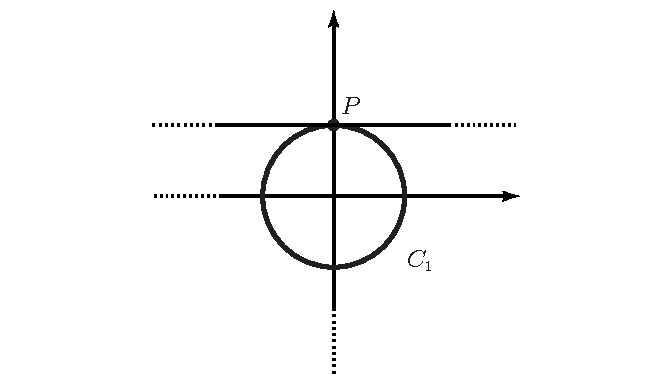
\includegraphics[trim=0cm 0cm 0cm 0cm,clip,scale=0.50]{images/planecurve1.pdf}
\end{minipage}
\end{example}
\begin{example}	Sia $C$ in $\aff{\realset^2}$ la curva di equazione $f\ \colon y^2=x^2+x^3=x^2(x+1)$, una \textbf{cubica} in quanto ha grado 3.\\
Vogliamo calcolare quali sono le rette tangenti nel punto $P=(-1,\ 0)\in C$. Consideriamo pertanto il fascio di rette passanti per $P$ e le intersechiamo con la cubica per determinare quali sono tangente con la definizione; guardiamo dunque quali hanno molteplicità di intersezione maggiore di 1.\\
Il fascio di rette per $P$ è:
\begin{equation*}
	r\colon \begin{cases}
		x=-1+tv_1\\
		y=tv_2
	\end{cases}
\end{equation*}
Con $(v_1,\ v_2)$ direzione di $r$. Sostituiamo la parametrizzazione di $r$ nell'equazione di $C$, costruendo la funzione $g\left(t\right)$:
	\begin{gather*}
		t^2v^2=(tv_1-1)^2 tv_1\\
		g(t)=(tv_1-1)^2tv_1-t^2v_2^2=t[v_1(t^2v_1^2+1-2tv_1)-tv_2^2]=t[v_1^3t^2-t(2v_1^2+v_2^2)+v_1]
	\end{gather*}
	Analizziamo cosa abbiamo trovato:
		\begin{itemize}
			\item $t=0$ è sempre una soluzione: per costruzione abbiamo preso la retta che passava per $P$, dunque $P$ è banalmente intersezione di una retta di \textit{qualsiasi} direzione con la cubica.
			\item La molteplicità di intersezione fra $C$ e $r$ in $P$ è la massima potenza di $t$ che divide $g$; pertanto è $m$ se $t^m$ è la massima potenza di $t$ che divide $g$.\\
			In questo caso, quand'è che la molteplicità di intersezione è maggiore di 1? Nell'equazione che abbiamo scritto almeno $t^2$ deve dividere $g$: l'unica possibilità per questa curva di poter raccogliere un'altro $t$ è avere $v_1=0$. Allora $r$ è la retta verticale che passa per $P$ e abbiamo determinato che esiste ed è l'\textit{unica} tangente in $P$.
		\end{itemize}
	Vediamo ora un caso in cui la retta tangente ad un punto non è unica. Consideriamo la stessa cubica ma \textit{cambiamo il punto}, prendendo l'origine $Q=(0,0)\in C$.\\
	Scriviamo il fascio di rette per $Q$:
	\begin{equation*}
		q\colon \begin{cases}
			x=tw_1\\
			y=tw_2
		\end{cases}
	\end{equation*}
	Con $(w_1,\ w_2)$ direzione. Analogamente a prima:
	\begin{gather*}
		h(t)=t^2w_1^2+t^3w_1-t^2w_2^2=t^2(w_1^2-w_2^2+tw_1^3)
	\end{gather*}
\begin{minipage}{0.75\textwidth}
Troviamo così che $t^2$ si può sempre raccogliere, dunque in questo caso la molteplicità di intersezione fra le rette e $Q$ è sempre almeno 2. In particolare, ogni retta per $Q$ ha intersezione maggiore di 2, dunque è \textit{tangente}.\\
Osserviamo che nel punto $Q$ la curva si auto-interseca: ogni retta per l'origine interseca la curva almeno due volte, quindi è tangente. Fra queste, ci sono due \textit{direzioni speciali} per cui la molteplicità è 3:
\begin{itemize}
	\item $w_1^2-w_2^2=0\implies w_1=w_2 \implies \mathcal{L}(1,1) \colon y=x$.
	\item $w_1=-w_2 \implies \mathcal{L}(1,-1) \colon y=-x$.
\end{itemize}
\end{minipage}
\hspace{-12mm}
\begin{minipage}{0.24\textwidth}
	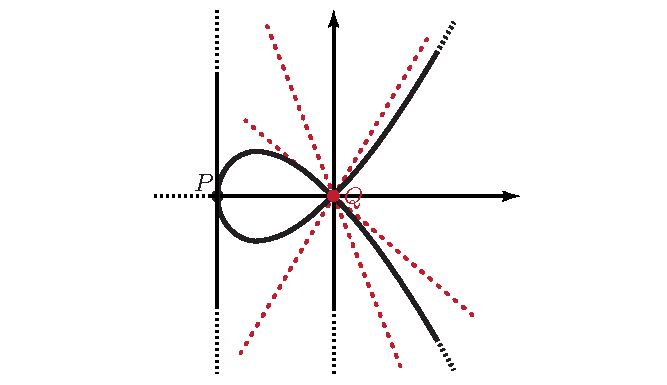
\includegraphics[trim=0cm 0cm 0cm 0cm,clip,scale=0.50]{images/planecurve2.pdf}
\end{minipage}
\end{example}
\subsubsection{Caso affine}
Sia $C\colon f(x,\ y)=0$ in $\kamp^2$ e $P=(x_0,\ y_0)$. Osserviamo che possiamo sempre scrivere il polinomio come un polinomio centrato in $x_0,\ y_0$, cioè come polinomio in $x-x_0$ e $y-y_0$ invece che come polinomio in $x$ e $y$.
\begin{gather*}
		f=\sum_{i,j\geq 0} a_{ij}x^iy^j = \sum_{i,j\geq 0} a_{ij}(x-x_0+x_0)^i(y-y_0+y_0)^j \stackrel{!}{=} 	\sum_{i,j\geq 0}b_{ij}(x-x_0)^i(y-y_0)^j\\
		\implies f(x_0,\ y_0)=b_{00}=f(P) \implies f=f(P) +\alpha (x-x_0)+\beta (y-y_0)+ \text{ termini di grado} >1
\end{gather*}
Nel passaggio indicato con (!) si stanno sottintendendo conti con il binomio di Newton.\\
\begin{define}\textsc{Derivate parziali}.\\
	Dato un polinomio $f=\sum_{i,j}a_{ij}x^iy^j\in\kamp[x,\ y]$, le \textbf{derivate parziali}\index{derivata!parziale} di $f$ sono i seguenti polinomi:
	\begin{equation}
		\frac{\partial{f}}{\partial{x}}\coloneqq \sum_{i,j}a_{ij}ix^{i-1}y^j\quad \frac{\partial{f}}{\partial{y}}\coloneqq \sum_{i,j}a_{ij}jx^iy^{j-1}
	\end{equation}
\vspace{-3mm}
\end{define}
Si verifica che $\alpha=\frac{\partial{f}}{\partial{x}}(x_0,\ y_0)$ e $\beta=\frac{\partial{f}}{\partial{y}}(x_0,\ y_0)$.
\begin{demonstration}
	Se $P\in C$, segue dai ragionamenti precedenti $f=\alpha (x-x_0)+\beta (y-y_0)+ \text{ termini di grado} >1$. Applicando la definizione di derivata parziale si hanno:
	\begin{equation*}
		\frac{\partial{f}}{\partial{x}}= \sum_{i,j}a_{ij}i\left(x-x_0\right)^{i-1}\left(y-y_0\right)^j\quad \frac{\partial{f}}{\partial{y}}= \sum_{i,j}a_{ij}j\left(x-x_0\right)^i\left(y-y_0\right)^{j-1}
	\end{equation*}
	Valutando in $P=(x_0,\ y_0)$:
	\begin{equation*}
		\frac{\partial{f}}{\partial{x}}\left(P\right)=a_{10}=\alpha\quad \frac{\partial{f}}{\partial{y}}\left(P\right)=a_{01}=\beta
	\end{equation*}
\end{demonstration}
%LEZ 35
\begin{define}\textsc{Gradiente}.\\
	Il \textbf{gradiente}\index{gradiente} $\nabla f$ è il vettore con componenti le derivate parziali:
	\begin{equation}
		\nabla f=\left( \frac{\partial{f}}{\partial{x}},\ \frac{\partial{f}}{\partial{y}} \right)
	\end{equation}
\vspace{-6mm}
\end{define}
Il gradiente valutato in $P=(x_0,\ y_0)$ è $\nabla f(P)=(\alpha,\beta)\in\kamp^2$.\\
%Adesso vogliamo intersecare con l retta genereica per P
\paragraph{Tangente e derivate parziali}
Sia $r$ la retta per $P$ con direzione $v=(v_1,v_2)$ e descrizione parametrica:
\begin{equation*}
	\begin{cases}
		x=x_0+tv_1\\
		y=y_0+tv_2
	\end{cases}
\end{equation*}
Allora:
	\begin{equation*}
		\begin{array}{ll}
			g(t)=f(x_0+tv_1,\ y+tv_2)&=\alpha tv_1+\beta tv_2 + \text{ termini in }t\text{ di grado }\geq 2 =\\
			&= (\alpha v_1+\beta v_2)t + \text{ termini in }t \text{ di grado }\geq 2
		\end{array}	
	\end{equation*}
Si hanno dunque due possibilità, che dipendono dal coefficiente di $t$:
	\begin{enumerate}
		\item	$\alpha=\beta=0$, ovvero $\nabla f =0$: il \textit{coefficiente} è nullo indipendentemente dalla retta. Allora, $\forall r$ retta per $P$,  $t^2 \mid g(t)$: la molteplicità di intersezione è $\geq 2$ e \textit{ogni} retta per $P$ è tangente a $C$ in $P$.
		\item	$\nabla f(P)=(\alpha,\beta)\neq 0$:	il coefficiente di $t$ determina in maniera \textit{univoca} la direzione della retta, che è quella \textbf{ortogonale} a $(\alpha,\beta)$. Ciò implica che $\exists !$ retta tangente a $C$ in $P$ ed è quella di direzione $(-\beta,\alpha)$ con equazione	$\alpha(x-x_0)+\beta(y-y_0)=0$, ovvero 
			\begin{equation}
				\frac{\partial{f}}{\partial{x}}(P)(x-x_0) + \frac{\partial{f}}{\partial{y}} (P)(y-y_0)=0
			\end{equation}
	\end{enumerate}
% Abbiamo così ritrovato la casistica della cubica con i punti espliciti: ogni retta è tangente oppure c'è una sola tangente alla curva nel punto.
\begin{define}\textsc{Punto singolare}.\\
	Sia $C$ una curva affine in $\kamp^2$ di equazione $f(x,\ y)=0$. Un punto $P\in C$ è detto \textit{non singolare} o \textbf{liscio}\index{punto!liscio} se $\nabla f(P)\neq 0$. Altrimenti $P$ è detto \textbf{punto singolare} \index{punto!singolare}.\\
	Una curva $C$ è detta \textbf{singolare} se ha almeno un punto singolare, altrimenti è detta curva \textit{non singolare} o \textbf{liscia}.
\end{define}
Abbiamo visto prima che se $P$ è \textit{non singolare} esiste ed è unica la tangente a $C$ in $P$. Essa ha equazione	$\frac{\partial{f}}{\partial{x}}(P)(x-x_0) + \frac{\partial{f}}{\partial{y}} (P)(y-y_0)=0$ e, essendo non singolare, almeno uno dei due coefficienti non è nullo.\\
Se invece $P$ è \textit{singolare} allora ogni retta per $P$ è tangente a $C$ in $P$.
\subsubsection{Caso proiettivo}
Vogliamo analizzare la tangenza nel \textit{caso proiettivo}. Tuttavia, prima di trattare di punti singolare o tangenti, ci servirà una proprietà dei polinomi omogenei, detta \textbf{relazione di Eulero} sui polinomi omogenei. Essa vale per un qualsiasi \textit{numero di variabili} a coefficienti in un campo \textit{qualsiasi} e mette in relazione un polinomio omogeneo con sue derivate parziali, che per costruzione sono anch'esse polinomi omogenei ma di un \textit{grado inferiore}.
\begin{theorema}\textsc{Relazione di Eulero} \index{Relazione!di Eulero} \\
	Sia $F\in\kamp[x_0,\ \ldots,\ x_n]$ polinomio omogeneo di grado $m$ e le sue derivate parziali $\frac{\partial{f}}{\partial{x_i}}\in\kamp[x_0,\ \ldots,\ x_n]$, polinomio omogenei di grado $m-1$. Si ha che:
		\begin{equation}
			\sum_{i=0}^n x_i\frac{\partial{F}}{\partial{x_i}}=mF
		\end{equation}
	\vspace{-6mm}
\end{theorema}
Nella relazione appena annunciata notiamo che moltiplichiamo ciascuna derivata parziale per $x_i$. Ciò è necessario per la \textit{buona definizione} dell'equazione: siccome le derivate parziali sono omogenee di grado $m-1$, moltiplichiamo per $x_i$ affinché la somma sia omogenea di grado $m$ come il polinomio $F$.
\begin{demonstration}
	Basta mostrarlo per un monomio $G=\lambda x_0^{j_0}\cdots x_n^{j_n}$ con $j_0+\ldots+j_n=m,\ \lambda\in\kamp$. Scrivendone le derivate parziali rispetto ad una variabile e poi moltiplicando per $x_i$ sistemiamo l'esponente $i$-esimo:
		\begin{gather*}
			\frac{\partial{G}}{\partial{x_i}}=\lambda j_i x_0^{j_0}\ldots x_i^{j_{i-1}} \ldots x_n^{j_n} \implies  x_i \frac{\partial{G}}{\partial{x_i}}=\lambda j_i x_0^{j_0}\ldots x_i^{j_i} \ldots x_n^{j_n}\\
			\implies \sum_{i=0}^n x_i\frac{\partial{G}}{\partial{x_i}} = \sum_{i=0}^n \lambda j_i x_0^{j_0} \ldots x_n^{j_n}=\lambda x_0^{j_0}\ldots x_n^{j_n} \cdot \sum_{i=0}^n j_i =mG
		\end{gather*}
\end{demonstration}
%
%il monomio è sempre lo stesso perché si moltiplica per x_i
%monomio j e somma degli esponenti è esattamente di grado, dunque =mG

%sing e non sing rette tang per piane pro
\begin{proposition}
	Sia ora $C$ in $\proj[2]{\ }$ una curva di equazione $F(x_0,x_1,x_2)=0$ con $F$ polinomio omogeneo di grado $d$. Sia $P\in C$, allora, $P$ è \textit{non singolare} $\iff$ almeno una delle derivate parziali di F non è nulla in $P$, ovvero $\exists i\in\{0,1,2\}\colon \frac{\partial{F}}{\partial{x_i}}(P)\neq 0$.\\
%allo stesso mod del caso affine con le der in p
	In tal caso esiste ed è unica la retta tangente a $C$ in $P$ ed ha equazione
		\begin{equation}
			\underbrace{frac{\partial{F}}{\partial{x_0}}(P) }_{\in\kamp}x_0 + \underbrace{frac{\partial{F}}{\partial{x_1}}(P) }_{\in\kamp}x_1 + \underbrace{frac{\partial{F}}{\partial{x_2}}(P) }_{\in\kamp}x_2 
		\end{equation}
	che ha i coefficienti dati dalle derivate parziali di $F$ in $P$.
\end{proposition}
\begin{demonstration}
	Dobbiamo verificare che per la curva affine di cui $C$ è chiusura proiettiva (ottenuta deomogeneizzando rispetto a $x_0$) si ritrovano le stesse definizioni di prima.\\
	A meno di proiettività possiamo supporre che $P=(1\colon a\colon b)\in U_0=\{x_0\neq 0\}$, ovvero che stia nella carta affine $U_0$ che è identificata a $\kamp^2$, quindi $P$ corrisponde a $(a,b)\in\kamp^2$.\\
	Poniamo $f(x,\ y)\coloneqq F(1,x,y)$ e sia $C_0$ la curva in $K^2$ di equazione $f(x,y)=0$ per cui $C$ è la chiusura proiettiva di $C_0$. Vogliamo mettere in relazione le derivate parziali di $f$ e di $F$ a partire dalla definizione stessa di $f$, 
%	che ci dice che facendo la derivate parziali di $f$ rispetto a $x$ è la sessa di 	valutata in	come polinomio, idem y, ed è una relazione fra polinomi
	per poi valutarla nel punto, ottenendo
		\begin{gather*}
			\begin{cases}
				\frac{\partial{f}}{\partial{x}} = \frac{\partial{F}}{\partial{x_1}} (1,x,y)\\
				\frac{\partial{f}}{\partial{y}} = \frac{\partial{F}}{\partial{x_2}} (1,x,y)
			\end{cases}
			\implies \textcolor{green}{\circled{\ast}}
			\begin{cases}
				\frac{\partial{f}}{\partial{x}}(a,b) = \frac{\partial{F}}{\partial{x_1}} (1,a,b)\\
				\frac{\partial{f}}{\partial{y}}(a,b) = \frac{\partial{F}}{\partial{x_2}} (1,a,b)
			\end{cases}
		\end{gather*}
	Usiamo la relazione di Eulero fra polinomi e valutiamo in $(1,a,b)$:
		\begin{gather*}
			\frac{\partial{F}}{\partial{x_0}}(1,a,b) + a\frac{\partial{F}}{\partial{x_1}}(1,a,b) + b\frac{\partial{F}}{\partial{x_2}}(1,a,b)= dF(1,a,b)=0
		\end{gather*}
	e $F(1,a,b)=0$ perché il punto sta nella curva, $P\in C$. Riusciamo così a esprimere la terza derivata parziale rispetto a $x_0$ in funzione delle altre due:
		\begin{gather*}
			\textcolor{green}{\circled{\ast\ast}}\quad \frac{\partial{F}}{\partial{x_0}}=-a\frac{\partial{F}}{\partial{x_1}} -b\frac{\partial{F}}{\partial{x_2}}
		\end{gather*}
	Quindi abbiamo che $\nabla f(a,b)=0 \iff  \nabla F(1,a,b)=(0,0,0)$, infatti se il gradiente $f$ si annulla in $P$ allora si annullano le derivate parziali rispetto a $x_1,x_2$ di $F$, allora per la relazione di Eulero anche la terza derivata parziale si annulla. Viceversa, se il gradiente di $F$ si annulla bastano le relazioni $\textcolor{green}{\circled{\ast}}$ per avere che anche il gradiente di $f$ si annulla.\\
	Il punto $P$ è \textit{non singolare} se e solo se $\nabla F(1,a,b)\neq \mathbf{0}$, dunque si ha la tesi.\\
	Vogliamo anche che la retta tangente diventi proprio quell'equazione. Supponendo $P$ non singolare, allora la retta tangente affine a $C_0$ in $P$ ha equazione $\frac{\partial{f}}{\partial{x}}(a,b)(x-a) + \frac{\partial{f}}{\partial{y}}(a,b)(y-b)=0$. La chiusura proiettiva di tale retta affine dà la retta tangente proiettiva a $C$ in $P$ ed ha equazione $\frac{\partial{f}}{\partial{x}}(a,b)(x_1-ax_0) + \frac{\partial{f}}{\partial{y}}(a,b)(x_2-bx_0)=0 $, in quanto si è omogeneizzato rispetto a $x_0$. Per $\textcolor{green}{\circled{\ast}}$ si ha che
		\begin{gather*}
			\frac{\partial{F}}{\partial{x_1}}(1,a,b)(x_1-ax_0) + \frac{\partial{F}}{\partial{x_2}}(1,a,b)(x_2-bx_0)=0 \\
			\implies  \underbrace{ \left( -a\frac{\partial{F}}{\partial{x_1}}(1,a,b) -b \frac{\partial{F}}{\partial{x_2}}(1,a,b) \right)}_{\textcolor{green}{\circled{\ast\ast}}}  x_0 + \frac{\partial{F}}{\partial{x_1}}(1,a,b) x_1 + \frac{\partial{F}}{\partial{x_2}}(1,a,b) x_2=0 \\
			\implies \frac{\partial{F}}{\partial{x_0}}(P) x_0 + \frac{\partial{F}}{\partial{x_1}}(P) x_1 + \frac{\partial{F}}{\partial{x_2}}(P) x_2
		\end{gather*}
\end{demonstration}

\begin{observe} \textsc{Rette tangenti: sistema Affine vs. Proiettivo}
	Se $C$ è una curva affine di equazione $f(x,y)=0$ per trovare i punti singolare di $C$ bisogna risolvere un sistema con l'equazione della curva e le derivate parziali di $f$. L'equazione della curva è necessaria perché potrei avere punti in cui il gradiente si annulla ma non appartengono alla curva!\\ 
	Invece se $C$ è proiettiva di equazione $F(x_0,x_1,x_2)=0$, per trovare i punti singolari di $C$ bisogna solo risolvere il sistema delle derivate parziali nulle e non serve mettere anche l'equazione della curva per via della relazione di Eulero. Infatti se $P$ annulla $\nabla F$, allora dalla relazione di Eulero si ha che:
		\begin{equation*}
			F(P)=\frac{1}{d}\left( a\frac{\partial{F}}{\partial{x_0}}(P) + b\frac{\partial{F}}{\partial{x_1}}(P) + c\frac{\partial{F}}{\partial{x_2}}(P) \right) = 0 \implies P\in C
		\end{equation*}
	Riassumendo, ecco i sistemi a confronto:
		\begin{center}
			\begin{tabular}{c|c}
				Affine & Proiettivo \\
				\hline
				$\displaystyle \begin{cases} 
					f(x,y)=0 \\		\frac{\partial{f}}{\partial{x}}(x,y)=0\\	\frac{\partial{f}}{\partial{y}}(x,y)=0
				\end{cases}$ & $\displaystyle \begin{cases}
					\frac{\partial{F}}{\partial{x_0}}=0\\	\frac{\partial{F}}{\partial{x_1}}=0\\	\frac{\partial{F}}{\partial{x_2}}=0 
				\end{cases}$
			\end{tabular}
		\end{center}
\end{observe}

\begin{examples} \label{esempi lez 35}
	\begin{enumerate}
		\item	Sia $C_0\colon x^2+x^3-y^2=0$ una curva affine. Sia $C$ la chiusura proiettiva di $C_0$ con equazione $F=x_0x_1^2+x_1^3-x_0x_2^2$, cerchiamo i punti singolari:
			\begin{gather*}
				\nabla F=0 \iff \begin{cases}
					\frac{\partial{F}}{\partial{x_0}}=x_1^2 - x_1^2=0\\
					\frac{\partial{F}}{\partial{x_1}}=2x_0x_1+3x_1^2=0\\
					\frac{\partial{F}}{\partial{x_2}}-2x_0x_2=0
				\end{cases} \implies \begin{cases}
					x_0=0 \\ x_1=0 \\ x_2=0
				\end{cases} \text{ oppure } \begin{cases}
					x_0=t \\ x_1=0 \\ x_2=0
				\end{cases}
			\end{gather*}
		di cui il primo è un assurdo, dunque $P=(1\colon 0\colon 0)$ è l'unico punto singolare di $C$ e osserviamo che corrisponde a $(0,0)\in\kamp^2$.\\
		Avevamo studiato anche il punto $Q=(-1,0)\in C_0$, vediamolo anche nel caso proiettivo in cui $Q=(1\colon -1\colon 0)\in C$ non singolare. Scriviamo la tangente $T_Q C$ grazie alle derivate parziali:	$\frac{\partial{F}}{\partial{x_0}}(Q)=1,\ \frac{\partial{F}}{\partial{x_1}}(Q)=(2x_0x_1+3x_1^2)(Q)=1,\ \frac{\partial{F}}{\partial{x_2}}(Q)=(-2x_0x_1)(Q)=0$, per cui $T_Q C\colon x_0+x_1=0$. Per ottenere la retta affine di cui è chiusura proiettiva basta porre $x_0=1$, per cui $x+1=0$, ed è coerente con l'analisi nel caso affine.\\
		Avevamo visto che nel punto singolare $P=(1\colon 0\colon 0)$, tutte le rette per $P$ hanno molteplicità di intersezione $2$ con la curva $C$ in $P$ tranne due rette speciali, quelle di direzione $(1\pm 1)$ in cui la molteplicità di intersezione è 3, pertanto $P$ è detto \textbf{nodo}. \index{nodo}
		\item	consideriamo la curva affine $C_0$ data da $f(x,y)=y-x$ e la chiusura proiettiva $C$ di equazione $F(x_0,\ x_1,\ x_2)=x_0x_2^2-x_1^3$. Siccome $\frac{\partial{F}}{\partial{x_0}} =x_2^2,\ \frac{\partial{F}}{\partial{x_1}}= -3x_1^2,\ \frac{\partial{F}}{\partial{x_2}}= 2x_0x_2$ allora $P=(1\colon 0\colon 0)$ è l'unico punto singolare di $C$, che corrisponde all'origine in $\mathcal{A}(\kamp^2)$. Consideriamo il fascio di rette per l'origine in $\mathcal{A}(\kamp^2)$ e vediamo qual è la molteplicità di intersezione per confrontarlo con il caso precedente. Sia la generica retta per l'origine $r\colon \begin{cases}
			x=tv_1 \\
			y=tv_2
		\end{cases}$ con $v=(v_1,v_2)$ direzione di $r$. La intersechiamo con $C_0$
			\begin{gather*}
				g(t)=t^2v_2^2 -t^3v_1^3=0 \implies t^2(v_2^2 -tv_1^3)=0
			\end{gather*}
		da cui segue la molteplicità di intersezione in $P$ è 2 se $v_2\neq 0$ ed è 3 se $v_2=0$.\\
		Si nota che è simile al caso precedente ma la differenza sta nel fatto che quasi tutte le rette hanno molteplicità 2 e c'è solo un'unica retta con molteplicità 3 e non 2 come nel caso precedente.\\
		Disegnandola si nota la presenza di una cuspide e attorno al punto singolare non è liscia.
%DISEGNO
	\end{enumerate}
\end{examples}

Questi erano esempi di cubiche, vediamo cosa succede per le coniche.
\begin{observe} \textsc{Punti singolari delle coniche}\\
	Sia $C$ una conica proiettiva, allora il numero di punti singolari dipende solo dal rango, ovvero
		\begin{itemize}
			\item	$\rk C=3\implies C$ non ha punti singolari
			\item	$\rk C=2 \implies C$ ha un punti singolare
			\item	$\rk C=1 \implies C$ è una retta doppia e ogni punto di $C$ è singolare
		\end{itemize}
	Infatti sia $A$ la matrice simmetrica associata a $C$, allora l'equazione associata a $C$ e le derivate parziali sono 
		\begin{gather*}
			F=x^tAX=\sum_{i,j=0}^2 a_{ij}x_ix_j \implies \frac{\partial{F}}{\partial{x_h}} = \sum_{j=0, i=h}^2 a_{hj}x_j+ \sum_{i=0, j=h}^2  a_{ih}x_i = 2\sum_{i=0}^2 a_{ih}x_i
		\end{gather*}
	Un punto $P$ rappresentato dal vettore $v$, ovvero $P=[v]$, è singolare per $C$ se le derivate parziali si annullano, cioé se $\sum_{i=0}^2 a_{hi}v_i=0\forall h=0,1,2$. In notazione matriciale, se si pensa al prodotto righe per colonne si ha che l'indice di riga di $a$ è fissato in $h$ mentre facciamo variare l'indice di colonna $i$: sia $v=\begin{psmallmatrix} v_0 \\ v_1 \\ v_2 \end{psmallmatrix}$ il vettore e $\left( Av \right)_{\text{riga }h}$ un vettore colonna, dunque la condizione con la sommatoria ci dice che $Av=0$, ovvero $v\in\ker A$.\\
	Riassumendo, i punti singolari di $C$ sono dati dai vettori che stanno nel nucleo della matrice $A$, che dipende dal rango di $A$:
		\begin{itemize}
			\item	$\rk A=3\implies \ker A=\{0 \} \implies$ nessun punto singolare
			\item	$\rk A=2\implies \dim\ker A=1 \implies$ unico punto singolare
			\item	$\rk A=1\implies F=\lambda L^2$	retta doppia, allora ogni punto di $C$ è singolare	ed è esattamente la retta proiettiva associata al nucleo di $A$: $L=\mathbb{P}(\ker A)$
		\end{itemize}
	Confrontiamolo con la classificazione delle coniche nel caso proiettiva
	o reale e complesso.\\
	Posto $\rk C=2$, nel \textit{caso complesso} $C=L_1\cup L_2$ con $L_1\neq L_2$ distinte e il punto singolare è il punto di intersezione delle due rette, ovvero $L_1\cap L_2$.\\
	Nel \textit{caso reale} a meno di proiettività di hanno 2 casi in base alla segnatura: $(1,1)$ allora $C=L_1\cup L_2$ e $P=L_1\cap L_2$, mentre se la segnatura è $(2,0)/(0,2)$ allora la forma quadratica si fattorizza su $\complexset$ e non su $\realset$ e $C$ ha come sostegno un unico punto $P$, che è proprio il punto singolare.
\end{observe}

\begin{observe}\textsc{Cubiche proiettive nel caso complesso}
	Nel piano proiettivo complesso $\proj[2]{\complexset}$ consideriamo $C$ una cubica di equazione $F=0$ con $\deg F=3$. Se la curva $C$ è riducibile, allora il polinomio $F$ è riducibile, per definizione, ma siccome il grado è basso allora è prodotto di un polinomio di grado 1 per un altro polinomio di grado 2, quali $F=G\cdot H$ con $\deg G=1$ e $\deg H=2$ pertanto il luogo degli zeri di $F$ è unione dei luoghi degli zeri di $G$ e $H$, dunque $C$ è unione di una retta e di una conica.Ci riconduciamo così a gradi più bassi.\\
	Supponiamo invece che $C$ sia irriducibile: allora $C$ non può contenere una retta, altrimenti l'equazione della retta dividerebbe il polinomio $F$. Allora $C$ ha \textit{al più un punto singolare}. Infatti, se per assurdo ne avesse almeno 2 quali $P$ e $Q$ potremmo considerare la retta $r$ che passa per $P$ e $Q$ quale $r=\overline{PQ}$, pertanto $C\cap r\supseteq \{P,q\}$ e siccome sono due punti singolari allora la molteplicità di intersezione è almeno 2. Ma ciò non è possibile perché dallo studio delle intersezioni fra una retta e una curva sappiamo che dobbiamo contare con molteplicità fino al grado della curva: qui sono $2$ punti con molteplicità $2$, ma $C$ ha grado 3, dunque la retta dovrebbe essere contenuta nella curva, ma è una contraddizione.
\end{observe}

\begin{example}
	Sia $F=x_0^3+x_1^3+x_2^3$, esso dà una curva senza punti singolari perché le derivate parziali sono multipli delle coordinate dunque non possono mai essere tutti nulli
\end{example}

		\section{Fasci di coniche proiettive}
\begin{intuit}
	Scrivere il fascio vuol dire prendere 2 coniche e considerare le coniche la cui equazione si ottiene come combinazione lineare delle due equazioni di partenza.
\end{intuit}
Siano $C_1$ e $C_2$ due coniche distinte nel piano proiettivo $\proj[2]{\ }$ di equazioni $F_1$ e $F_2$, siccome le coniche sono distinte allora $F_1$ e $F_2$ non sono proporzionali. Il \textbf{fascio di coniche} generato da $C_1$ e da $C_2$ è dato da tutte le coniche di equazione $\lambda F_1+\mu F_2=0$ con $(\lambda\colon \mu)\in \proj[1]{\ }$. Possiamo scrivere $\mathcal{F}$ come fascio e $C_{\lambda,\ \mu}$ come conica specifica ottenuta dall'equazione.\\
Notiamo che se moltiplichiamo $\lambda$ e $\mu$ per lo stesso scalare tutta l'equazione viene moltiplicata ed otteniamo la stessa conica di prima, dunque $\lambda$ e $\mu$ vanno presi in $\proj[1]{\ }$ e non solo in $\kamp$.

\begin{examples}
	\begin{enumerate}
		\item	Siano $C_1\colon x_0x_1=0$ e $C_2\colon (x_0-x_1)x_2=0$ due coniche, entrambe coppie di rette. Allora il fascio da loro generato è $C_{\lambda,\mu}\colon \lambda x_0x_1 + \mu (x_0-x_1)x_2=\lambda x_0x_1 + \mu x_0x_2 -\mu x_1x_2=0$
		\item	Siano $C_1\colon x_0x_1=0$ e $\widetilde{C_2}\colon x_0x_2=0$. Il fascio sarà $C_{\lambda,\mu}\colon \lambda x_0x_1 +\mu x_0x_2=x_0(\lambda x_1 + \mu x_2)=0$, infatti siccome $x_0=0$ appartiene ad entrambe le coniche si può raccogliere il fattore $x_0$
	\end{enumerate}
\end{examples}

Dato un fascio di coniche ci si chiede qual è il rango delle coniche del fascio.
\begin{define}\textsc{Conica Degenere} \index{conica!degenere}
	Una conica $C$ in $\proj[2]{\ }$ si dice \textbf{degenere} quando \textit{non} ha rango massimo, ovvero se $\rk C< 3$, dunque quando la matrice non è invertibile.
\end{define}

	\subsection{Studio delle coniche degeneri di un fascio}
Dato un fascio vogliamo vedere quante e quali sono le coniche degeneri del fascio.\\
Supponiamo che $C_1$ abbia come matrice simmetrica $A_1$ e $C_2$ idem con $A_2$. Allora è chiaro che la conica del fascio generata da $C_1,C_2$ sarà associata alla combinazione lineare sulle matrici: $C_{\lambda,\mu}\rightarrow \lambda A_1+\mu A_2$, matrice $3\times 3$ i cui elementi sono o $0$ o forme lineari in $\lambda$ e $\mu$.\\
Sia $D(\lambda,\mu)\coloneqq \det (\lambda A_1+\mu A_2)$, che è un polinomio omogeneo in $\lambda$ e $\mu$ che sarà nullo o di grado $3$. Si hanno due possibilità:
	\begin{itemize}
		\item	$D(\lambda,\ \mu)\equiv 0\implies$ \textit{tutte} le coniche del fascio sono degeneri
		\item	$D(\lambda,\ \mu)$ è omogeneo di grado 3, dunque le	coniche degeneri corrispondono agli zeri del polinomio $D$ su $\proj[1]{\ }$ che sono al più 3, pertanto ci sono \textit{al più 3 coniche degeneri}
	\end{itemize}
\begin{tips}
	Deduciamo dunque che o tutte le coniche del fascio sono degeneri o sono al massimo 3, quindi se in un fascio ne trovo 4 degeneri allora tutte lo sono!
\end{tips}
Nel caso complesso gli zeri sono pari al grado contato con molteplicità, dunque si ha sempre almeno una conica degenere. Ciò vale anche nel caso reale essendo il grado dispari.
		

Riscriviamo gli esempi precedenti
\begin{examples}
	\begin{enumerate}
		\item	Il fascio è $\mathcal{F}_1\colon 2(\lambda x_0x_1 +\mu x_0x_2 -\mu x_1x_2)=0$ ed ha matrice $A_{\lambda,\mu}=\begin{pmatrix}
			0 & \lambda & \mu \\
			\lambda & 0 & -\mu \\
			\mu & \mu & 0
		\end{pmatrix}$. Pertanto $D(\lambda,\mu)=\det A_{\lambda,\mu}=-\lambda(\mu^2)+\mu(-\lambda \mu)=-2\lambda\mu^2$. Ci sono solo 2 eri perché uno è doppio, e $D$ si annulla per $(\lambda\colon\mu)=(1\colon 0)$ oppure $(0\colon 1)$. Questi valori dei parametri ci restituiscono i polinomi di partenza, corrispondono dunque a $C_1$ e $C_2$, che sapevamo già essere degeneri. Abbiamo dunque scoperto che $C_1$ e $C_2$ sono le uniche coniche degeneri del fascio.
		\item	Il fascio è $\mathcal{F}_2 \colon x_0(\lambda x_1+\mu x_2)=0$. In questo caso il determinante viene identicamente nullo $D\equiv 0$ perché sono riducibili essendo coppie di rette. In questo fascio dunque tutte le coniche hanno una retta in comune.
	\end{enumerate}
\end{examples}

\begin{define} \textsc{Punti Base di un fascio di coniche} \index{punti!base}\\
	I \textbf{punti base} di un fascio di coniche sono i punti che appartengono a tutte le coniche del fascio, ovvero 
		\begin{equation*}
			\inter_{C\in\mathcal{F}} C \subset \proj[2]{\ }
		\end{equation*}
\end{define}

\begin{observe} \textsc{Punti base}\\
	I punti base di un fascio sono dati dall'interseoine delle due coniche che generano il fascio: $C_1\cap C_2$.\\
	Infatti $\displaystyle C_1\cap C_2 \supseteq \inter_{C\in\mathcal{F}} C$. Viceversa se $P\in C_1\cap C_2$ allora $F_1(P)=0$ e $F_2(P)=0 \implies (\lambda F_1 +\mu F_2)(P)=0,\forall\lambda,\mu \implies P\in C_{\lambda,\mu},\forall (\lambda\colon\mu)\in\proj[1]{\ }$, ovvero comunque si faccia la combinazione lineare viene sempre nulla.
\end{observe}

Vediamo i punti base degli esempi precedenti.
\begin{examples}
	\begin{enumerate}
		\item	Per ottenere i punti base del fascio si intersecano le coniche che lo generano:
			\begin{gather*}
				\begin{cases}
					x_0x_1=0\\
					(x_0-x_1)x_2=0
				\end{cases} \implies \begin{cases}
					x_0=x_1=0\\
					x_0=x_2=0\\
					x_1=x_2=0
				\end{cases}
			\end{gather*}
		Intersecando due rette non coincidenti si possono ottenere al più 4 punti 1+1+1+1, ma se ne ottengono meno se qualcuno di questi punti va a coincidere.\\
		In questo caso infatti si hanno 3 punti base quali $(1\colon 0\colon 0),(0\colon 1\colon 0), (0\colon 0\colon 1)$
		\item	I punti base sono dati dal sistema $\begin{cases} x_0x_1=0\\ x_0x_2=0 \end{cases}$. Si ha una retta di punti base perché $x_0=0$ è una retta comune a tutte le coniche del fascio, e $P=(1\colon 0\colon 0)$ è un altro punto base. Inoltre è il punto base del fascio di rette $\lambda x_1+\mu x_2=0$, che varia fra tutte le rette che contengono $P$.
	\end{enumerate}
\end{examples}

\begin{digression} \textsc{Nodi e Cuspidi}\\
	Un \textbf{nodo} è un punto $P$ per cui la retta "generale" per $P$ ha intersezione $2$ con la curva e ce ne sono \textit{esattamente} $2$ che hanno intersezione $>2$.\\
	Una \textbf{cuspide} è un punto in cui la retta "generale" per $P$ ha intersezione $2$ con la curva e ce n'è \textit{una sola} che ha intersezione $>2$
\end{digression}





%LEZ 36
	\subsection{Parametrizzazione delle coniche nel piano proiettivo}
Data l'equazione di una conica $F=a_{00}x_0^2+2a_{01}x_0x_1+\dots+a_{22}x_2^2$ possiamo associare a $C$ il punto $(a_{00}\colon a_{01}\colon a_{02}\colon a_{11}\colon a_{12}\colon a_{22})\in\proj[5]{\ }$, in quanto ci sono 6 coordinate. Tale punto determina univocamente la conica: entrambi sono non nulli e determinati a meno di multipli.\\
In questo modo otteniamo una corrispondenza biunivoca fra le coniche in $\proj[2]{\ }$ e $\proj[5]{\ }$, ovvero
	% https://q.uiver.app/?q=WzAsMixbMCwwLCJcXHtcXHRleHR7Y29uaWNoZSBpbiB9XFxwcm9qWzJde1xcIH0gXFx9Il0sWzIsMCwiXFxwcm9qWzVde1xcIH0iXSxbMCwxLCIxXFxjb2xvbiAxIiwwLHsic3R5bGUiOnsidGFpbCI6eyJuYW1lIjoiYXJyb3doZWFkIn19fV1d
	\[\begin{tikzcd}
		{\{\text{coniche in }\proj[2]{\ } \}} && {\proj[5]{\ }}
		\arrow["{1\colon 1}", from=1-1, to=1-3, tail reversed]
	\end{tikzcd}\]
In questo contesto Cosa vuol dire considerare un fascio di coniche?\\
Date $C_1$ e $C_2$ coniche, consideriamo il fascio $\mathcal{F}$ da loro generato. Se $C_1\colon F=\sum_{i,j}a_{ij}x_ix_j$ allora corrisponde ad un punto $A=(a_{00}\colon \cdots \colon a_{22})\in\proj[5]{\ }$. Idem per $C_2\colon G=\sum_{i,j}b_{ij}x_ix_j$ che corrisponde ad un punti $B=(b_{00}\colon\cdots\colon b_{22})\in\proj[5]{\ }$. La conica $C_{\lambda,\ \mu}$ del fascio è la combinazione lineare di $F$ e $G$, dunque i coefficienti sono la combinazione lineare dei coefficienti delle equazioni di $C_1$ e $C_2$, ovvero
	\begin{gather*}
		c_{\lambda,\mu}\colon \lambda F+\mu G=\sum_{i,j}(\lambda a_{ij}+\mu b_{ij})x_ix_j \longleftrightarrow P_{\lambda,\mu} =(\lambda a_{00}+\mu b_{00}\colon \cdots \colon \lambda a_{22}+\mu b_{22})\in\proj[5]{\ }
	\end{gather*}
Facendo variare $\lambda$ e $\mu$ si ha che il punto $P_{\lambda,\mu}$ descrive in $\proj[5]{\ }$ una retta generata dai punti $A$ e $B$ quale $\overline{AB}$, pertanto un \textit{fascio di coniche corrisponde esattamente ad una retta in $\proj[5]{\ }$}.Siccome una retta è individuata da due qualsiasi suoi punti, allo stesso modo il fascio è descritto da qualsiasi sue 2 coniche, pertanto la scelta coniche dà solo una parametrizzazione diversa del fascio.\\
Questo ci permette di dare più informazioni sui punti base
\begin{tips} \textsc{Calcolo punti base con 2 coniche qualsiasi}\\
	Dato un fascio $\mathcal{F}$ di coniche, i punti base del fascio sono dati dall'intersezione di due qualsiasi coniche del fascio purché siano distinte, ovvero da $C\cap\widetilde{C}$ dove $C$ e $\widetilde{C}$ sono 2 coniche distinte del fascio
\end{tips}
%così è molto più facile intersecare coppie di rette

\begin{observe}
	Sia $\mathcal{F}$ un fascio di coniche. Esiste sempre una conica $C$ degenere in $\mathcal{F}$ quindi usiamo $C$ per calcolare i punti base.\\
	Siccome è degenere, $C$ è l'unione di due rette linearmente indipendenti, ovvero $C=l_1\cup l_2$. Scegliamo una qualsiasi altra conica del fascio quale $\widetilde{C}$, duqneu i punti base del fascio sono dati da $C\cap\widetilde{C}=(l_1\cap\widetilde{C})\cup (l_2\cap \widetilde{C})$.\\
	Ne deduciamo che il numero di punti base di un fascio di coniche, se sono finiti, sono 4, infatti ciascuna delle due rette interseca $\widetilde{C}$ al più in 2 punti.
\end{observe}

\begin{corollary}
	Se due coniche $C_1$ e $C_2$ non hanno una retta in comune allora $\#(C_1\cap C_2)\leq 4$.
\end{corollary}
\begin{demonstration}
	$C_1\cap C_2$ sono i punti base del fascio generato da $C_1$ e $C_2$, dunque segue dall'osservazione precedente.
\end{demonstration}

\begin{tips} \textsc{Calcolo intersezione delle coniche}\\
	Abbiamo così anche un metodo per calcolare $C_1\cap C_2$ nel fascio $\mathcal{F}$ scriviamo $D(\lambda,\ \mu),$ troviamo una conica degenere $\widetilde{C}$ e poi intersechiamo con $C_1\cap\widetilde{C}$. Questo metodo è particolarmente utile nel caso avessimo a che fare con coniche irriducibili.
\end{tips}

Ci sono diversi tipi di rappresentazione geometrica dei fasci di coniche proiettive, vediamo quello più comune.
\begin{proposition}
	Siano $A,B,C,D$ 4 punti in posizione generale in $\proj[2]{\ }$. Allora la famiglia delle coniche passanti per i 4 punti è un fascio $\mathcal{F}$ avente come punti base esattamente i 4 punti, ovvero geometricamente stiamo fissando i 4 punti e considerando le coniche che passano per tutti e 4 i punti.\\
%famiglia fascio F: se la consider ocome punti di P5 descrivono esataente una retta: fissate due coniche le altre sono date da cl delle altre 2
%essere un fascio: in P5 è una retta: se guardo le eq tutte e sole che si ottengono come cl di due eq fissate/
	Inoltre $\mathcal{F}$ non contiene rette doppie e contiene esattamente 3 coniche degeneri che sono le coppie di rette che passano per questi 4 punti, ovvero
%DISEGNO
%\footnote{il disegno è fuorviante perché le rette si intersecano da qualche parte nel piano proiettivo}
	$\overline{AB}\cup\overline{CD}$, $\overline{AC}\cup \overline{BD}$, $\overline{AD}\cup\overline{BC}$.
%/è un fascio semplice perché il comportamento è quello che uno si aspetta/
\end{proposition}
\begin{demonstration}
	Siccome i 4 punti sono in posizione generale possiamo scegliere delle coordinate in $\proj[2]{\ }$ tali che i primi 3 sono i punti fondamentali e l'ultimo il punto unità, ovvero tali che $A=(1\colon0\colon0), B=(0\colon1\colon0), c=(0\colon0\colon1),d=(1\colon1\colon1)$.
	Partiamo dall'equazione di una conica generica e imponiamo che passi per i 4 punti e vediamo che condizioni vengono sui coefficienti:
		\begin{gather*}
			a_{00}x_0^2+2a_{01}x_0x_1+a_{11}x_1^2+2a_{02}x_0x_2+2a_{12}x_1x_2+a_{22}x_2^2=0\\
			\text{Per } A \colon a_{00}=0 \quad \text{Per } B \colon a_{11}=0 \quad \text{Per } C \colon a_{22}=0 \\
			\text{Per } D \colon 2a_{01}+2a{02}+2a_{12}=0 \implies a_{12}=-a_{01}-a_{02}\\
			\implies a_{01}x_0x_1+a_{02}x_0x_2-(a_01+a_02)x_1x_2=0
		\end{gather*}
	che sono le equazioni di tutte e sole le coniche che passano per $A,B,C,D$. Siccome $a_{01}$ e $a_{02}$ sono gli unici parametri rimasti adesso riscriviamo l'equazione evidenziandoli: $a_{01}x_1(x_0-x_2)+a_{02}x_2(x_0-x_1)=0$. Abbiamo così trovato esattamente un fascio di coniche  generato dalle due coniche entrambe degeneri:
		\begin{gather*}
			C_1\colon \underbrace{x_1}_{\overline{AC}} \underbrace{(x_0-x_2)}_{\overline{BD}}=0 \\
			C_2\colon \underbrace{x_2}_{\overline{AB}} \underbrace{(x_0-x_1)}_{\overline{CD}}=0
		\end{gather*}
	Abbiamo così dimostrato la prima affermazione.\\
	Per la seconda affermazione esaminiamo cosa sono queste coppie di rette e ritroviamo le rette per i punti base come evidenziato sopra. Per riuscirci osserviamo ad esempio che i punti per cui la coordinata $x_1=0$ sono proprio $A$ e $C$, pertanto $x_1=0$ è proprio $\overline{AC}$. In questo modo abbiamo già trovato due coniche delle coniche degeneri del fascio e questo ci dice anche che i punti base sono solo $A,B,C,D$, perché queste due rette si intersecano solo lì, infatti:
		\begin{gather*}
			C_1\cap C_2 = (\overline{AC}\cup \overline{BD}) \cap (\overline{AB}\cup\overline{CD}) = (\overline{AC}\cap\overline{AB}) \cup (\overline{AC}\cap\overline{CD}) \cup (\overline{BD}\cap \overline{AB}) \cup (\overline{BD}\cap \overline{CD}) =\\ 
			=\{A,B,C,D\}
		\end{gather*}
	Avremmo potuto evitare questo conto osservando che sono punti base perché per costruzione tutte le coniche passano per questi 4 punti, inoltre se sono finiti non possono essercene altri.
	Per calcolare le coniche degeneri utilizziamo l'equazione della conica generica del fascio e scriviamo la matrice divisa per due perché tanto è determinata a meno di multipli e ne calcoliamo il determinante:
		\begin{gather*}
			M=\begin{pmatrix}
				0 & a_{01} & a_{02} \\
				a_{01} & 0 & -a_{01}-a_{02}\\
				a_{02} & -a_{01}-a{02} & 0
			\end{pmatrix}\\
		\implies D=\det M= -a_{01}a_{02}(a_{01}+a_{02})+a_{02}a_{01}(-a_{01}-a_{02}) = -2a_{01}a_{02}(a_{01}+a_{02})
		\end{gather*}
	Osserviamo che è un polinomio omogeneo in $a_{01}$ e $a_{02}$ già fattorizzato in fattori lineari, pertanto si hanno esattamente 3 coniche degeneri: $a_{01}=0$ dà $C_2$, mentre $a_{02}=0$ dà $C_1$ e la terza si ottiene sostituendo nell'equazione del fascio $a_{02}=-a_{01}$, ottenendo $a_{01}x_0x_1-a_{01}x_0x_2=0$ dunque $x_0(x_1-x_2)=0$, a cui corrispondono $\overline{BC}$ e $\overline{AD}$.\\
	Tutte e tre le coniche degeneri hanno rango 2 e quindi non ci sono rette doppie nel fascio.
\end{demonstration}

\begin{tips} \textsc{Scrittura fascio coniche per 4 punti in posizione generale} \label{fascio coniche per 4 pt pos gen} \\
	Se dobbiamo scrivere un fascio di coniche per 4 punti procedere come nella dimostrazione può esser lungo, vediamo un metodo alternativo.\\
	Supponiamo di aver dati 4 punti in posizione generale e di voler scrivere il fascio $\mathcal{F}$ delle coniche che passano per questi 4 punti.
		\begin{itemize}
			\item	Scriviamo 2 delle coniche riducibili: $l_1$ equazione della retta $\overline{AB}$, $l_2$ retta $\overline{CD}$, $l_3$ retta $\overline{AC}$ e $l_4$ retta $\overline{BD}$ 
			\item	L'equazione del fascio è $\mathcal{F}\colon \lambda l_1 l_2 + \mu l_3 l_4 =0$
		\end{itemize}
\end{tips}

Considerando un punto del piano proiettivo sappiamo che se è un punto base allora appartiene a tutte le coniche del fascio, ci chiediamo ora per quante coniche passa se \textit{non} è un punto base del fascio.
\begin{proposition}
	Sia $\mathcal{F}$ un fascio di coniche e sia $P\in \proj[2]{\ }$. Se $P$ \textit{non} è un punto base di $\mathcal{F}$, allora esiste ed è unica la conica del fascio che contiene $P$.
\end{proposition}
\begin{demonstration}
	Supponiamo di avere 2 coniche quali $C_1, C_2$ che generano il fascio $\mathcal{F}$ con $C_i\colon f_i=0$. Pertanto il fascio avrà equazione $\mathcal{F}\colon \lambda F_1 +\mu F_2=0$. Il punto $P$ appartiene alla conica generale del fascio se e solo se l'equazione della conica è soddisfatta nel punto, ovvero 
		\begin{equation*}
			P\in C_{\lambda,\mu} \iff \lambda F_1(P) +\mu F_2(P)=0
		\end{equation*}
	Tale equazione può essere vista come un'equazione in $(\lambda \colon \mu)$.\\
	Siccome $P$ non è un punto base, allora non appartiene all'intersezione, dunque non è possibile che entrambe le equazioni si annullino in P, ovvero $P\notin C_1\cap C_2 \implies (F_1(P), F_2(P)) \neq (0,0)$. Pertanto l'equazione ha un'unica soluzione in $\proj[1]{\ }$ che sarà proprio $(-F_2(P)\colon F_1(P))$, ottenendo così un'unica conica del fascio che contiene $P$.
%sostituisco i valori di lamba e mu per trovare la soluzione /esempio in giallo
\end{demonstration}

Vedremo ora come 5 punti determinano una conica proiettiva.
\begin{proposition}
	Dati 5 punti distinti in $\proj[2]{\ }$ \textit{a 4 a 4 non allineati} \footnote{è una condizione più debole rispetto all'essere in posizione generale, perché potrebbero essercene 3 allineati ma non 4}, esiste ed è unica la conica $C$ che li contiene.
\end{proposition}
\begin{demonstration}
	Possiamo scegliere 4 di questi punti che sono in posizione generale, infatti consideriamo i primi 4 quali $A,B,C,D$: se sono in posizione generale ok, altrimenti ce ne sono 3 allineati, per esempio $A,B,C$. Siccome per i potesi i 4 pt non sono allineati allora $D\notin r$ con $r$ retta per $A,B,C$ e sempre per ipotesi $E\notin r$. Tralasciamo $C$ e consideriamo $A,B,D,E$: di nuovo, se sono in posizione generale ok, altrimenti 3 sono allineati, però abbiamo già che $D,E \notin r$, dunque abbiamo 3 punti allineati che possono essere $A,D,E$ oppure $B,D,E$. Supponiamo $A,D,E$, allora $B,C,D,E$ sono in posizione generale (scartiamo $A$).
	Troviamo quindi 4 punti fra	in posizione generale, dunque possiamo applicare la proposizione precedente, dunque sia $\mathcal{F}$ il fascio delle coniche passanti per $A,B,C,D$. Ma $E$ non è un punto base per $\mathcal{F}$ perché i punti base sono i 4 punti $A,B,C,D$, dunque esiste ed è unica la conica $C$ del fascio che passa per $E$, e dunque $C$ è l'unica conica che contiene i 5 punti
\end{demonstration}

Riassumendo, dati 5 punti esiste ed è unica la conica che passa per i 5 punti, e questa dimostrazione dà anche il metodo per trovare la conica che passa per tali 5 punti.

\begin{tips}
	Il metodo più semplice per trovare una conica $\mathcal{C}$ che passa per 5 punti dati $A,B,C,D,E$ in $\proj[2]{\ }$ è 
		\begin{itemize}
			\item	scegliere 4 punti in posizione generale quali $A,B,C,D$
			\item	scrivere 4 rette e il fascio $\mathcal{F} $ come nel tip precedente quale \ref{fascio coniche per 4 pt pos gen} per prima 
			\item	imporre il passaggio per il 5° punto $E$ in modo da trovare la conica $\mathcal{C}$
		\end{itemize}
	Altrimenti potremmo partire dalla conica generale e imporre il passaggio per 5 punti, ma è più lungo.
\end{tips}

\begin{observe}
	Il passaggio per un punto dà equazioni lineari omogenee sui coefficienti della conica e possiamo pensarlo come un iperpiano nel $\proj[5]{\ }$, è ragionevole aspettarsi che con 5 punti ho 5 iperpiani che in posizione generale si intersecano in solo punto.\\
	L'ipotesi sui punti a 4 a 4 non allineati serve a garantire che le condizioni lineari siano indipendenti, così da ottenere un punto nell'intersezione degli iperpiani.
\end{observe}

\begin{example}
	Se abbiamo 5 punti di cui 4 allineati, allora per ogni retta $s$ che passa per $P$ la conica $r\cup s$ contiene i 5 punti, quindi ce ne cono $\infty$ avendo infinite rette $s$.
\end{example}

%PAUSA

\begin{proposition}
	Siano 3 punti \textit{non allineati} quali $A,B,C\in\proj[2]{\ }$, e sia una retta $r$ che passi per $A$ ma non per $B$ e $C$, ovvero $A\in r$ e $B,C\notin r$. La famiglia delle coniche che passano per $A,B,C$ e sono tangenti a $r$ in $A$ è un fascio $\mathcal{F}$. I punti base del fascio sono solo $A,B,C$ e il fascio $\mathcal{F}$ non contiene rette doppie e contiene 2 coniche degeneri che sono esattamente $\overline{AB}\cup\overline{AC}$ e $r\cup\overline{BC}$, \footnote{le due coppie di rette soddisfano le condizioni necessarie: nella prima si intersecano in $A$ e la molteplicità di intersezione è 2, conta 1 per ciascuna retta, pertanto la retta è tangente, dal punto di vista dei punti singolari invece la retta è singolare, e ogni retta per $A$ è tangente; mentre la seconda coppia passa per $A,B,C$ e contiene $r$, dunque siccome quando è contenuta è tangente si ha molteplicità infinita.}
\end{proposition}
\begin{demonstration}
	Partiamo dalla conica generale e imponiamo le condizioni, ottenendo un fascio e osserviamo che vale quanto voluto.\\
	Sia $P\in r$ un punto diverso da $A$ e $P\notin\overline{BC} \implies A,B,C,P$ sono in posizione generale (a tre a tre non allineati). Scegliamo le coordinate proiettive tali che $A,B,C$ siano i punti coordinati mentre $P$ il punto unità: $A=(1\colon 0\colon 0),B=(0\colon 1\colon 0),C=(0\colon 0\colon 0\colon1)$. Allora la retta $r=\overline{AP}$ ha equazione $x_1-x_2=0$.\\
	Si consideri la conica generale $a_{00}x_0^2+2a_{01}x_0x_1+a_{11}x_1^2+2a_{02}x_0x_2+2a_{12}x_1x_2+a_{22}x_2^2=0$ e sappiamo già che il passaggio per i punti coordinati annulla la diagonale, ovvero il passaggio per $A$ implica $a_{00}=0$, per $B$ invece $a_{11}=0$ e per $C$ infine $a_{22}=0$, dunque $F=a_{01}x_0x_1+a_{12}x_1x_2+a_{02}x_0x_2$.\\
	Vogliamo scrivere le derivate parziali siccome vogliamo imporre che la retta $r$ sia tangente in $A$. Intersechiamo semplicemente con $r\colon x_1=x_2$ sostituendo in $F$ e ottenendo $a_{01}x_0x_+a_{12}x_1^2+a_{02}x_0x_1=0\implies x_1((a_{01}+a_{02})x_0+a_{12}x_1)=0$. Il primo $x_1=0$ corrisponde al fatto che $A\in r\cap C$, vogliamo che $r$ sia tangente alla conica in $A \iff x_1=0$ è l'unica soluzione $\iff$ il coefficiente di $x_0$ deve essere nullo, ovvero $a_{01}+a_{02}=0$, per cui $a_{02}=-a_{01}$. Sostituendo nell'equazione si ottiene:
		\begin{gather*}
			a_{01}x_0x_1 -a_{01}x_0x_2 + a_{12}x_1x_2=0 \implies a_{01}x_0(x_1-x_2) + a_{12}x_1x_2=0
		\end{gather*}
	Sono tutte e sole le coniche per $A,B,C$ e tangenti a $r$ in $A$, in questo modo abbiamo verificato che è un fascio $\mathcal{F}$. Vediamo quali sono le coniche che lo generano: $C_1\colon \underbrace{x_0}_{\overline{BC}} \underbrace{(x_1-x_2)}_{r}$ e $C_2\colon \underbrace{x_1}_{\overline{AC}} \underbrace{x_2}_{\overline{AB}}$. Intersecando $C_1$ e $C_2$ otteniamo i punti base:
		\begin{gather*}
			C_1\cap C_2 = (\overline{BC}\cup r) \cap (\overline{AC}\cup\overline{AB})=(\overline{BC}\cap\overline{AC}) \cup (\overline{BC}\cap\overline{AB}) \cup (r\cap\overline{AC}) \cup (r\cap\overline{AB}) =\{ C,B,A \}
		\end{gather*}
	Scriviamo la matrice per verificare che non si sono altri punti base:
		\begin{gather*}
			M=\begin{pmatrix}
				0 & a_{01} & -a_{01}\\
				a_{01} & 0 & a_{12}\\
				-a_{01} & a_{12} & 0
			\end{pmatrix}\\
			\implies D=\det M= -a_{01}(a_{01}a_{12}) -a_{01}(a_{01}a_{12}) = -2a_{01}^2 a_{12}
		\end{gather*}
	Siccome è un polinomio omogeneo di grado 3 si ha una radice doppia \footnote{i parametri nulli danno le coniche che generano il fascio}, dunque le uniche coniche degeneri sono solo $C_1$ e $C_2$.
\end{demonstration}

\begin{observe}
	Un fascio di questo tipo è l'esempio 1 di \ref{esempi lez 35}, %della scorsa lezione: 
	, ovvero consideriamo $C_1\colon x_0x_1=0$ e $C_2\colon (x_0-x_1)x_2=0$ e vediamo come sono posizionate le rette: la retta $x_0-x_1=0$ passa per il punto di intersezione delle prime 2 rette $x_0=0$ e $X_1=0$, quindi siamo nella situazione precedente: $A$ è il punto di intersezione, mentre $B$ e $C$ sono i punti di intersezione di $x_2=0$ con $x_0=0$ e $x_1=0$. Dunque $C_2$ diventa $r\cup \overline{BC}$, mentre $C_1$ è $\overline{AB}\cup \overline{AC}$.\\
	Abbiamo già verificato che i punti base sono solo 3 quali $A,B,C$ e che $C_1$ e $C_2$ sono le uniche coniche degeneri di $\mathcal{F}$ ed ora osserviamo che la retta $r$ è tangente a tutte le coniche del fascio.
\end{observe}
%DISEGNO


\begin{example} \textsc{Esercizio 4.3 FFP, risoluzione alternativa} \\
	Nel piao proiettivo reale $\proj[2]{\realset}$ consideriamo i punti $A=(0\colon 1 \colon 2), B=(0\colon 0\colon 1), C=(2\colon1\colon2), D=(3\colon0\colon1)$. Determinare, se esiste l'equazione di una conica passante per $A,B,C,D$ e tangente in $C$ alla retta $r$ di equazione $x_0-x_2=0$ che passa per $C$.\\
	\textit{Soluzione}\\
	Verifichiamo se i 4 punti sono in posizione generale verificando che sono a 3 a 3 non allineati tramite i determinanti
		\begin{gather*}
			\begin{vmatrix}
				0 & 0 & 2\\
				1 & 0 & 1\\
				2 & 1 & 2
			\end{vmatrix} \neq 0 \implies A,B,C \text{ non allineati} 
			\quad\begin{vmatrix}
				0 & 0 & 3\\
				1 & 0 & 0\\
				2 & 1 & 1
			\end{vmatrix} \neq 0 \implies A,B,D \text{ non allineati} \\
			\begin{vmatrix}
				0 & 2 & 3\\
				0 & 1 & 0\\
				1 & 2 & 1
			\end{vmatrix} \neq 0 \implies B,C,D \text{ non allineati} 
			\quad \begin{vmatrix}
				0 & 2 & 3\\
				1 & 1 & 0\\
				2 & 2 & 1
			\end{vmatrix} \neq 0 \implies A,C,D \text{ non allineati} \\
		\end{gather*}
	Dunque c'è un fascio $\mathcal{F}$ di coniche per $A,B,C,D$. Scriviamo l'equazione delle 4 rette con il determinante formale delle coordinate:
		\begin{gather*}
			\text{retta } \overline{AB} \colon \begin{vmatrix}
				x_0 & x_1 & x_2 \\
				0 & 1 & 2 \\
				0 & 0 & 1 
			\end{vmatrix} = x_0=0\\
			\text{retta } \overline{CD} \colon \begin{vmatrix}
				x_0 & x_1 & x_2 \\
				2 & 1 & 2 \\
				3 & 0 & 1 
			\end{vmatrix} = x_0- x_1 (-4) + x_2(-3)=x_0 +4x_1-3x_2=0\\
			\implies C_1\colon x_0(x_0+4x_1-3x_2)\\
			\text{retta } \overline{BD} \colon x_1=0\\
			\text{retta } \overline{AC} \colon \begin{vmatrix}
				x_0 & x_1 & x_2 \\
				0 & 1 & 2 \\
				2 & 1 & 2 
			\end{vmatrix} = -x_1(-4) +x_2(-2)= 4x_1 -2x_2=0 \implies 2x_1-x_2=0\\
			\implies C_2 \colon x_1(2x_1-x_2) \\
			\implies \text{fascio } \mathcal{F}\colon \lambda x_0(x_0+4x_1-3x_2) +\mu x_1(2x_1-x_2)=0
		\end{gather*}
	Queste sono tutte e sole le coniche che passano per $A,D$. Vogliamo la conica del fascio che è tangente alla retta $r\colon x_0-x_2=0$ in $C$. Intersechiamo la conica $C_{\lambda,\mu}$ con la retta $r$ sostituendo $x_2=x_0$ nell'equazione:
		\begin{gather*}
			\lambda x_0(x_0+4x_1-3x_0)+\mu x_1(2x_1-x_0)=0 \implies \lambda x_0(4x_1-2x_0)+ \mu x_1(2x_1-x_0)=0\\
			2\lambda x_0(2x_1-x_0)+ \mu x_1(2x_1-x_0)=0 \implies (2x_1-x_0)(2\lambda x_0 +\mu x_1)=0
		\end{gather*}
	Interpretiamo quanto trovato: sostituendo $x_2=x_0$ stiamo parametrizzando la retta $r$ come $(x_0\colon x_1\colon x_0)$ e ricordiamo che $C=(2\colon1\colon2)$, che corrisponde esattamente a $x_0=2x_1$, che è il primo fattore, dunque corrisponde alla soluzione $C$.\\
	La retta $r$ è tangente alla conica nel punto $C \iff$ anche l'altra soluzione corrisponde al punto $C \iff 2\lambda x_0 +\mu x_1$ e $-x_0+2x_1$ sono proporzionali $\iff \det \begin{pmatrix} 
		2\lambda & \mu \\
		-1 & 2
	\end{pmatrix} =0 \iff 4\lambda +\mu=0 \implies \mu=-4\lambda$, ad esempio per $\lambda=1$ e $\mu=-4$ si ha $2\lambda x_0+\mu x_1=2x_0-4x_1$. L'equazione della conica sarà $\mathcal{C} \colon x_0(x_0+4x_1-3x_2) -4x_1(2x_1-x_2)=0 \implies \mathcal{C}\colon x_0^2 +4x_0x_1 -3x_0x_2 -8x_1^2 +4x_1x_2=0$, dunque esiste ed è unica la conica cercata.
		\begin{gather*}
			F(A)=F(0,1,2)=-8+8=0 \quad F(B)=F(0,0,1)=0 \\
			F(C)=F(2,1,2)= 4+8-12-8+8 =0 \quad F(D)=F(3,0,1)=9-9=0
		\end{gather*}
%	Dunque è tangente alla conica nel punto $C=(\colon1\colon2)$
%le coordinate d c perché C corrisponde al punto, ovvero a x_0=2x_1, ovvero x_0-2x_1=0, dunque il primo fattore corrisponde alla soluzione C
%tutte le conche passano per C e r passa per C allora
%vogliamo che anche l'altra soluzione sia il punto C, quindi imponimìamo che lambda e mu dinao la stessa sol, ovvero che le forme lineari siano proporzionali, ovvero imponiamo che \det =0, ovvero che i coeff dell'eq sono multipli, ovvero \mu=-4\lambda
%poniamo \kambda=1 e \mu=-4
	Controlliamo se la conica fa quello che deve fare: passare per i punti per cui deve passare e che sia tangente a $C$. Scriviamo direttamente la tangente alla conica nel punto $C=(2\colon1\colon2)$ con le derivate parziali:
		\begin{gather*}
			\frac{\partial{F}}{\partial{x_0}} = 2x_0+4x_1-3x_2 \quad \frac{\partial{F}}{\partial{x_1}} = 4x_0-16 x_1 +4x_2 \quad \frac{\partial{F}}{\partial{x_2}} = -3x_0 +ax_1\\
			\frac{\partial{F}}{\partial{x_0}} (2,1,2) =4+4-6=2 \quad \frac{\partial{F}}{\partial{x_1}} (2,1,2) =8-16+6=0 \quad \frac{\partial{F}}{\partial{x_2}} (2,1,2) = -6+4=2\\
			\implies 2x_0-2x_2=0 \implies x_0-x_2=0
		\end{gather*}
	che è proprio la retta $r$.
\end{example} 
			









